\documentclass[12pt]{report}
\usepackage[utf8]{inputenc}
\usepackage[english,greek]{babel}
\usepackage{amsmath, amssymb}
\usepackage{graphicx}
\usepackage{indentfirst}
\usepackage{titling}
\usepackage{algorithm}
\usepackage{algorithmic}
\usepackage{subcaption}


% Redefine all algorithmic keywords to Greek
\renewcommand{\algorithmicrequire}{\textbf{Είσοδος:}}
\renewcommand{\algorithmicensure}{\textbf{Έξοδος:}}
\renewcommand{\algorithmicif}{\textbf{Αν}}
\renewcommand{\algorithmicthen}{\textbf{τότε}}
\renewcommand{\algorithmicelse}{\textbf{αλλιώς}}
\renewcommand{\algorithmicendif}{\textbf{τέλος αν}}
\renewcommand{\algorithmicfor}{\textbf{Για}}
\renewcommand{\algorithmicforall}{\textbf{Για κάθε}}
\renewcommand{\algorithmicdo}{\textbf{εκτέλεσε}}
\renewcommand{\algorithmicendfor}{\textbf{τέλος για}}
\renewcommand{\algorithmicwhile}{\textbf{Όσο}}
\renewcommand{\algorithmicendwhile}{\textbf{τέλος όσο}}
\renewcommand{\algorithmicrepeat}{\textbf{Επανάλαβε}}
\renewcommand{\algorithmicuntil}{\textbf{μέχρι}}
\renewcommand{\algorithmicloop}{\textbf{Βρόχος}}
\renewcommand{\algorithmicendloop}{\textbf{τέλος βρόχου}}
\renewcommand{\algorithmicreturn}{\textbf{Επίστρεψε}}
\renewcommand{\algorithmiccomment}[1]{\hfill\% #1}
\floatname{algorithm}{Αλγόριθμος}
\usepackage{hyperref}
\usepackage{geometry}
\geometry{margin=2.5 cm}

\pretitle{\begin{center}\LARGE\bfseries}
\posttitle{\par\large\vspace{0.5em}\subtitlepar\end{center}}

\newcommand{\subtitlepar}{}

\newcommand{\subtitle}[1]{\renewcommand{\subtitlepar}{#1}}

\title{Ομαδική εργασία για το μάθημα Θεωρία Παιγνίων}
\subtitle{Τμήμα Ηλεκτρολόγων Μηχανικών και Μηχανικών Υπολογιστών,\\ Αριστοτέλειο Πανεπιστήμιο Θεσσαλονίκης \\ Ομάδα 7}
\author{
  Γεώργιος Γκιουλέκας \\ \texttt{\foreignlanguage{english}{gkioulekg@ece.auth.gr}} \and
  Ελένη Κουμπαρίδου \\ \texttt{\foreignlanguage{english}{ekoumpar@ece.auth.gr}} \and
  Ναταλία Αναστασία Κούστα \\ \texttt{\foreignlanguage{english}{nkoustaa@ece.auth.gr}}
}
\date{Μάιος 2025}
\begin{document}

\maketitle

\chapter{Εισαγωγή}
\section{Περί της εργασίας}
Στην παρούσα αναφορά μελετάμε την αλληλεπίδραση διαφορετικών στρατηγικών του Διλήμματος του Φυλακισμένου στο πλαίσιο ενός εξελικτικού τουρνουά. Πιο συγκεκριμένα, εξετάζουμε σενάρια στα οποία οι στρατηγικές εφαρμόζονται από πληθυσμούς παικτών που συμμετέχουν σε διαδοχικές γενιές παιχνιδιών. Στο τέλος κάθε γενιάς, οι πληθυσμοί των στρατηγικών μεταβάλλονται, με βάση τις επιδόσεις τους κατά τη διάρκεια των αγώνων της περασμένης γενιάς. Η διαδικασία αυτή μοντελοποιεί τη φυσική επιλογή, όπου στρατηγικές με υψηλότερη συνολική απόδοση τείνουν να επικρατούν με την πάροδο του χρόνου.

Ο στόχος μας είναι να αναλύσουμε, τόσο θεωρητικά όσο και μέσω προσομοιώσεων, τον τρόπο με τον οποίο εξελίσσεται η κατανομή των στρατηγικών στον πληθυσμό και να διερευνήσουμε ποια στρατηγική (ή στρατηγικές) επικρατούν, υπό διαφορετικές αρχικές συνθήκες και δυναμικές εξέλιξης. Θέλουμε επίσης να διαπιστώσουμε εάν μπορούν να υπάρξουν περιοδικές ή και χαώδεις μεταβολές της πληθυσμιακής κατανομής των στρατηγικών σε βάθος γενεών, με κατάλληλη ρύθμιση των παραμέτρων του παιγνίου (πίνακας απολαβών, γύροι ανά παίγνιο) ή του μηχανισμού εξέλιξης.

\subsection{Γενική περιγραφή του παιγνίου}
Το Δίλημμα του Φυλακισμένου αποτελεί ένα χαρακτηριστικό παράδειγμα στην Θεωρία Παιγνίων και χρησιμοποιείται για την μελέτη της σύγκρουσης ατομικού και συλλογικού συμφέροντος. Πρόκειται για ένα δυαδικό πινακοπαίγνιο όπου κάθε παίκτης καλείται να επιλέξει εάν θα συνεργαστεί ($C$) ή εάν θα προδώσει ($D$) τον αντίπαλο παίκτη. Ανάλογα με τις επιλογές και των δύο παικτών, ο καθένας λαμβάνει κι από κάποια απολαβή (\foreignlanguage{english}{payoff}) που ορίζεται από τον πίνακα του παιγνίου. Οι απολαβές αυτές ικανοποιούν τις ανισότητες 
\begin{equation}
    T>R>P>S 
\end{equation}
\begin{equation}
    \label{CoopOverDef}
    2R>T+S
\end{equation}
όπου:
\begin{itemize}
    \item $T$ (\foreignlanguage{english}{Temptation}): Αμοιβή για προδοσία όταν ο αντίπαλος συνεργάζεται
    \item $R$ (\foreignlanguage{english}{Reward}): Αμοιβή για αμοιβαία συνεργασία
    \item $P$ (\foreignlanguage{english}{Punishment}): Ποινή για αμοιβαία προδοσία
    \item $S$ (\foreignlanguage{english}{Sucker's Payoff}): Τιμωρία για συνεργασία όταν ο αντίπαλος προδίδει
\end{itemize}
Ο περιορισμός \ref{CoopOverDef} προστίθεται για να ενθαρρύνει την από κοινού συνεργασία.
Στην παρούσα εργασία μελετάμε την επαναληπτική εκδοχή του παιγνίου (\foreignlanguage{english}{Iterated Prisoner's Dilemma}) όπου κάθε ζευγάρι παικτών αγωνίζεται για κάποιο αριθμό γύρων, κρατώντας ιστορικό των προηγούμενων επιλογών κάθε παίκτη, καθορίζοντας (εν δυνάμει) τις επόμενες κινήσεις τους από το εν λόγω ιστορικό. Αυτού του είδους η μνήμη επιτρέπει την ανάπτυξη σύνθετων στρατηγικών, οι οποίες με την σειρά τους εισάγουν απρόβλεπτα αποτελέσματα στην εξελικτική διαδικασία.
Θα λέμε πως δύο παίκτες 'συναντιούνται' όταν παίζουν ένα επαναληπτικό Δίλημμα του Φυλακισμένου για ορισμένο αριθμό γύρων. Θα ονομάσουμε 'συγκομιδή' το άθροισμα των απολαβών για όλους τους γύρους κατά την συνάντηση ενός παίκτη με κάποιον αντίπαλο.

Αξίζει να σημειωθεί όσον αφορά τις προσομοιώσεις πως εφόσον το σύνολο στρατηγικών που χρησιμοποιούμε δεν περιέχει στρατηγικές με τυχαιότητα, αλλά όλες καθορίζουν τις επόμενες κινήσεις βάσει του ιστορικού κινήσεων, μπορούμε να χρησιμοποιήσουμε μερική προσομοίωση. Δηλαδή σε κάθε συνάντηση δύο παικτών γνωρίζουμε ήδη από πρότερο υπολογισμό την συγκομιδή και των δύο στην συνάντησή τους, έτσι θα αποφύγουμε το μεγάλο υπολογιστικό κόστος της προσομοίωσης κάθε γύρου της συνάντησης.

\subsection{Σχετική έρευνα}
Η θεωρία παιγνίων εξελίξεων εφαρμόζεται ευρέως στην κατανόηση της συνεργασίας μεταξύ ανταγωνιστικών ατόμων, με το Δίλημμα του Φυλακισμένου να αποτελεί βασικό παράδειγμα μελετών. Η κλασική εργασία των \foreignlanguage{english}{Axelrod} και \foreignlanguage{english}{Hamilton} \cite{axelrod1981} καθιέρωσε την έννοια των επαναληπτικών τουρνουά στο Δίλημμα του Φυλακισμένου, όπου στρατηγικές όπως η \textlatin{Tit For Tat (TFT)} επικράτησαν χάρη στην απλότητα, τη συγχωρητικότητα και τη σταθερότητά τους απέναντι σε εκμεταλλευτικές τακτικές.

Στη συνέχεια, οι \foreignlanguage{english}{Axelrod} και \foreignlanguage{english}{Dion} \cite{axelrod1988} ανέλυσαν περαιτέρω τη δυναμική της συνεργασίας, ενσωματώνοντας πιο ρεαλιστικά εξελικτικά πλαίσια. Επικεντρώθηκαν στη συνθήκη υπό την οποία η συνεργασία μπορεί να εξελιχθεί και να διατηρηθεί μέσα σε πληθυσμούς που υπόκεινται σε μεταλλάξεις και επιλογή.

Η θεωρητική βάση της ανάλυσης αυτής παρέχεται από τον \foreignlanguage{english}{Alexander} \cite{alexander2023}, ο οποίος παρουσιάζει ένα πλήρες πλαίσιο της εξελικτικής θεωρίας παιγνίων. Στο έργο του, οι εξελικτικές στρατηγικές μοντελοποιούνται ως πληθυσμιακές διαδικασίες σε δυναμικά περιβάλλοντα, αξιοποιώντας Μαρκοβιανές μεταβάσεις και συναρτήσεις καταλληλότητας για την πρόβλεψη συμπεριφοράς.

Τα παραπάνω έργα παρέχουν την επιστημονική βάση για την παρούσα εργασία, η οποία υλοποιεί επαναληπτικά τουρνουά με πληθυσμιακή δυναμική (\foreignlanguage{english}{fitness dynamics} και \foreignlanguage{english}{imitation dynamics}) στο πλαίσιο του Διλήμματος του Φυλακισμένου, με σκοπό τη διερεύνηση των συνθηκών όπου διάφορες στρατηγικές μπορούν να κυριαρχήσουν ή να συνυπάρξουν με άλλες.

\section{Εγχειρίδιο Χρήσης}
Η εν λόγω εργασία παραδίδεται είτε ως \foreignlanguage{english}{MATLAB toolbox} σε ένα αρχείο \foreignlanguage{english}{.zip}, ή ως σύνδεσμος σε ένα \foreignlanguage{english}{Github Repository}.

Στην πρώτη περίπτωση ο χρήστης πρέπει αρχικά να εξάγει το αρχείο σε οποιοδήποτε προορισμό στο σύστημά του. Στην δεύτερη περίπτωση πρέπει να ανοίξει το \foreignlanguage{english}{Git Bash} στον επιθυμητό προορισμό στο σύστημά του και να γράψει την εντολή 
\begin{center}
    \foreignlanguage{english}{\textit{git clone https://github.com/geogkioul/EvolutionaryGamesToolbox.git}}
\end{center}
 Έπειτα θα χρειαστεί να ανοίξει το \foreignlanguage{english}{MATLAB} και να περιηγηθεί στον φάκελο της εργασίας \foreignlanguage{english}{EvolutionaryGamesToolbox} είτε με τον ενσωματωμένο περιηγητή του \foreignlanguage{english}{MATLAB} ή με χρήση της εντολής \foreignlanguage{english}{'cd'}. Όταν θα βρίσκεται στον κατάλληλο φάκελο θα χρειαστεί να τρέξει στο \foreignlanguage{english}{MATLAB} την εντολή
\begin{center}
\foreignlanguage{english}{\textit{addpath(genpath(pwd));}}
\end{center} προκειμένου να ρυθμίσει το \foreignlanguage{english}{path} ώστε να μπορεί να τρέξει όλες τις συναρτήσεις και τα \foreignlanguage{english}{scripts}.

Αφού το κάνει αυτό πλέον μπορεί να τρέξει οποιοδήποτε από τα πειράματα που θα αναλύσουμε παρακάτω στην παρούσα αναφορά ή ακόμη να τρέξει δικά του πειράματα με χρήση των κατάλληλων συναρτήσεων, ή με ρύθμιση των παραμέτρων στα ήδη υπάρχοντα πειράματα. Όλα τα πειράματα που παραθέτουμε στην αναφορά αυτή μπορούν να βρεθούν στον φάκελο \foreignlanguage{english}{\textit{"/Examples/"}} και είναι χωρισμένα σε επιμέρους φακέλους για \foreignlanguage{english}{Fitness} ή \foreignlanguage{english}{Imitation Dynamics}. Τα διαγράμματα που προκύπτουν από όλα τα πειράματα μπορούν επίσης να βρεθούν στον ίδιο φάκελο \foreignlanguage{english}{\textit{"/Examples/"}} χωρισμένα επίσης σε υποφακέλους ανά εξελικτική δυναμική.

Παρέχονται οδηγίες χρήσης για την κάθε συνάρτηση τόσο στην παρούσα αναφορά (\ref{documentation}) όσο και στο αρχείο \foreignlanguage{english}{\textit{"/Documentation/matlab\_toolbox\_documentation.txt"}}.


\chapter{Εξελικτικά Τουρνουά}
Σε κάθε γενιά των εξελικτικών τουρνουά έχουμε μια κατανομή των στρατηγικών στον σταθερό πληθυσμό. Αφού όλοι οι παίκτες του πληθυσμού συναντηθούν, αθροίζουμε τις συγκομιδές για όλους τους παίκτες μιας στρατηγικής ορίζοντας έτσι την \label{συνολική απόδοση}συνολική απόδοση αυτής. Ο τρόπος με τον οποίο εκμεταλλευόμαστε αυτές τις αποδόσεις των στρατηγικών για να καθορίσουμε την σύσταση του πληθυσμού της επόμενης γενιάς ορίζει τις διαφορετικές εξελικτικές δυναμικές. Ακολούθως θα εξετάσουμε δύο από αυτές τις δυναμικές.

\section{\foreignlanguage{english}{Fitness Dynamics}}
\subsection{Διαδικασία Εξέλιξης}
Στην περίπτωση που χρησιμοποιούμε \foreignlanguage{english}{Fitness Dynamics}, το ποσοστό αντιπροσώπευσης μιας στρατηγικής στον πληθυσμό της επόμενης γενιάς προκύπτει από τον λόγο της απόδοσης αυτής της στρατηγικής ως προς το άθροισμα αποδόσεων όλων των στρατηγικών στην τρέχουσα γενιά. Έστω δηλαδή μια στρατηγική Α της οποίας οι παίκτες έχουν άθροισμα συγκομιδών διπλάσιο από αυτούς μιας άλλης στρατηγικής Β στο τέλος μιας γενιάς. Τότε ο πληθυσμός της Α στην επόμενη γενιά θα είναι διπλάσιος από αυτόν της Β.

Πιο συγκεκριμένα, ξεκινούμε από μια συγκεκριμένη κατανομή των στρατηγικών στον πληθυσμό ($POP_0$) και έπειτα για κάθε γενιά βάζουμε κάθε πιθανό ζευγάρι παικτών να παίξουν ένα επαναληπτικό ΔΦ. Όταν γίνουν όλες οι $\binom{N}{2}$ πιθανές συναντήσεις υπολογίζουμε το άθροισμα των συγκομιδών για κάθε παίκτη μιας στρατηγικής. Παράλληλα, υπολογίζουμε το σύνολο συγκομιδών όλων των παικτών για την τρέχουσα γενιά, ανεξαρτήτως στρατηγικής. Για να βρούμε την τιμή \foreignlanguage{english}{Fitness} μιας στρατηγικής θεωρούμε τον λόγο της απόδοσης αυτής (άθροισμα συγκομιδών των παικτών της) ως προς την συνολική συγκομιδή (άθροισμα συγκομιδών όλων των παικτών).

Έτσι μπορούμε να καθορίσουμε την κατανομή των στρατηγικών στον πληθυσμό για την επόμενη γενιά. Πολλαπλασιάζουμε το σταθερό μέγεθος του πληθυσμού με την τιμή \foreignlanguage{english}{Fitness} κάθε στρατηγικής, ώστε να βρούμε το πλήθος παικτών που πρόκειται να την υιοθετήσουν στην επόμενη γενιά. Το κάνουμε αυτό για κάθε στρατηγική και έτσι έχουμε την νέα πληθυσμιακή κατανομή. Επαναλαμβάνουμε τα παραπάνω βήματα για προκαθορισμένο αριθμό γενεών.

\begin{algorithm}[H]
\caption{Εξέλιξη με \foreignlanguage{english}{Fitness Dynamics}}
\label{alg:FitnessDyns}
\begin{algorithmic}[1]
\REQUIRE Αριθμός παικτών $N$, πίνακας απολαβών παιγνίου $B$, αριθμός γύρων ανά συνάντηση $T$, σύνολο στρατηγικών $S$, αριθμός γενεών $J$, αρχική κατανομή πληθυσμού $POP_0$
\STATE Ανάθεση στρατηγικής σε κάθε παίκτη σύμφωνα με το $POP_0$
\FOR{κάθε γενιά $j = 1$ έως $J$}
    \FOR{κάθε ζεύγος παικτών $(i, k) \in \{1,2,\dots,N\}\times\{1,2,\dots,N\}$ με $i \ne k$}
        \STATE Οι παίκτες $i$ και $k$ παίζουν ένα επαναληπτικό ΔΦ με $T$ γύρους
        \STATE Καταγραφή της συνολικής απόδοσης κάθε παίκτη από όλα τα παιχνίδια
    \ENDFOR
    \FOR{κάθε παίκτη $n$}
        \STATE $g(n) \gets$ το άθροισμα αποδόσεων του παίκτη $n$ από όλα τα παιχνίδια της γενιάς
    \ENDFOR
    \FOR{κάθε στρατηγική $s$}
        \STATE $fit(s) \gets \dfrac{\sum_{n \in s} g(n)}{\sum_{n=1}^{N} g(n)}$ \label{fitness_percentage}
        \STATE Ο νέος πληθυσμός για τη στρατηγική $s$: $POP(s) \gets N \cdot fit(s)$ \label{float_pops}
    \ENDFOR
\ENDFOR
    \end{algorithmic}
\end{algorithm}

Η τιμή \foreignlanguage{english}{Fitness} όπως ορίζεται στην σειρά \ref{fitness_percentage} του παραπάνω ψευδοκώδικα δεν θα είναι κατ' ανάγκη ακέραιος αριθμός. Αυτό δεν μας πειράζει στην θεωρητική ανάλυση και το επιτρέπουμε (δηλαδή θα έχουμε και μη ακεραίους πληθυσμούς). Στην προσομοίωση ωστόσο, θέλουμε οι πληθυσμοί που θα βγάλουμε για κάθε στρατηγική να είναι ακέραιοι. Για να το πετύχουμε αυτό διατηρώντας παράλληλα την αναλογία \foreignlanguage{english}{fitness} στον πληθυσμό της νέας γενιάς χρησιμοποιούμε τον παρακάτω αλγόριθμο:
\begin{algorithm}[H]
\caption{Συνάρτηση \foreignlanguage{english}{POP\_Redistribute} για μετατροπή πληθυσμών σε ακεραίους}
\label{alg:PopRedist}
\begin{algorithmic}[1]
    \REQUIRE Τιμές \foreignlanguage{english}{fitness} για κάθε στρατηγική $fit(s)$, συνολικό μέγεθος πληθυσμού $N$
    \FORALL{στρατηγική $s \in S$}
    \STATE $float\_pop(s) \gets N\cdot fit(s)$
    \STATE $int\_pop(s) = \lfloor {float\_pop(s)} \rfloor$
    \STATE $residual(s) = float\_pop(s) - int\_pop(s)$
    \ENDFOR
    \STATE $remaining = N - \sum_{s \in S}{int\_pop(s)}$ \COMMENT{Παίχτες που μένει να ανατεθούν}
    \STATE Ταξινόμησε τα $residual$ κατά φθίνουσα σειρά για να βρεις ποιές στρατηγικές έχασαν περισσότερο κατά την στρογγυλοποίηση. 
    \STATE Κράτα τα \foreignlanguage{english}{indexes} των στρατηγικών με τα $\#remaining$ το πλήθος μεγαλύτερα $residual$
    \FORALL{στρατηγική $s \in indexes$}
    \STATE $int\_pop(s) \gets int\_pop(s)+1$
    \ENDFOR
    \RETURN $int\_pop$ \COMMENT Ακέραιοι πληθυσμοί που διατηρούν την αναλογία των $fitness$
\end{algorithmic}
\end{algorithm}
Είναι λογικό πως αναμένουμε ελαφρώς διαφορετικά αποτελέσματα στην θεωρητική ανάλυση και στην προσομοίωση, καθώς στην θεωρητική ανάλυση λόγω του ότι επιτρέπουμε μη ακέραιο πλήθος παικτών, μπορεί να υπάρξει σύγκλιση του πληθυσμού σε μια κατάσταση όπου υπάρχουν στρατηγικές με μη ακέραιους παίκτες. Αυτό στην προσομοίωση δεν μπορεί να συμβεί επειδή χρησιμοποιούμε την \foreignlanguage{english}{POP\_Redistribute}. Θα εξετάσουμε παρακάτω πως επηρεάζει αυτή η διαφορά την εξέλιξη των στρατηγικών.

\subsection{Πειράματα}
Τα πειράματα που διεξήχθησαν βασίζονται στην ανάλυση που πραγματοποιήθηκε στην δημοσίευση \cite{mathieu1999}. Σε κάθε πείραμα παραθέτουμε τρία γραφήματα του εξελικτικού πρωταθλήματος:

\begin{itemize}
    \item Τα αποτελέσματα της δημοσίευσης \cite{mathieu1999} που βασίζονται στην θεωρητική ανάλυση που περιγράφεται στην ίδια δημοσίευση.
    \item Το γράφημα που προκύπτει από τον κώδικα που δημιουργήσαμε για την αναπαραγωγή της θεωρητικής ανάλυσης της δημοσίευσης \cite{mathieu1999}.
    \item Το γράφημα που προκύπτει από τον Αλγόριθμο \ref{alg:FitnessDyns} για την προσομοίωση του εξελικτικού πρωταθλήματος.
\end{itemize}
Όλα τα γραφήματα μπορούν να βρεθούν στον φάκελο \foreignlanguage{english}{"examples/Figures Fitness Dynamics"}. Τα αποτελέσματα της δημοσίευσης έχουν όνομα αρχείου έναν σκέτο αριθμό (το αντίστοιχο γράφημα από την δημοσίευση), τα γραφήματα θεωρητικής ανάλυσης έχουν όνομα \foreignlanguage{english}{exampleX}, όπου $X$ το αντίστοιχο πείραμα της δημοσίευσης και τέλος τα γραφήματα των προσομοιώσεων είναι αυτά με το επίθεμα \foreignlanguage{english}{"-sim"}.
Τα αντίστοιχα \foreignlanguage{english}{Matlab Scripts} που δημιουργούν τα γραφήματα θεωρητικής ανάλυσης και προσομοίωσης μπορούν να βρεθούν στον φάκελο \foreignlanguage{english}{"examples/Scripts Fitness Dynamics"}.

\subsubsection{Εξέλιξη 'πονηρής' στρατηγικής}
Στο Σχήμα \ref{fig:fig_fit_1} παρουσιάζονται τα αποτελέσματα του εξελικτικού πρωταθλήματος για τις στρατηγικές \foreignlanguage{english}{per\_cd, per\_ddc} και \foreignlanguage{english}{soft\_majo} με αρχικό πληθυσμό 100 ατόμων για κάθε στρατηγική.

Παρατηρούμε ότι τα αποτελέσματα της θεωρητικής ανάλυσης αλλά και της προσομοίωσης διαφέρουν από το αναμενόμενο αποτέλεσμα \ref{fig:fig_fit_1_a}. Αυτό που θα περιμέναμε είναι, ότι, ενώ στα αρχικά σταδια της εξέλιξης του πρωταθλήματος η στρατηγική \foreignlanguage{english}{per\_cd} φαίνεται να επικρατεί, στη συνέχεια η στρατηγική \foreignlanguage{english}{per\_ddc} ανακάμπτει και τελικά νικάει το παιχνίδι. Ωστόσο στα αποτελέσματα των προσομοιώσεων μας η δυναμική του παιχνιδιού φαίνεται να είναι διαφορετική, αφού μετά τη 40ή γενιά αντί οι παίκτες της στρατηγικής \foreignlanguage{english}{soft\_majo} να μηδενιστούν, αυξάνονται, επεκτείνοντας έτσι την διάρκεια του παιχνιδιού.

\begin{figure}[htbp]
    \centering

    \begin{subfigure}[b]{0.5\linewidth}
        \centering
        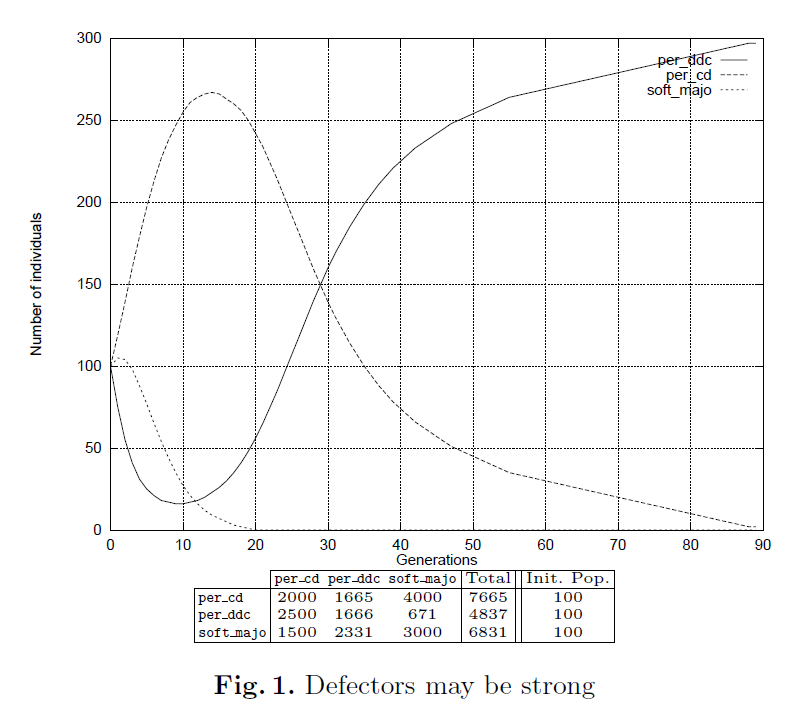
\includegraphics[width=\linewidth]{Figures Fitness Dynamics/1.png}
        \caption{Θεωρητικό αποτέλεσμα από προηγούμενη δημοσίευση. \textit{Πηγή:} \protect\cite{mathieu1999}}
        \label{fig:fig_fit_1_a}
    \end{subfigure}
    \hfill
    \begin{subfigure}[b]{0.5\linewidth}
        \centering
        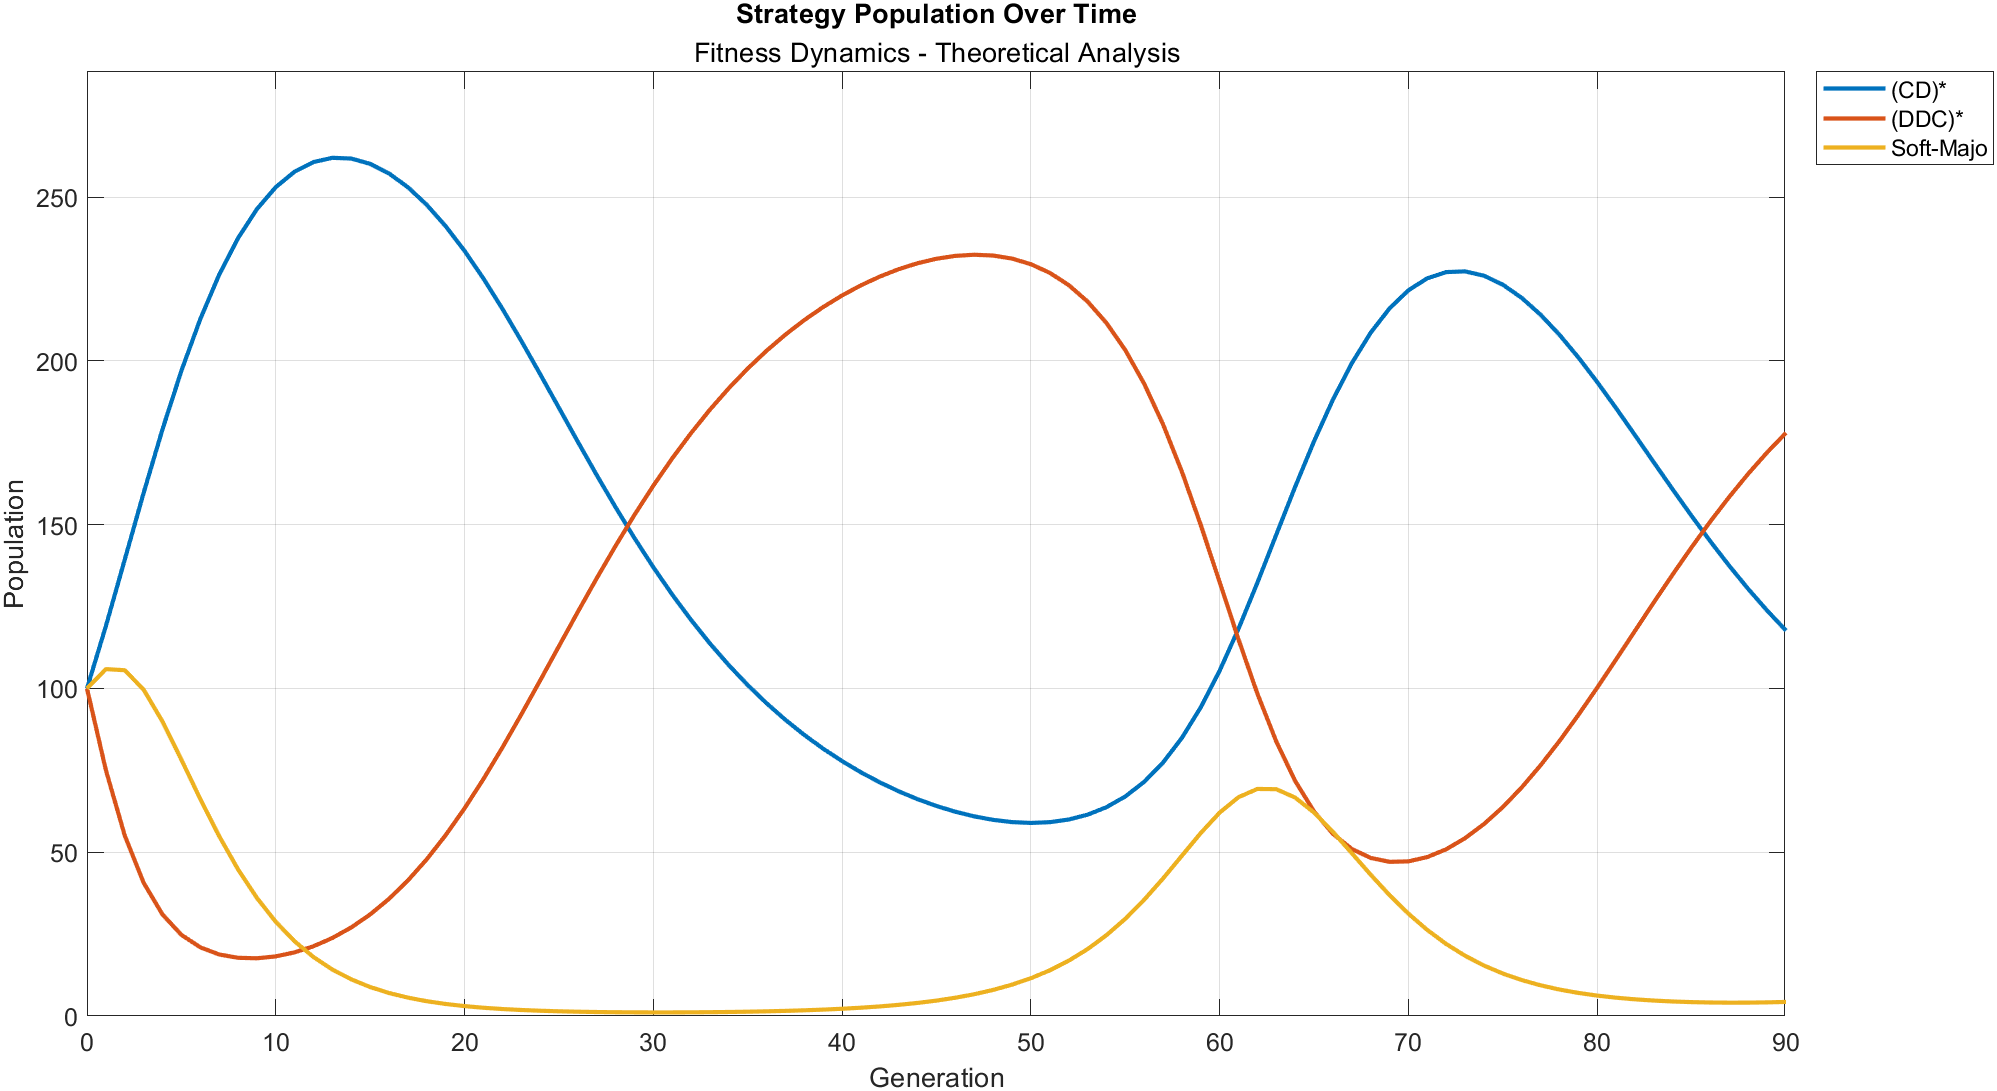
\includegraphics[width=\linewidth]{Figures Fitness Dynamics/example1.png}
        \caption{Θεωρητικό εξελικτικό πρωτάθλημα}
        \label{fig:fig_fit_1_b}
    \end{subfigure}
    \hfill
    \begin{subfigure}[b]{0.5\linewidth}
        \centering
        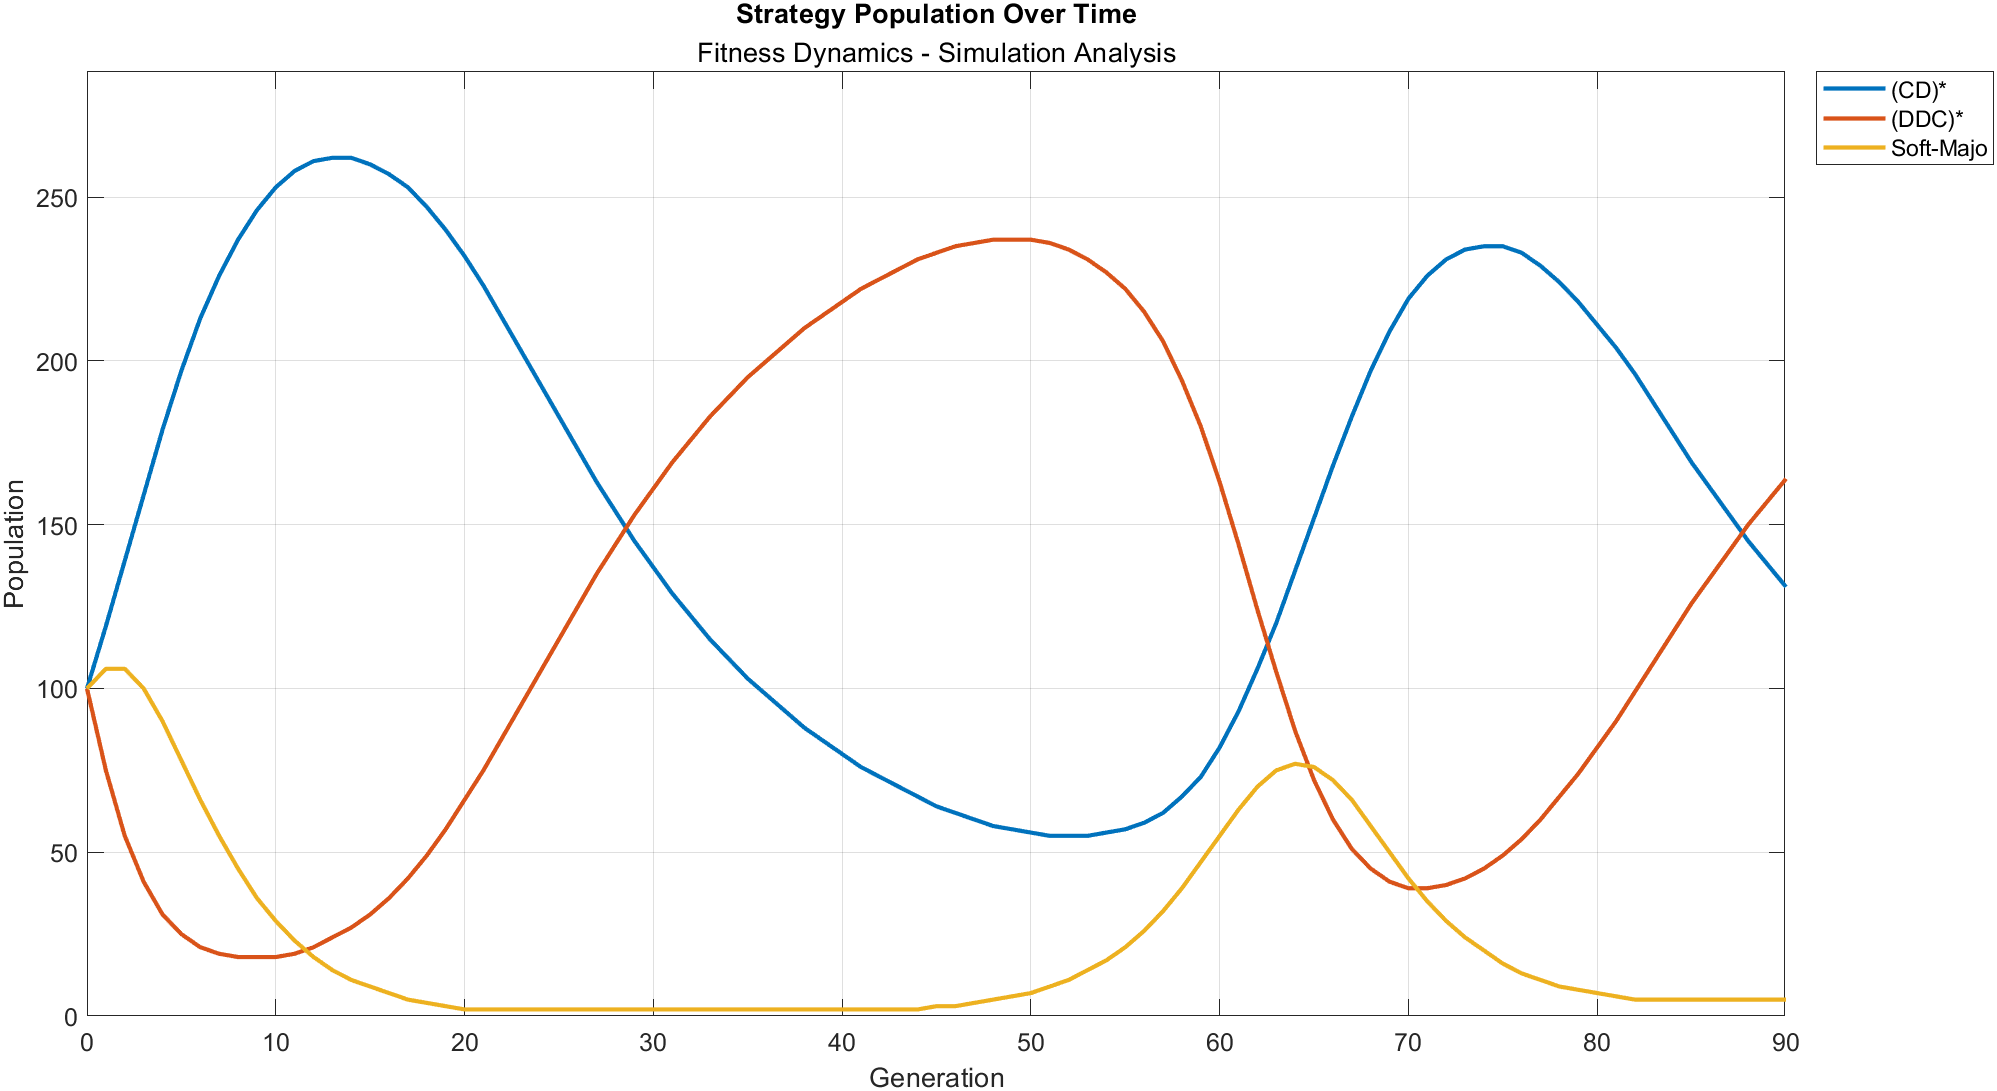
\includegraphics[width=\linewidth]{Figures Fitness Dynamics/example1-sim.png}
        \caption{Προσομοίωση εξελικτικού πρωταθλήματος}
        \label{fig:fig_fit_1_c}
    \end{subfigure}

    \caption{Αποτελέσματα πειράματος 1 - \foreignlanguage{english}{Script: example1.m}}
    \label{fig:fig_fit_1}
\end{figure}


\subsubsection{Εμφάνιση μονότονης συγκλίσης}
Στο Σχήμα \ref{fig:fig_fit_2} παρουσιάζονται τα αποτελέσματα του εξελικτικού πρωταθλήματος για τις στρατηγικές \foreignlanguage{english}{tit\_for\_tat}, \foreignlanguage{english}{gradual} και \foreignlanguage{english}{per\_cd}, με αρχικό πληθυσμό 100 ατόμων για κάθε στρατηγική. Παρατηρείται ότι όλα τα αποτελέσματα του πειράματος συγκλίνουν. Επιπλέον, διαπιστώνεται ότι η εξέλιξη των πληθυσμών είναι ομαλή και σταθερή, με ελάχιστες διακυμάνσεις, γεγονός που υποδηλώνει μονότονη σύγκλιση.

\begin{figure}[htbp]
    \centering

    \begin{subfigure}[b]{0.5\linewidth}
        \centering
        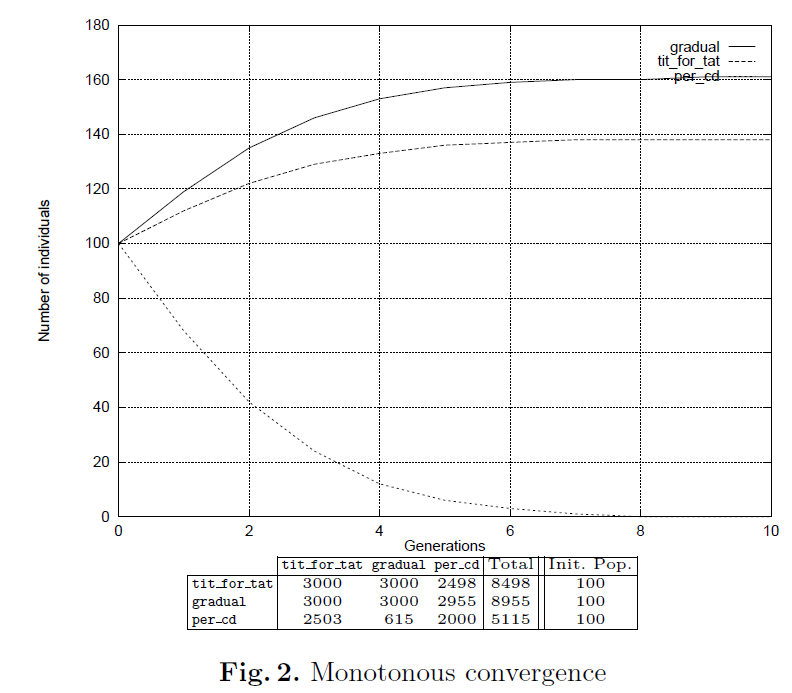
\includegraphics[width=\linewidth]{Figures Fitness Dynamics/2.png}
        \caption{Θεωρητικό αποτέλεσμα από προηγούμενη δημοσίευση. \textit{Πηγή:} \protect\cite{mathieu1999}}
        \label{fig:fig_fit_2_a}
    \end{subfigure}
    \hfill
    \begin{subfigure}[b]{0.5\linewidth}
        \centering
        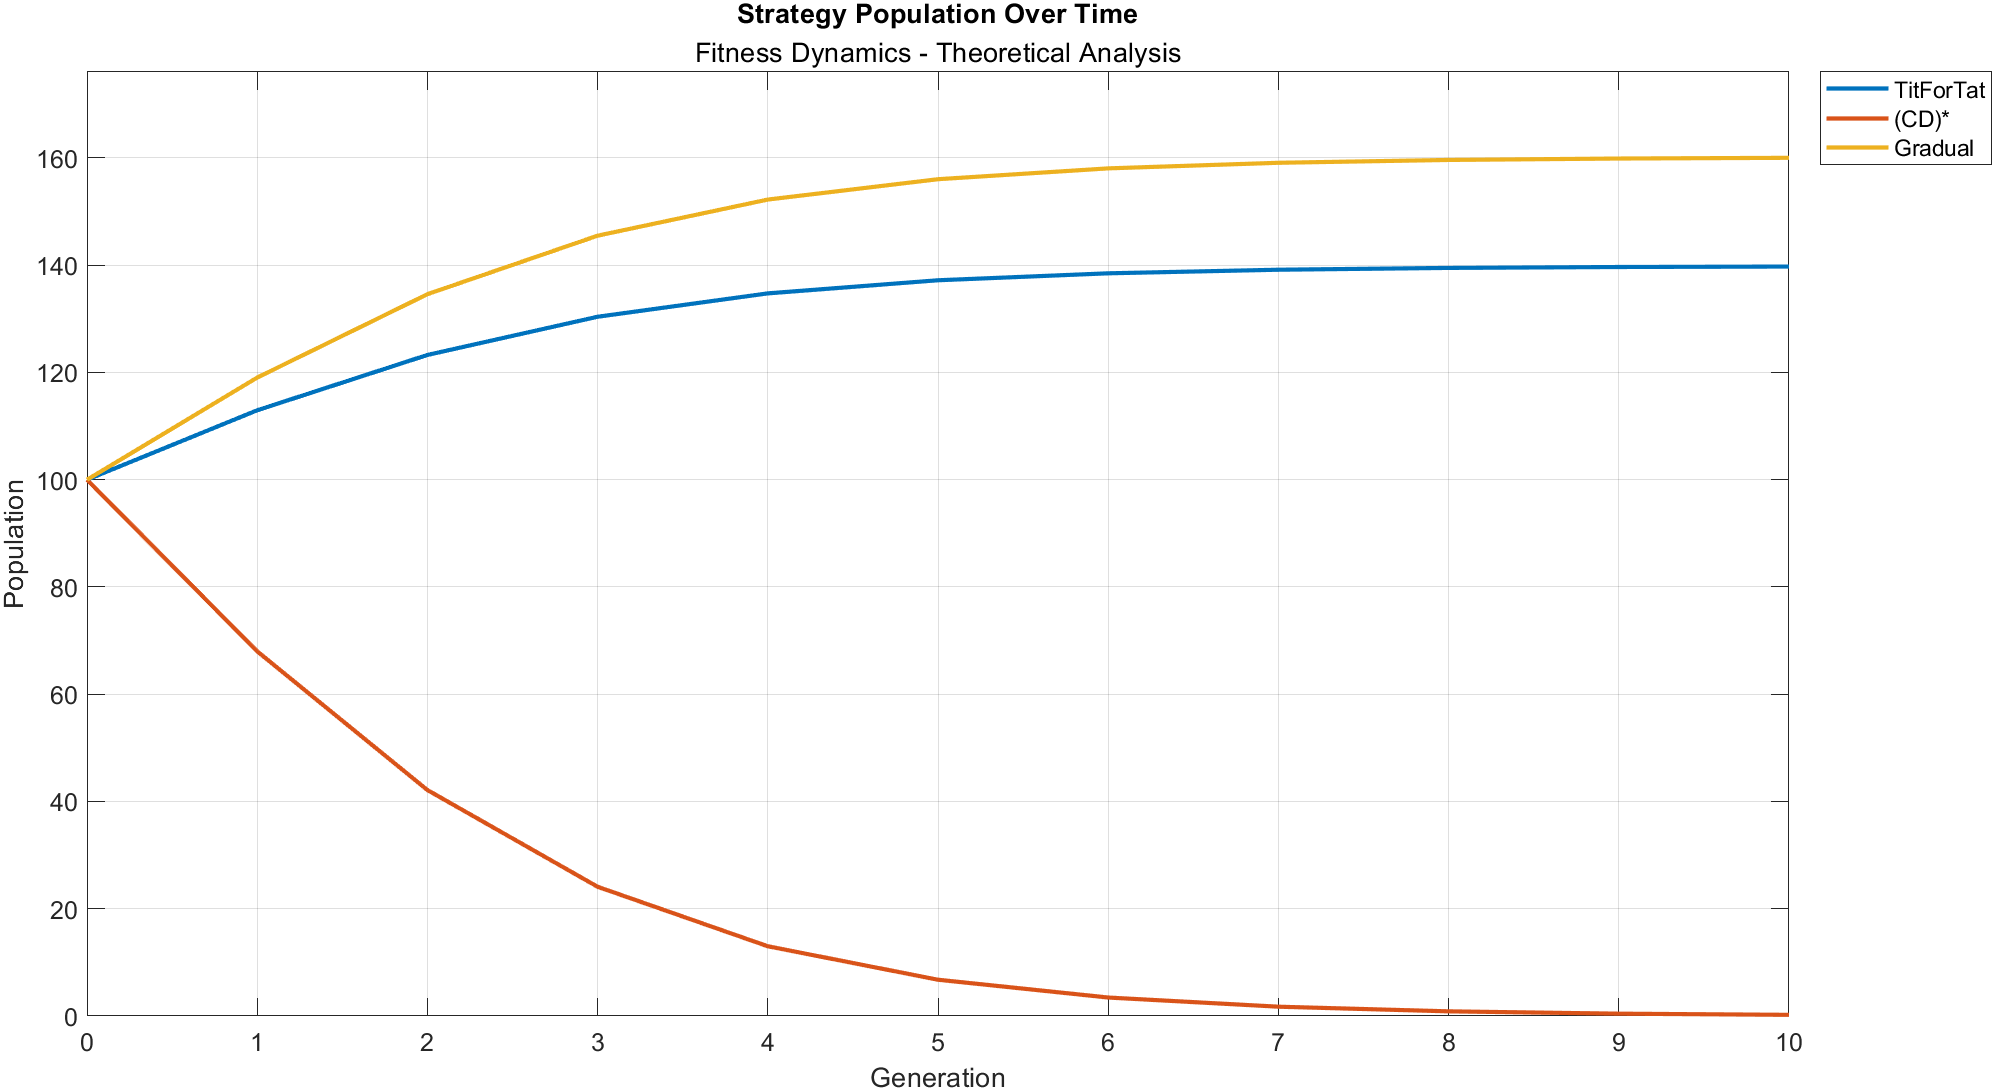
\includegraphics[width=\linewidth]{Figures Fitness Dynamics/example2.png}
        \caption{Θεωρητικό εξελικτικό πρωτάθλημα}
        \label{fig:fig_fit_2_b}
    \end{subfigure}
    \hfill
    \begin{subfigure}[b]{0.5\linewidth}
        \centering
        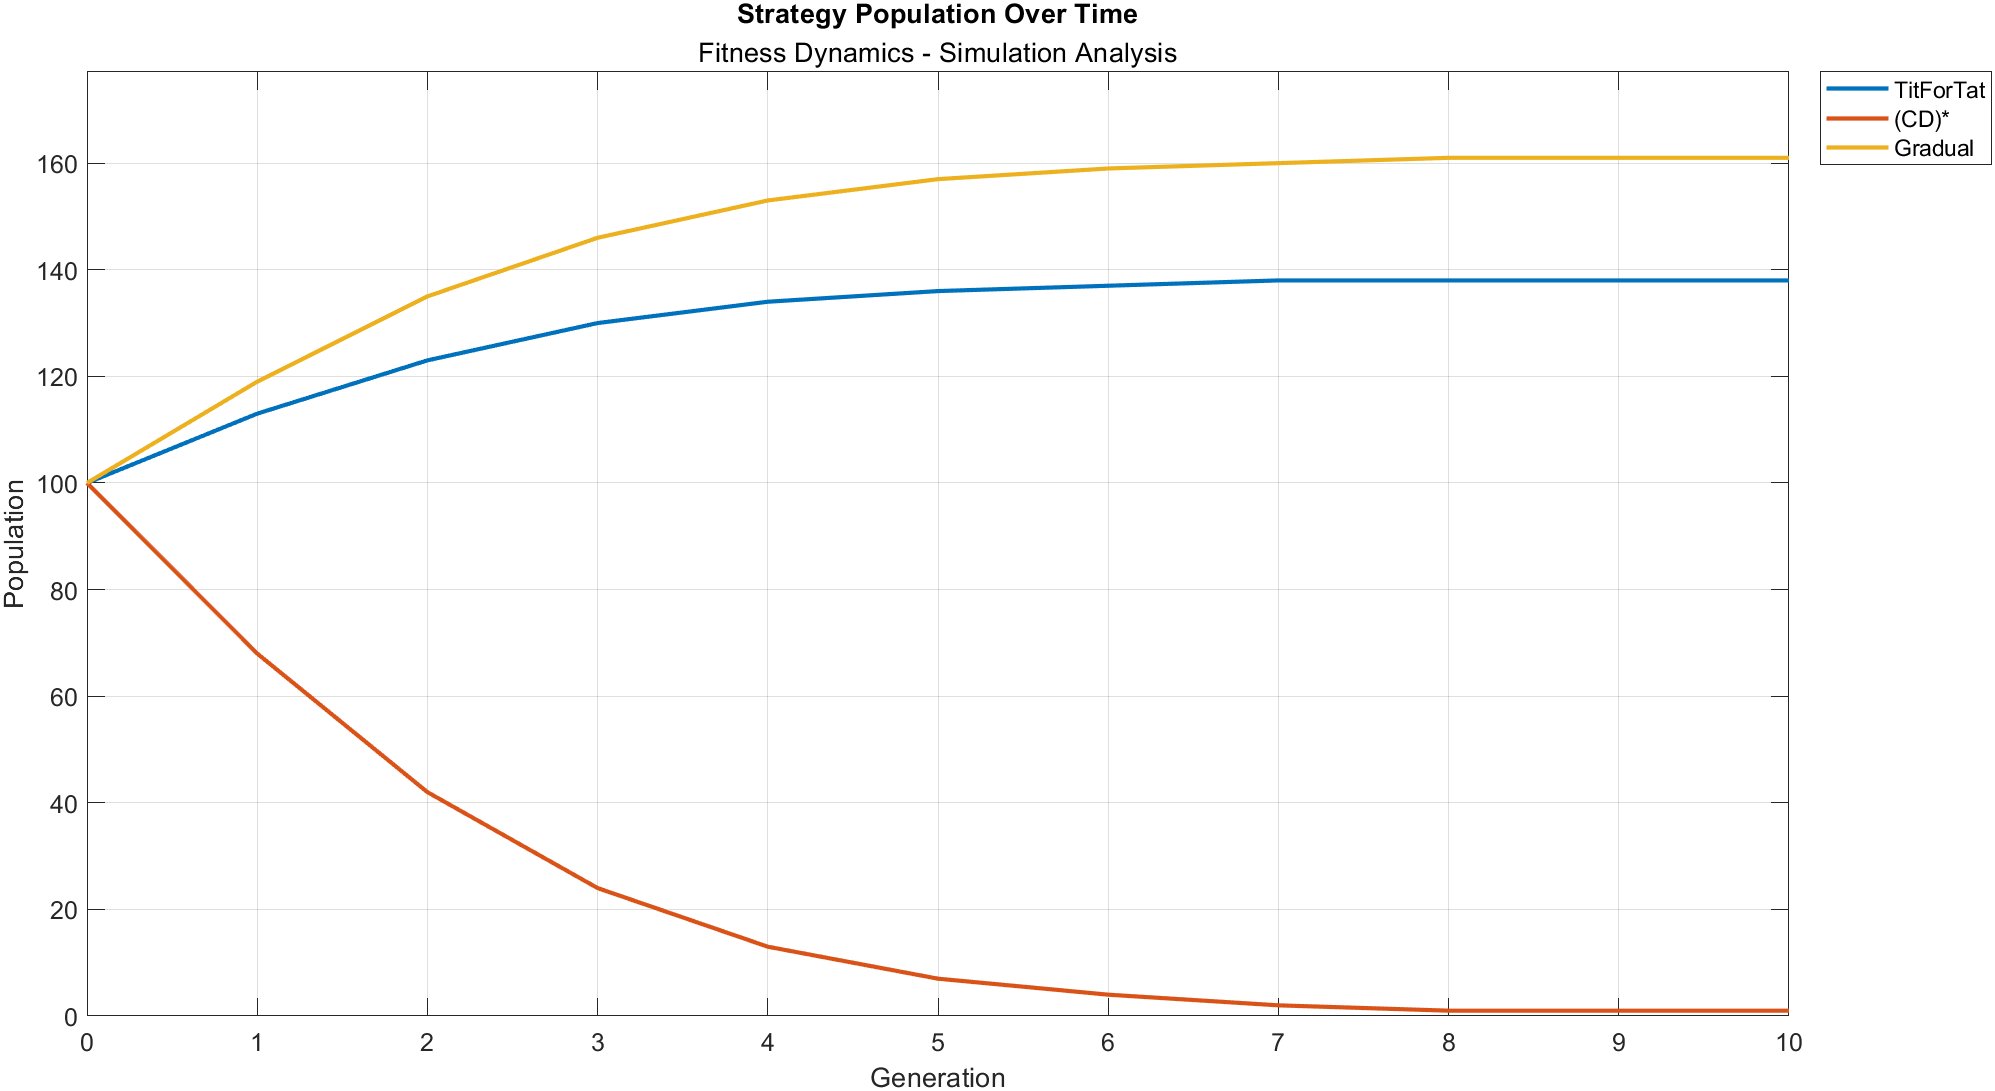
\includegraphics[width=\linewidth]{Figures Fitness Dynamics/example2-sim.png}
        \caption{Προσομοίωση εξελικτικού πρωταθλήματος}
        \label{fig:fig_fit_2_c}
    \end{subfigure}

    \caption{Αποτελέσματα πειράματος 2 - \foreignlanguage{english}{Script: example2.m}}
    \label{fig:fig_fit_2}
\end{figure}


\subsubsection{Εμφάνιση εξασθενημένων ταλάντωσεων}
Στο Σχήμα \ref{fig:fig_fit_3} παρουσιάζονται τα αποτελέσματα του εξελικτικού πρωταθλήματος για τις στρατηγικές \foreignlanguage{english}{per\_ccd, per\_ddc} και \foreignlanguage{english}{soft\_majo} με αρχικούς πληθυσμούς 450, 1000 και 100 αντίστοιχα. Παρατηρείται ότι όλα τα αποτελέσματα του πειράματος συγκλίνουν. Επιπλέον, η δυναμική εξέλιξη των πληθυσμών ακολουθεί τη χαρακτηριστική μορφή εξασθενημένης ταλάντωσης, με σταδιακά μειούμενες διακυμάνσεις μέχρι την τελική σταθεροποίηση.

\begin{figure}[htbp]
    \centering

    \begin{subfigure}[b]{0.5\linewidth}
        \centering
        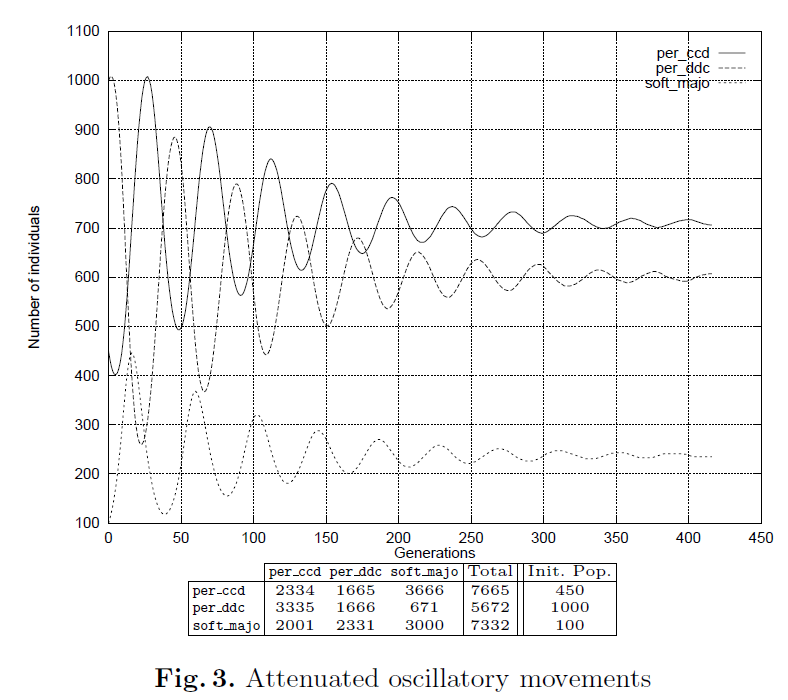
\includegraphics[width=\linewidth]{Figures Fitness Dynamics/3.png}
        \caption{Θεωρητικό αποτέλεσμα από προηγούμενη δημοσίευση. \textit{Πηγή:} \protect\cite{mathieu1999}}
        \label{fig:fig_fit_3_a}
    \end{subfigure}
    \hfill
    \begin{subfigure}[b]{0.5\linewidth}
        \centering
        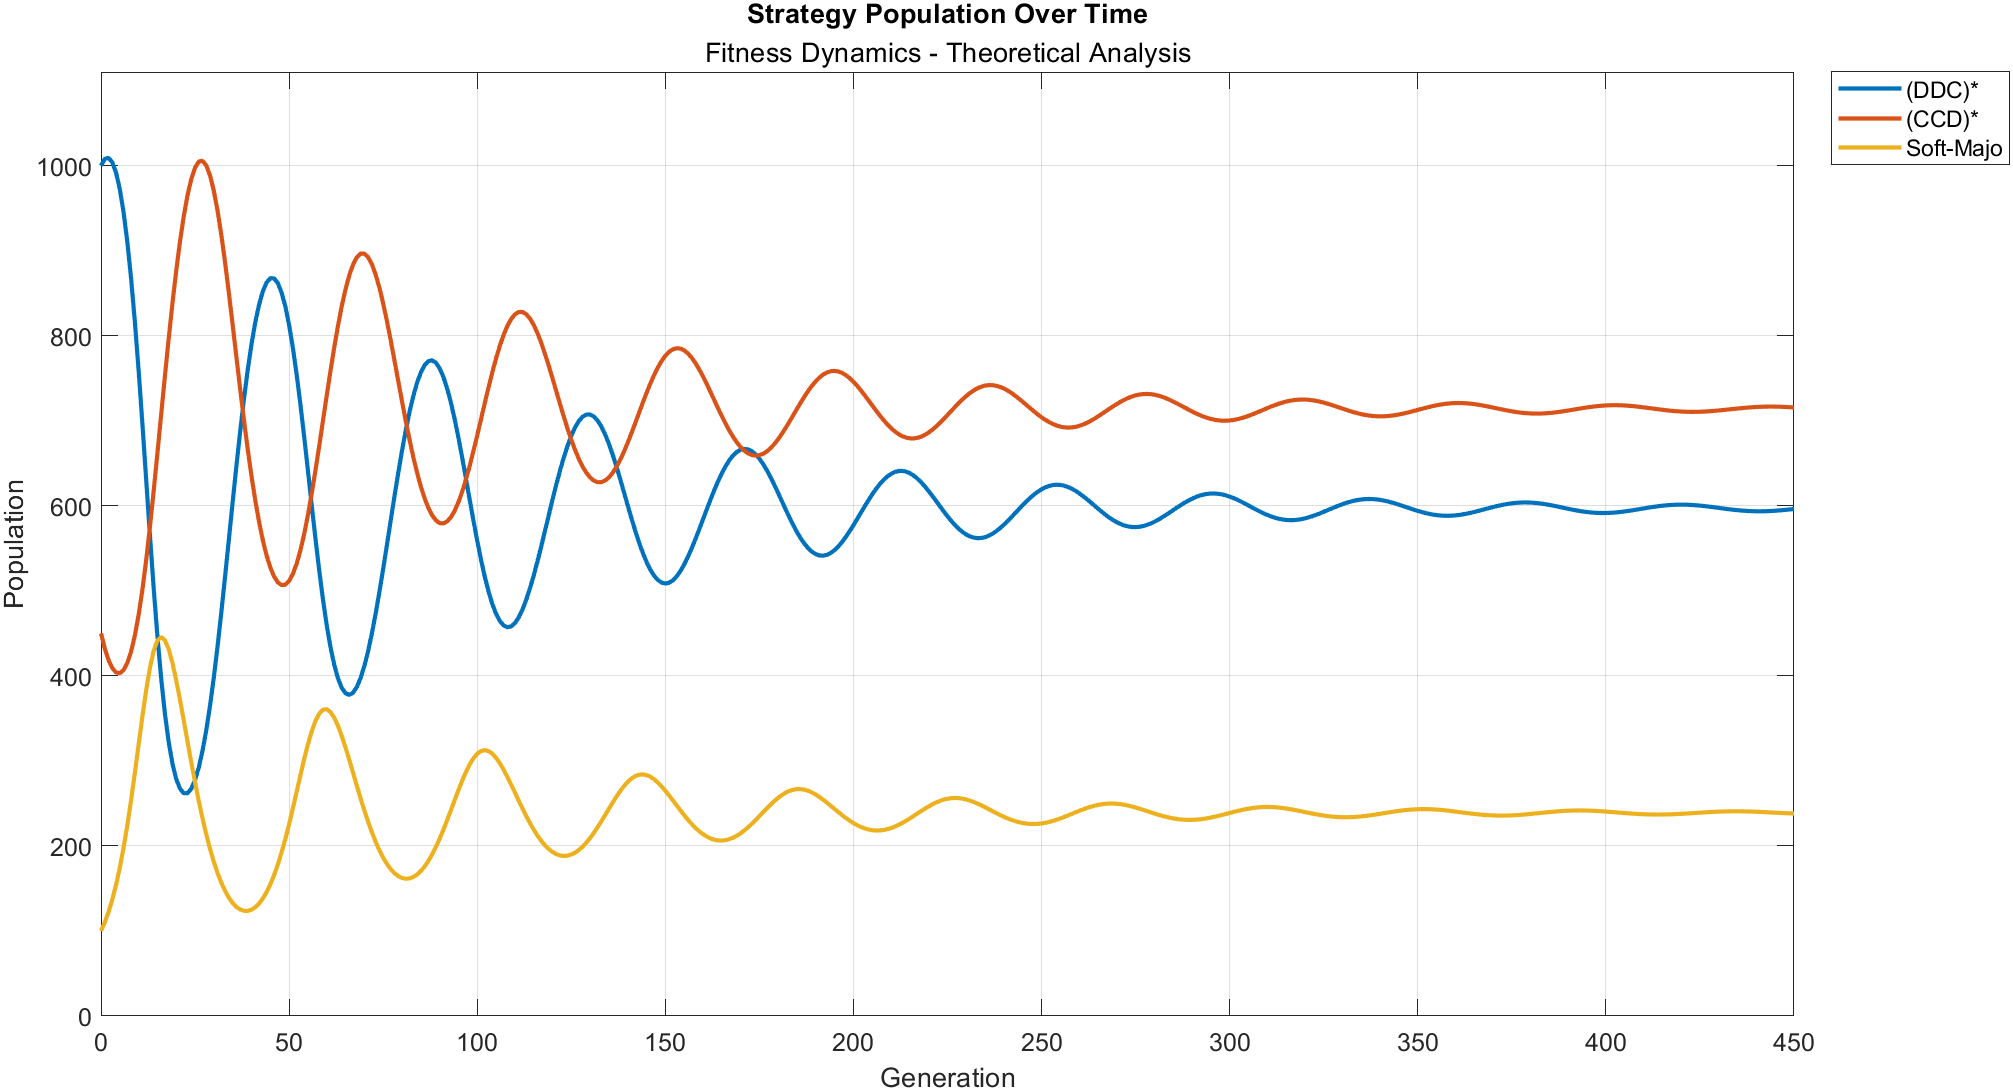
\includegraphics[width=\linewidth]{Figures Fitness Dynamics/example3.png}
        \caption{Θεωρητικό εξελικτικό πρωτάθλημα}
        \label{fig:fig_fit_3_b}
    \end{subfigure}
    \hfill
    \begin{subfigure}[b]{0.5\linewidth}
        \centering
        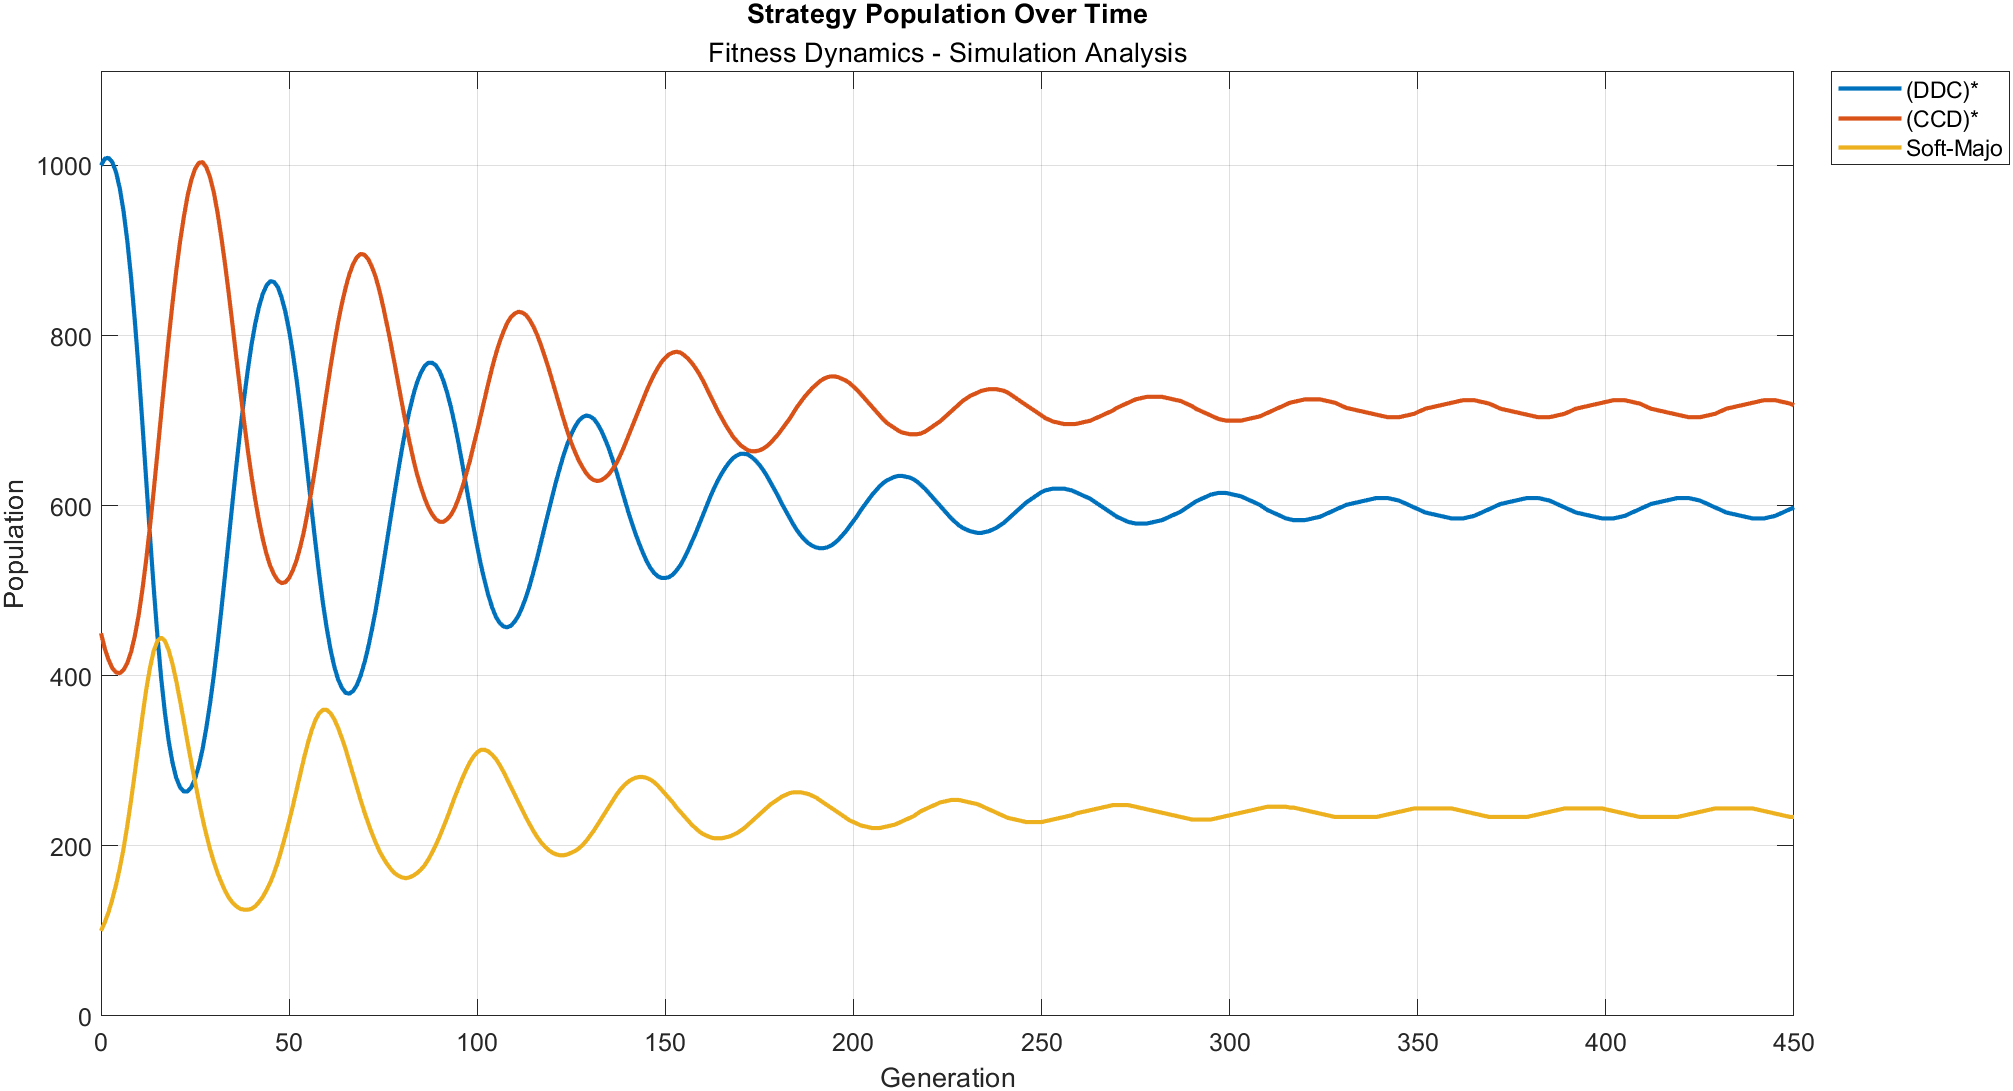
\includegraphics[width=\linewidth]{Figures Fitness Dynamics/example3-sim.png}
        \caption{Προσομοίωση εξελικτικού πρωταθλήματος}
        \label{fig:fig_fit_3_c}
    \end{subfigure}

    \caption{Αποτελέσματα πειράματος 3 - \foreignlanguage{english}{Script: example3.m}}
    \label{fig:fig_fit_3}
\end{figure}


\subsubsection{Εμφάνιση περιοδικών κινήσεων}
Στο Σχήμα \ref{fig:fig_fit_4} παρουσιάζονται τα αποτελέσματα του εξελικτικού πρωταθλήματος για τις στρατηγικές \foreignlanguage{english}{per\_ccd, per\_ddc} και \foreignlanguage{english}{soft\_majo} με αρχικούς πληθυσμούς 300, 200 και 100 αντίστοιχα. Παρατηρούμε ότι σε όλα τα αποτελέσματα παρουσιάζεται μια ταλάντωση. Η προσομοίωση συγκλίνει πλήρως, όπως φαίνεται στο ενδεικτικό γράφημα \ref{fig:fig_fit_4_a}, παρουσιάζοντας περιοδική ταλάντωση καθ’ όλη τη διάρκεια του πρωταθλήματος. Στη θεωρητική ανάλυση, το αντίστοιχο γράφημα εμφανίζει εξασθενημένη ταλάντωση, η οποία εξαλείφεται μετά την 400ή γενιά, οδηγώντας σε σταθεροποίηση των πληθυσμών των στρατηγικών.

\begin{figure}[htbp]
    \centering

    \begin{subfigure}[b]{0.5\linewidth}
        \centering
        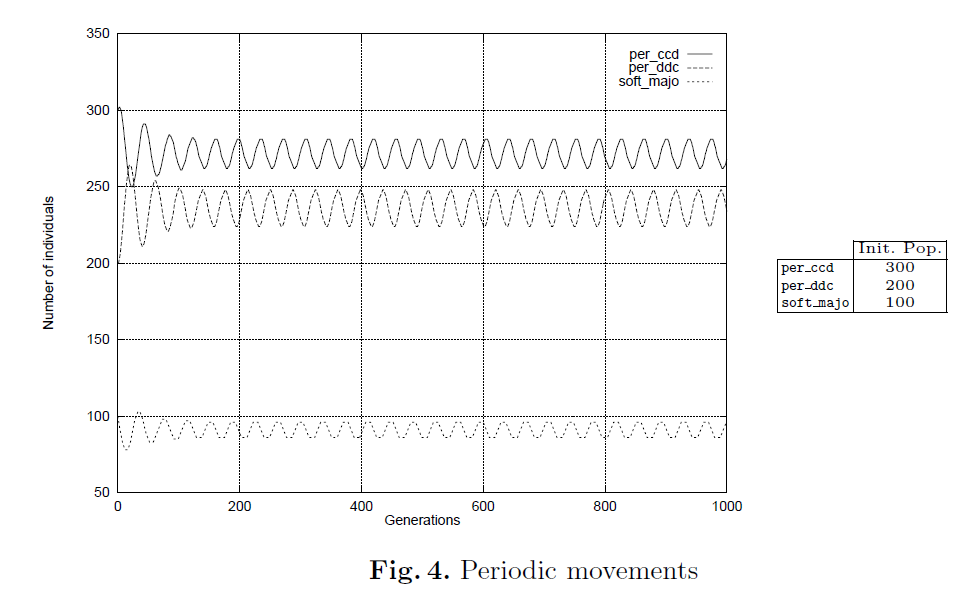
\includegraphics[width=\linewidth]{Figures Fitness Dynamics/4.png}
        \caption{Θεωρητικό αποτέλεσμα από προηγούμενη δημοσίευση. \textit{Πηγή:} \protect\cite{mathieu1999}}
        \label{fig:fig_fit_4_a}
    \end{subfigure}
    \hfill
    \begin{subfigure}[b]{0.5\linewidth}
        \centering
        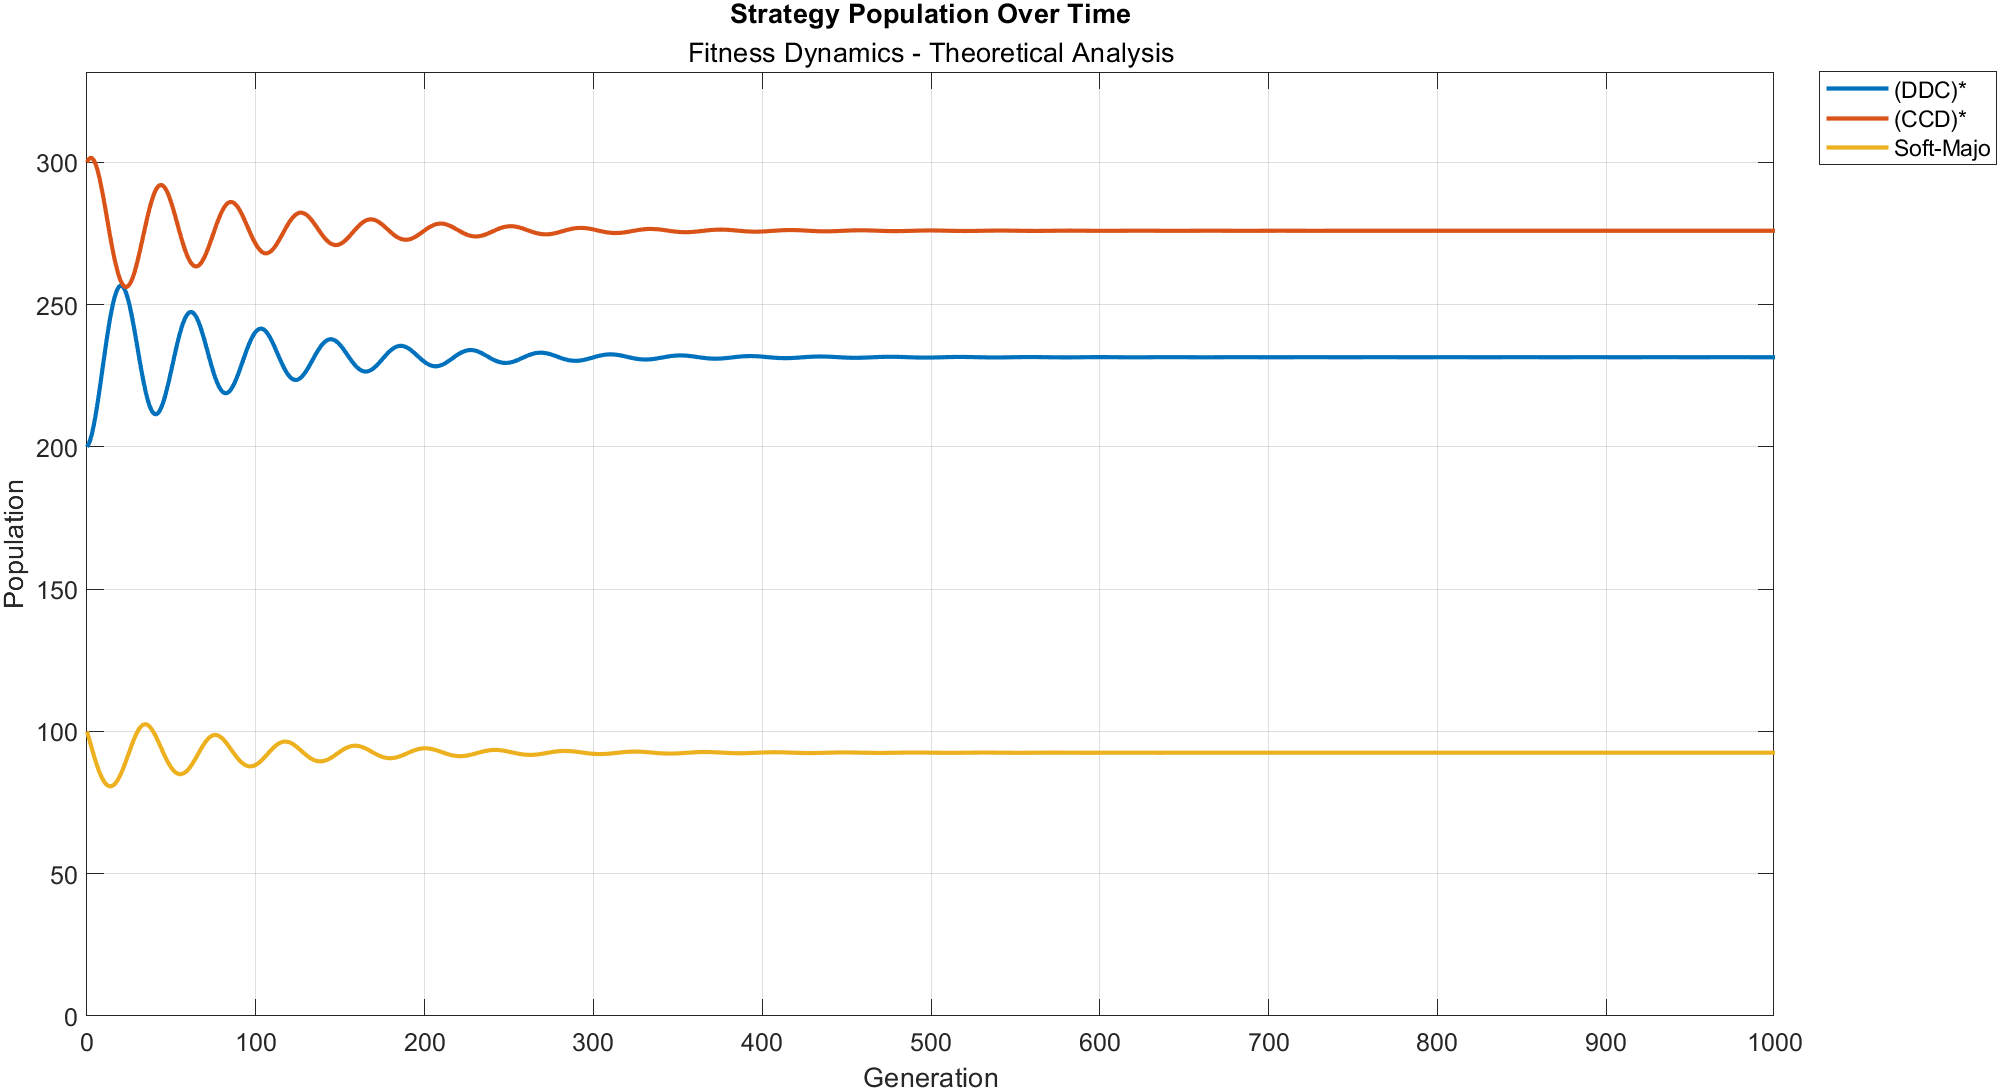
\includegraphics[width=\linewidth]{Figures Fitness Dynamics/example4.png}
        \caption{Θεωρητικό εξελικτικό πρωτάθλημα}
        \label{fig:fig_fit_4_b}
    \end{subfigure}
    \hfill
    \begin{subfigure}[b]{0.5\linewidth}
        \centering
        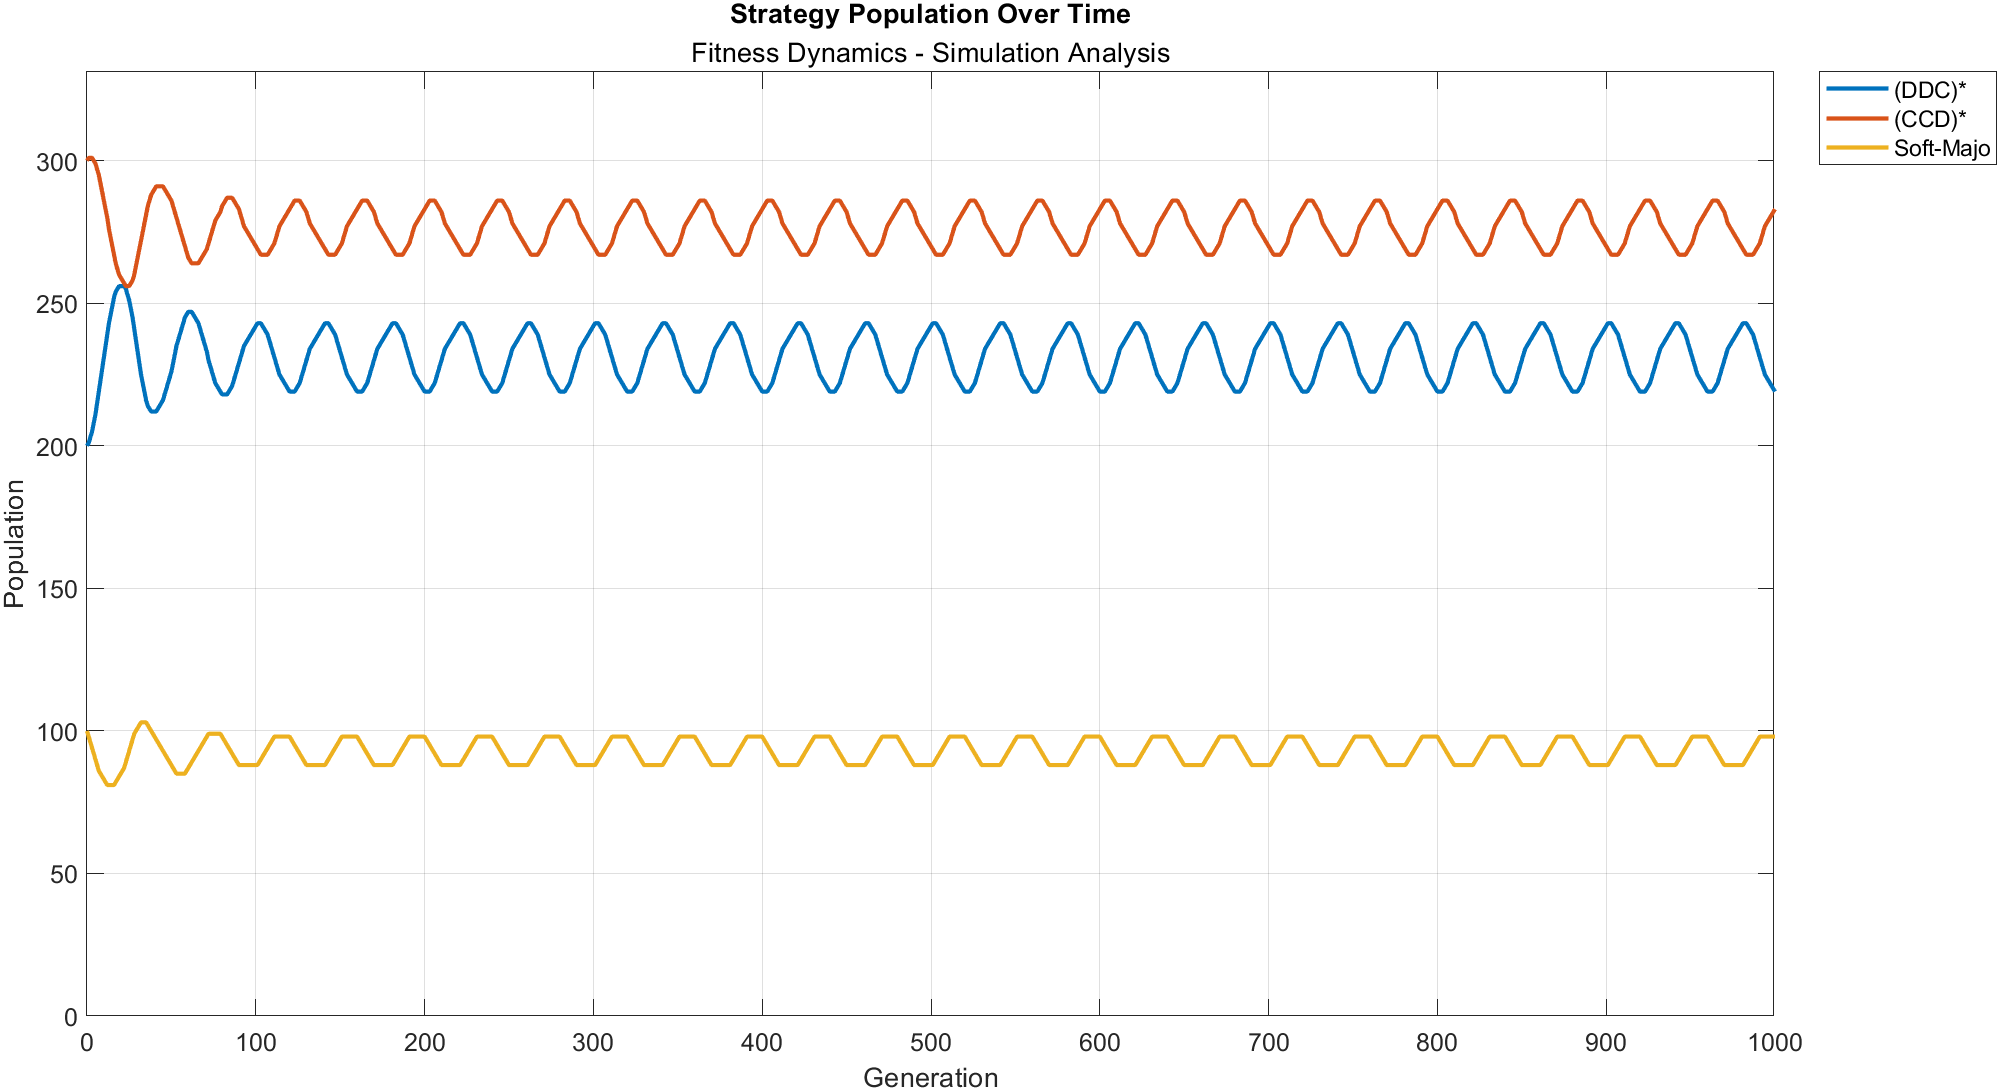
\includegraphics[width=\linewidth]{Figures Fitness Dynamics/example4-sim.png}
        \caption{Προσομοίωση εξελικτικού πρωταθλήματος}
        \label{fig:fig_fit_4_c}
    \end{subfigure}

    \caption{Αποτελέσματα πειράματος 4 - \foreignlanguage{english}{Script: example4.m}}
    \label{fig:fig_fit_4}
\end{figure}

\subsubsection{Εμφάνιση αυξανόμενων ταλάντωσεων}
Στο Σχήμα \ref{fig:fig_fit_5} παρουσιάζονται τα αποτελέσματα του εξελικτικού πρωταθλήματος για τις στρατηγικές \foreignlanguage{english}{per\_ccd}, \foreignlanguage{english}{per\_ddc} και \foreignlanguage{english}{soft\_majo}, με αρχικούς πληθυσμούς 300, 400 και 200 αντίστοιχα. Η θεωρητική ανάλυση (βλ. Σχήμα \ref{fig:fig_fit_5_c}) από την δημοσίευση δείχνει ότι η εξέλιξη των στρατηγικών ακολουθεί τη μορφή αυξανόμενης ταλάντωσης, καθώς οι διακυμάνσεις ενισχύονται σταδιακά με την πάροδο των γενεών. Αντιθέτως, στα αποτελέσματα της προσομοίωσης παρατηρείται φθίνουσα ταλάντωση, η οποία εξασθενεί και τελικά σταθεροποιείται μετά από έναν αριθμό γενεών.

\begin{figure}[htbp]
    \centering

    \begin{subfigure}[b]{0.5\linewidth}
        \centering
        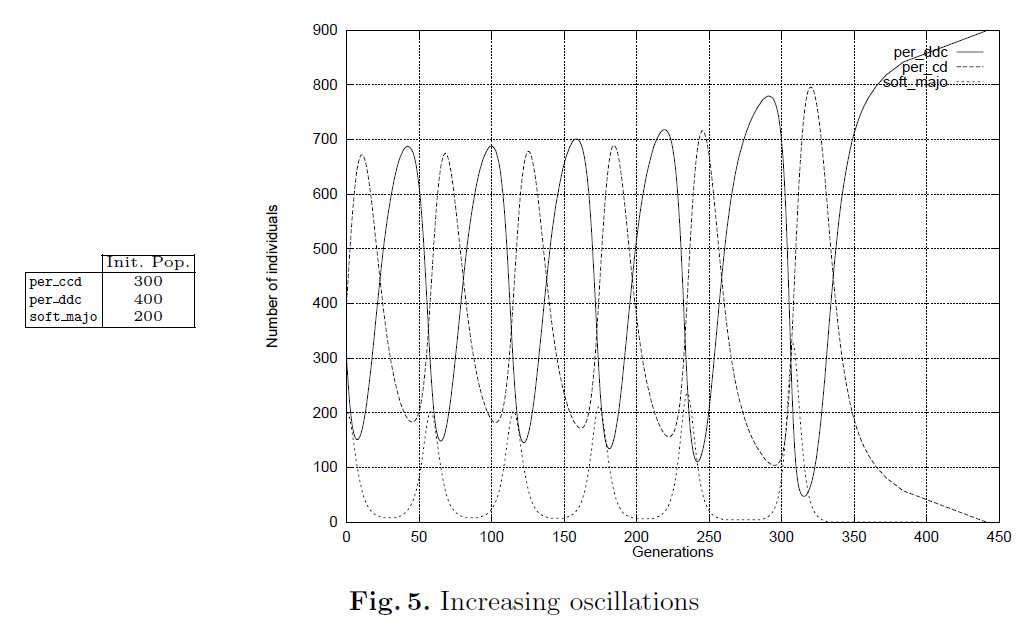
\includegraphics[width=\linewidth]{Figures Fitness Dynamics/5.png}
        \caption{Θεωρητικό αποτέλεσμα από προηγούμενη δημοσίευση. \textit{Πηγή:} \protect\cite{mathieu1999}}
        \label{fig:fig_fit_5_a}
    \end{subfigure}
    \hfill
    \begin{subfigure}[b]{0.5\linewidth}
        \centering
        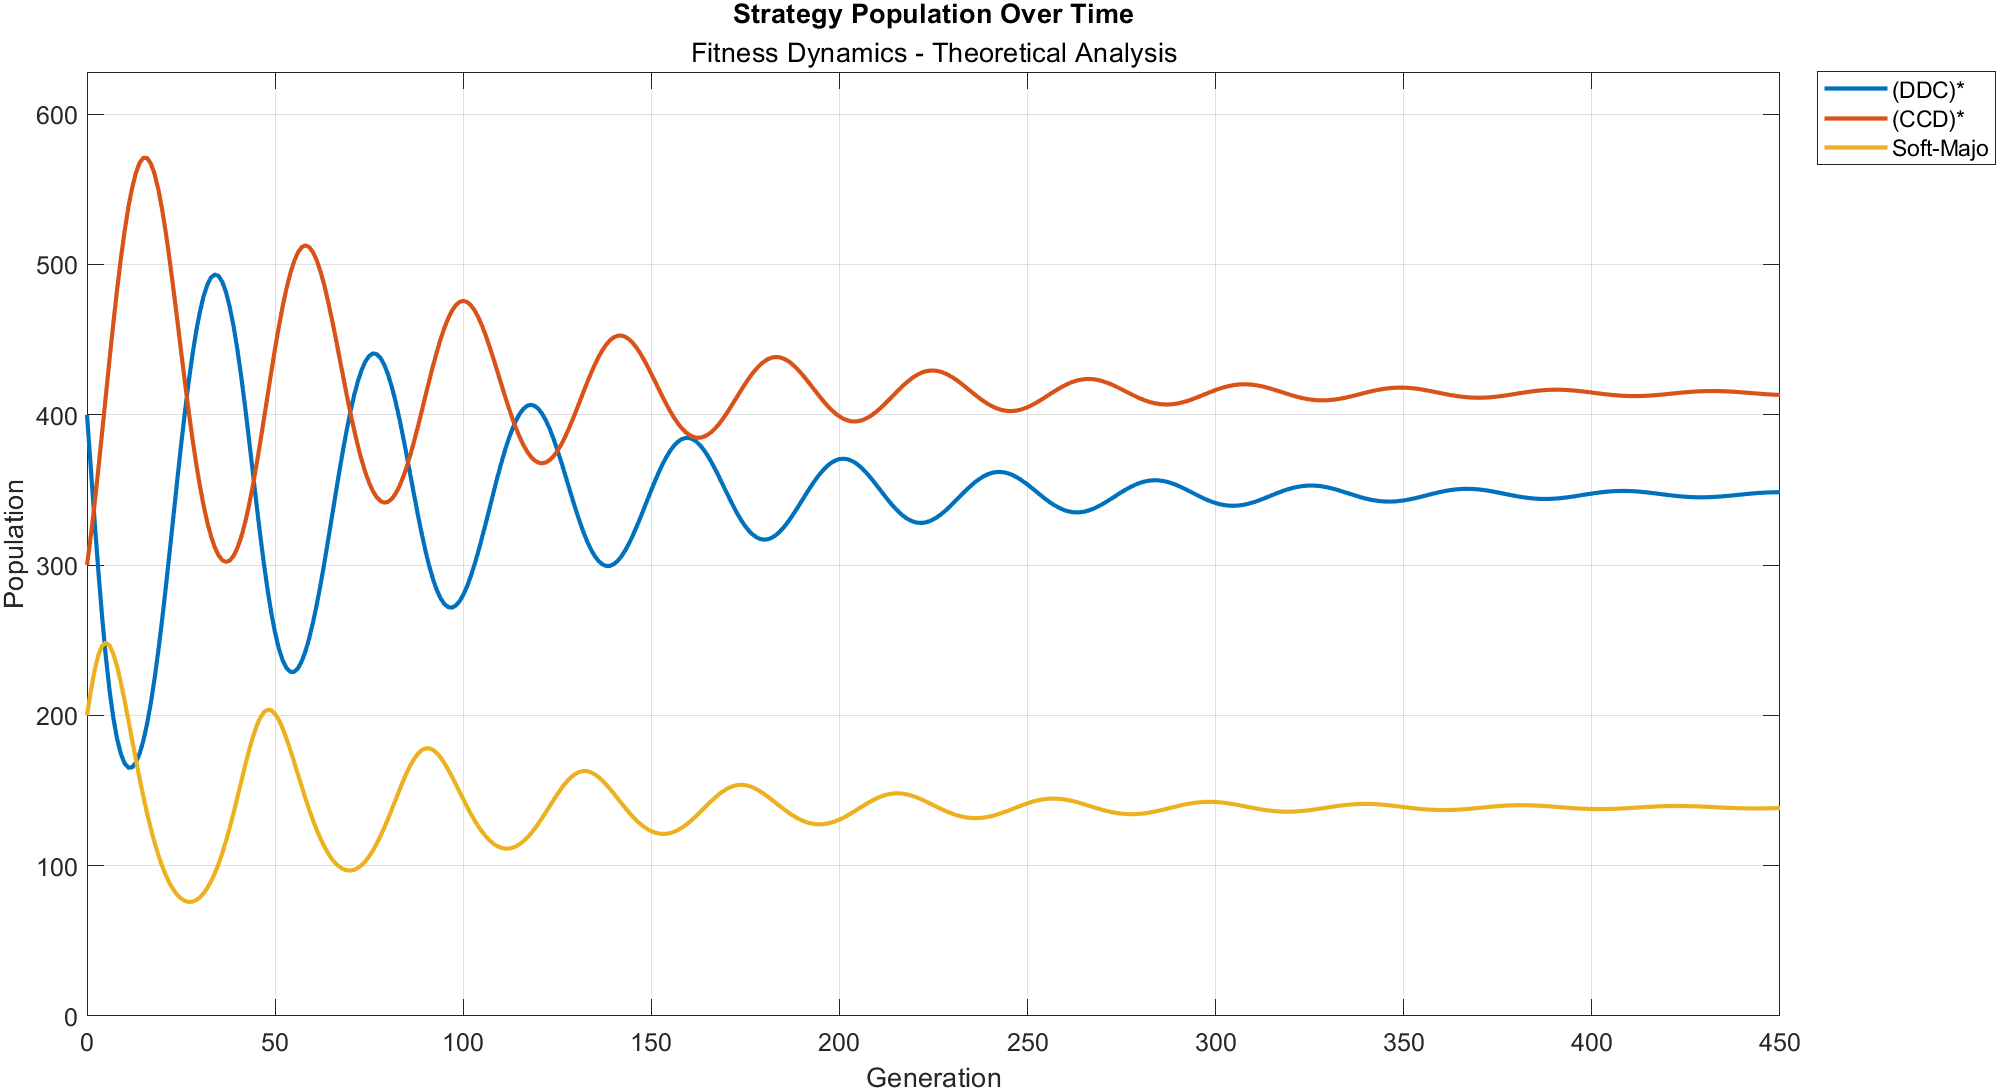
\includegraphics[width=\linewidth]{Figures Fitness Dynamics/example5.png}
        \caption{Θεωρητικό εξελικτικό πρωτάθλημα}
        \label{fig:fig_fit_5_b}
    \end{subfigure}
    \hfill
    \begin{subfigure}[b]{0.5\linewidth}
        \centering
        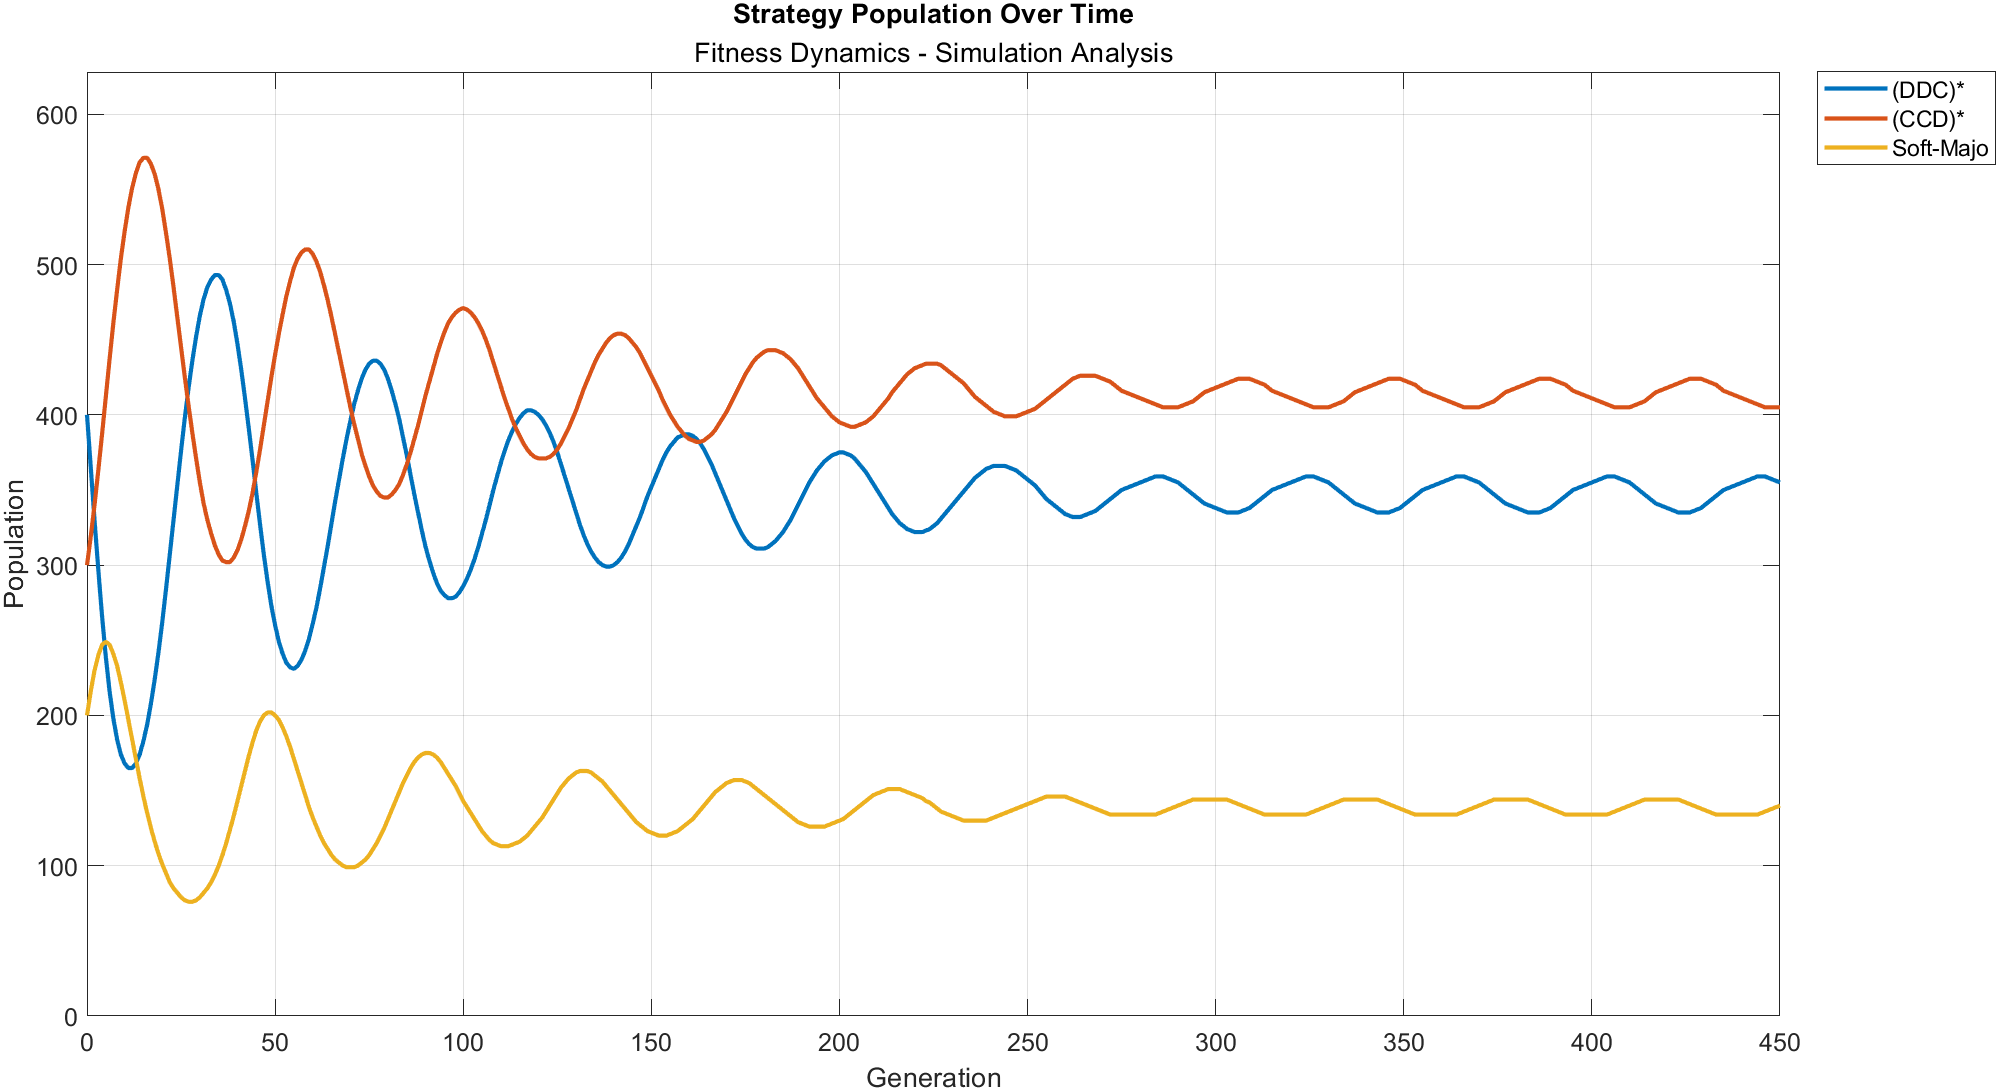
\includegraphics[width=\linewidth]{Figures Fitness Dynamics/example5-sim.png}
        \caption{Προσομοίωση εξελικτικού πρωταθλήματος}
        \label{fig:fig_fit_5_c}
    \end{subfigure}

    \caption{Αποτελέσματα πειράματος 5 - \foreignlanguage{english}{Script: example5.m}}
    \label{fig:fig_fit_5}
\end{figure}

\subsubsection{Εμφάνιση χαοτικών ταλαντώσεων}
Στο Σχήμα \ref{fig:fig_fit_6} παρουσιάζονται τα αποτελέσματα του εξελικτικού πρωταθλήματος για τις στρατηγικές \foreignlanguage{english}{soft\_majo}, \foreignlanguage{english}{per\_ccccd} και \foreignlanguage{english}{prober}, με αρχικούς πληθυσμούς 100, 500 και 800 αντίστοιχα. Η εξέλιξη των στρατηγικών και στις τρεις περιπτώσεις φαίνεται να ακολουθούν μια παρόμοια μορφή. Στο πρώτο γράφημα παρατηρείται μια προσωρινή αναταραχή γύρω στη 140ή γενιά, η οποία όμως εξομαλύνεται κατά την περαιτέρω εξέλιξη του πρωταθλήματος. Αν και παρόμοια τάση εμφανίζεται και στα γραφήματα της προσομοίωσής μας, η αταξία είναι αισθητά πιο ήπια και περιορισμένη.

\begin{figure}[htbp]
    \centering

    \begin{subfigure}[b]{0.5\linewidth}
        \centering
        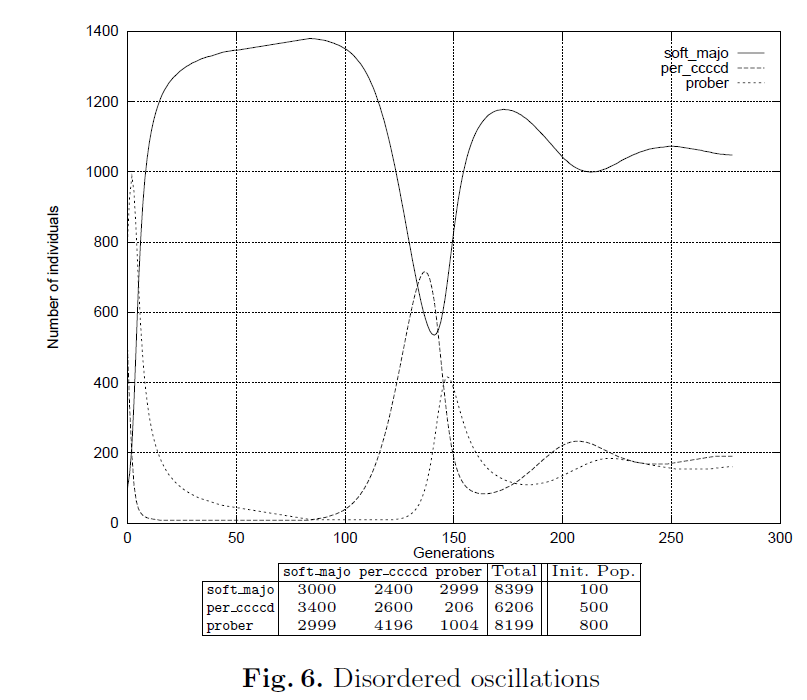
\includegraphics[width=\linewidth]{Figures Fitness Dynamics/6.png}
        \caption{Θεωρητικό αποτέλεσμα από προηγούμενη δημοσίευση. \textit{Πηγή:} \protect\cite{mathieu1999}}
        \label{fig:fig_fit_6_a}
    \end{subfigure}
    \hfill
    \begin{subfigure}[b]{0.5\linewidth}
        \centering
        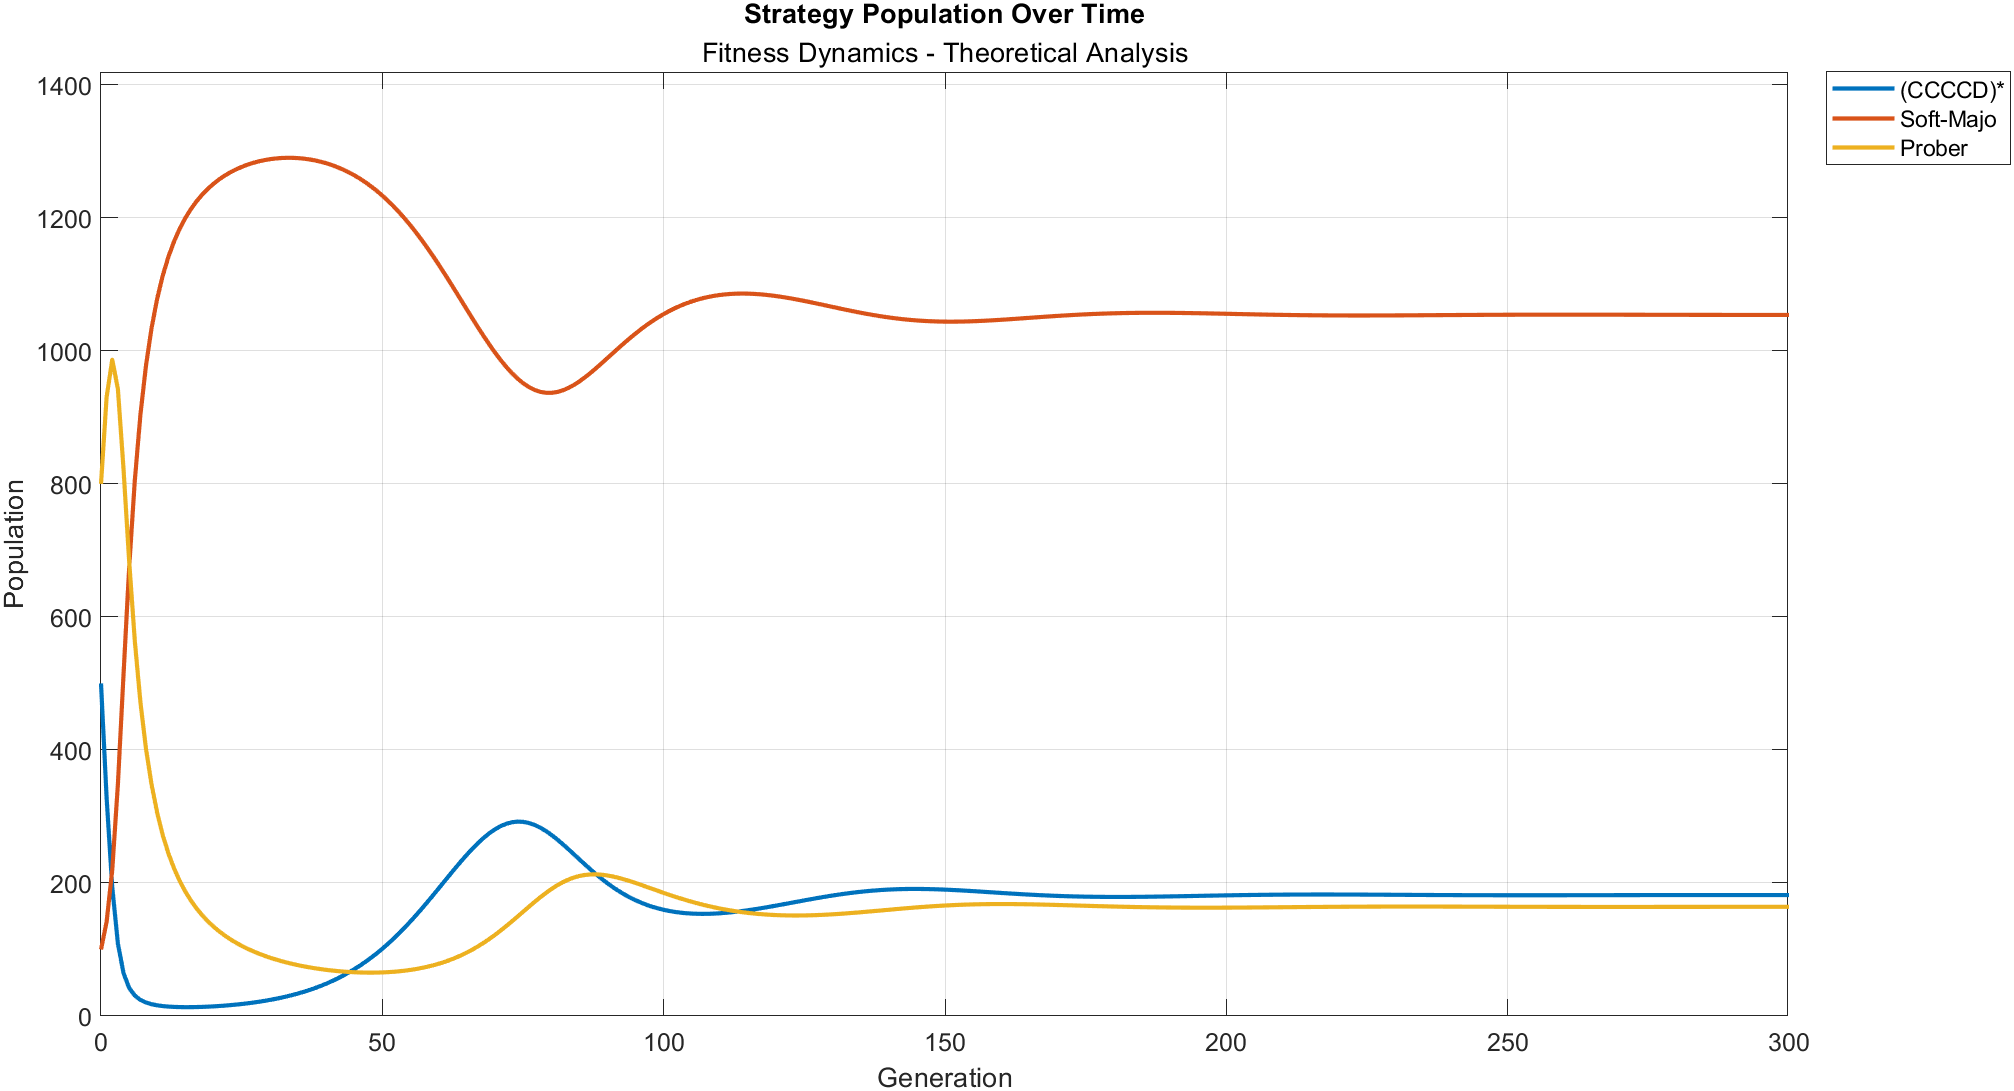
\includegraphics[width=\linewidth]{Figures Fitness Dynamics/example6.png}
        \caption{Θεωρητικό εξελικτικό πρωτάθλημα}
        \label{fig:fig_fit_6_b}
    \end{subfigure}
    \hfill
    \begin{subfigure}[b]{0.5\linewidth}
        \centering
        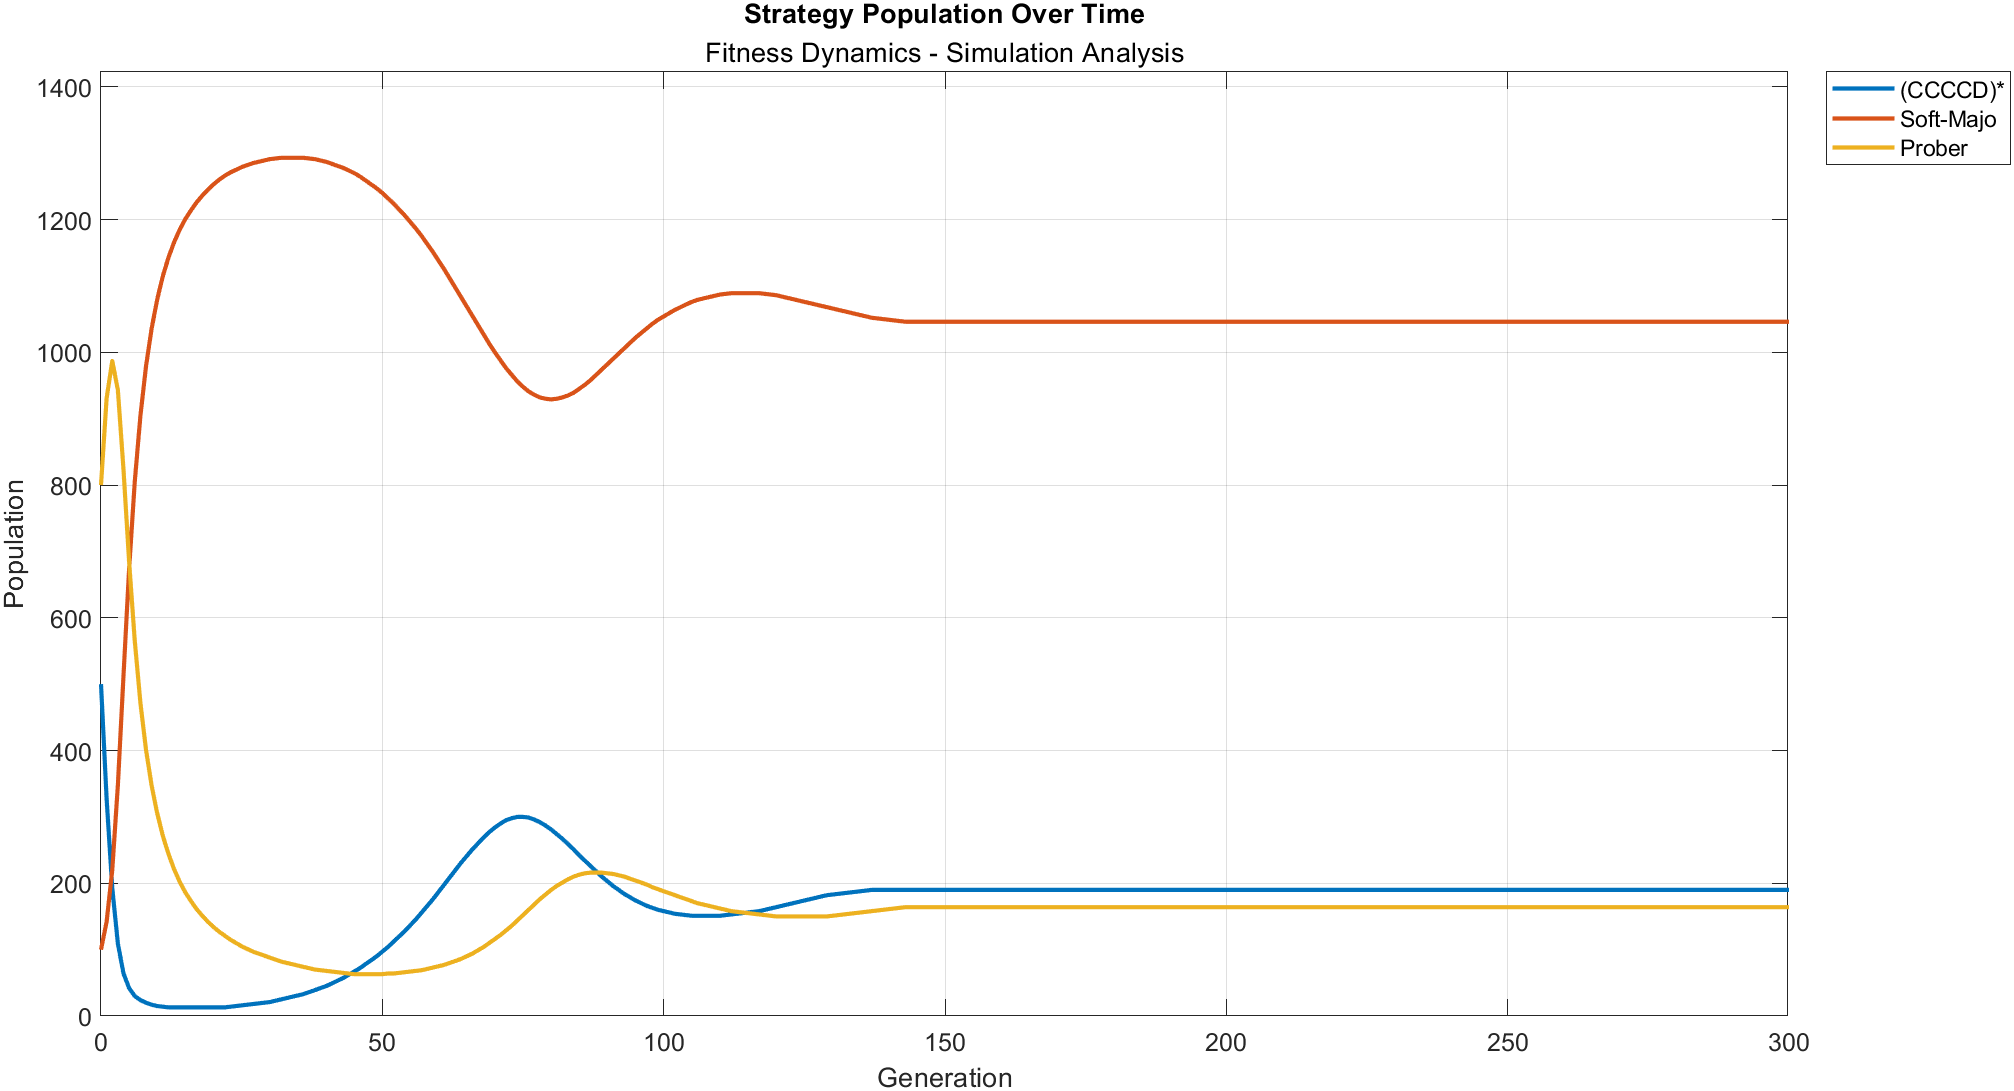
\includegraphics[width=\linewidth]{Figures Fitness Dynamics/example6-sim.png}
        \caption{Προσομοίωση εξελικτικού πρωταθλήματος}
        \label{fig:fig_fit_6_c}
    \end{subfigure}

    \caption{Αποτελέσματα πειράματος 6 - \foreignlanguage{english}{Script: example6.m}}
    \label{fig:fig_fit_6}
\end{figure}

\subsubsection{Ευαισθησία στο μέγεθος του πληθυσμού}
Για να μελετήσουμε την επίδραση του μέγεθους του αρχικού πληθυσμού στην εξέλιξη του πρωταθλήματος διεξάγουμε τα ακόλουθα δύο πειράματα, στα οποία μεταβάλλουμε τον πληθυσμό της μιας στρατηγικής.

\subsubsection*{Πρώτο πείραμα}
Στο Σχήμα \ref{fig:fig_fit_7a} παρουσιάζονται τα αποτελέσματα του εξελικτικού πρωταθλήματος για τις στρατηγικές \foreignlanguage{english}{per\_ccd, per\_ddc} και \foreignlanguage{english}{soft\_majo}, με αρχικούς πληθυσμούς 300, 244 και 100 παίκτες, ενώ στο Σχήμα \ref{fig:fig_fit_7b} παρουσιάζονται τα αποτελέσματα ίδιου πρωταθλήματος με τον πληθυσμό της \foreignlanguage{english}{per\_ddc} ρυθμισμένο στους 255 παίκτες.

Με βάση την θεωρητική ανάλυση θα περιμέναμε μια περιοδική ταλάντωση για το πρώτο πρωτάθλημα και μια σχεδόν σταθερή εξέλιξη των στρατηγικών για το δεύτερο. Όσον αφορά τα αποτελέσματα των πρσομοιώσεων μας παρατηρούμε ότι λαμβάνουμε τα ίδια αποτελέσματα ανεξαρτήτως την μεταβολή του πληθυσμού. Στην θεωρητική ανάλυση παρατηρείται μια αποσβεννύμενη ταλάντωση και στα δύο πρωταθλήματα ενώ στην προσομοίωση δεν υπάρχουν μεταβολές στον πληθυσμό των στρατηγικών. 

\begin{figure}[htbp]
    \centering

    \begin{subfigure}[b]{0.5\linewidth}
        \centering
        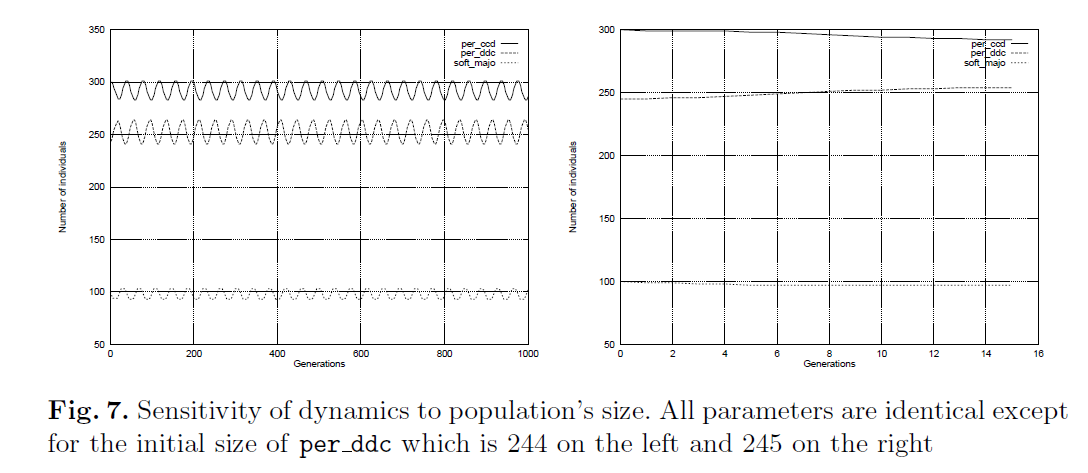
\includegraphics[width=\linewidth]{Figures Fitness Dynamics/7.png}
        \caption{Θεωρητικό αποτέλεσμα από προηγούμενη δημοσίευση. \textit{Πηγή:} \protect\cite{mathieu1999}}
        \label{fig:fig_fit_7_a}
    \end{subfigure}
    \hfill
    \begin{subfigure}[b]{0.5\linewidth}
        \centering
        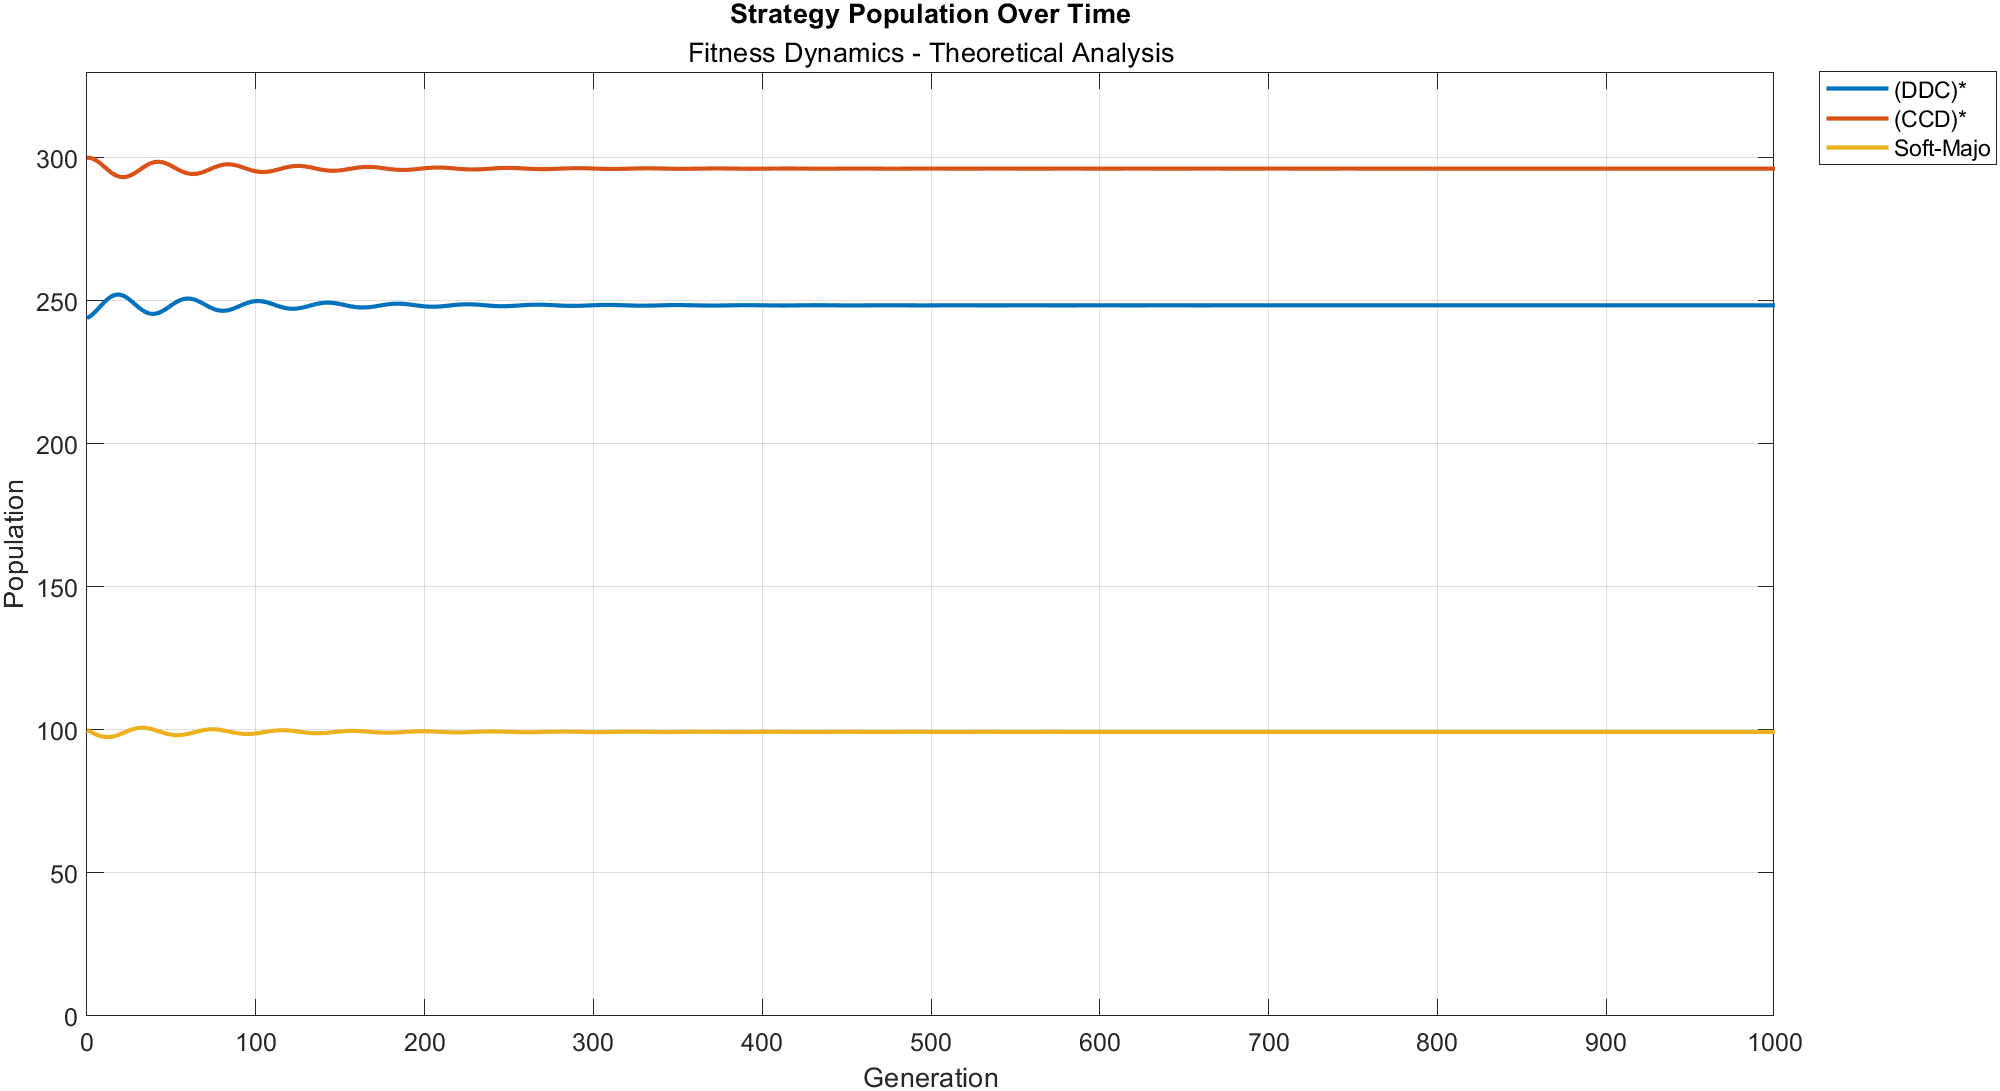
\includegraphics[width=\linewidth]{Figures Fitness Dynamics/example7a.png}
        \caption{Θεωρητικό εξελικτικό πρωτάθλημα}
        \label{fig:fig_fit_7a_b}
    \end{subfigure}
    \hfill
    \begin{subfigure}[b]{0.5\linewidth}
        \centering
        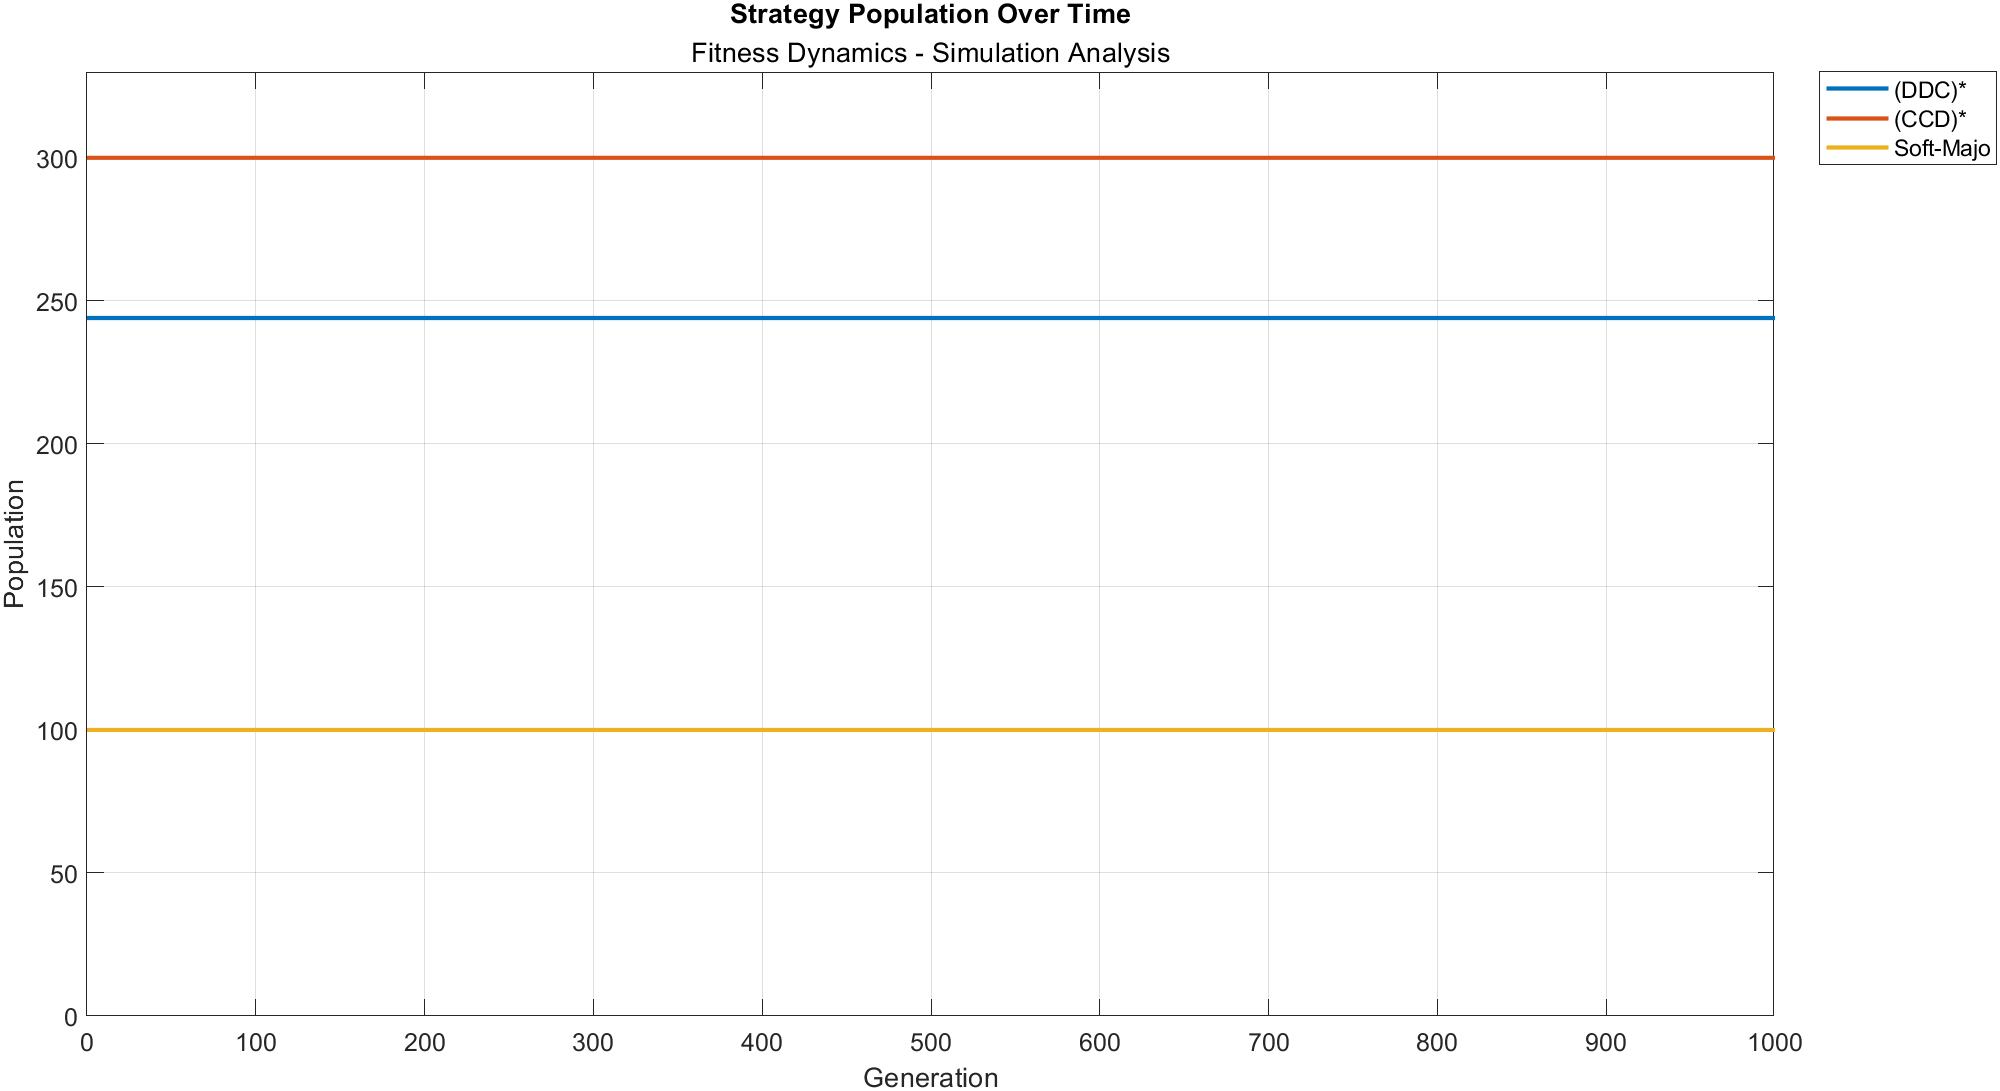
\includegraphics[width=\linewidth]{Figures Fitness Dynamics/example7a-sim.png}
        \caption{Προσομοίωση εξελικτικού πρωταθλήματος}
        \label{fig:fig_fit_7a_c}
        
    \end{subfigure}

    \caption{Αποτελέσματα πειράματος 7α - \foreignlanguage{english}{Script: example7a.m}}
    \label{fig:fig_fit_7a}
\end{figure}

\begin{figure}[htbp]
    \centering

    \begin{subfigure}[b]{0.5\linewidth}
        \centering
        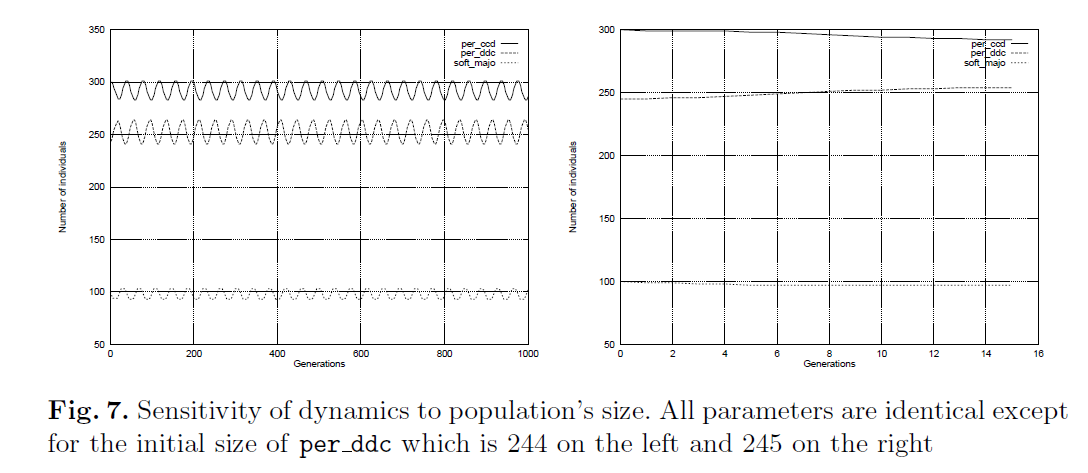
\includegraphics[width=\linewidth]{Figures Fitness Dynamics/7.png}
        \caption{Θεωρητικό αποτέλεσμα από προηγούμενη δημοσίευση. \textit{Πηγή:} \protect\cite{mathieu1999}}
    \end{subfigure}
    \hfill
    \begin{subfigure}[b]{0.5\linewidth}
        \centering
        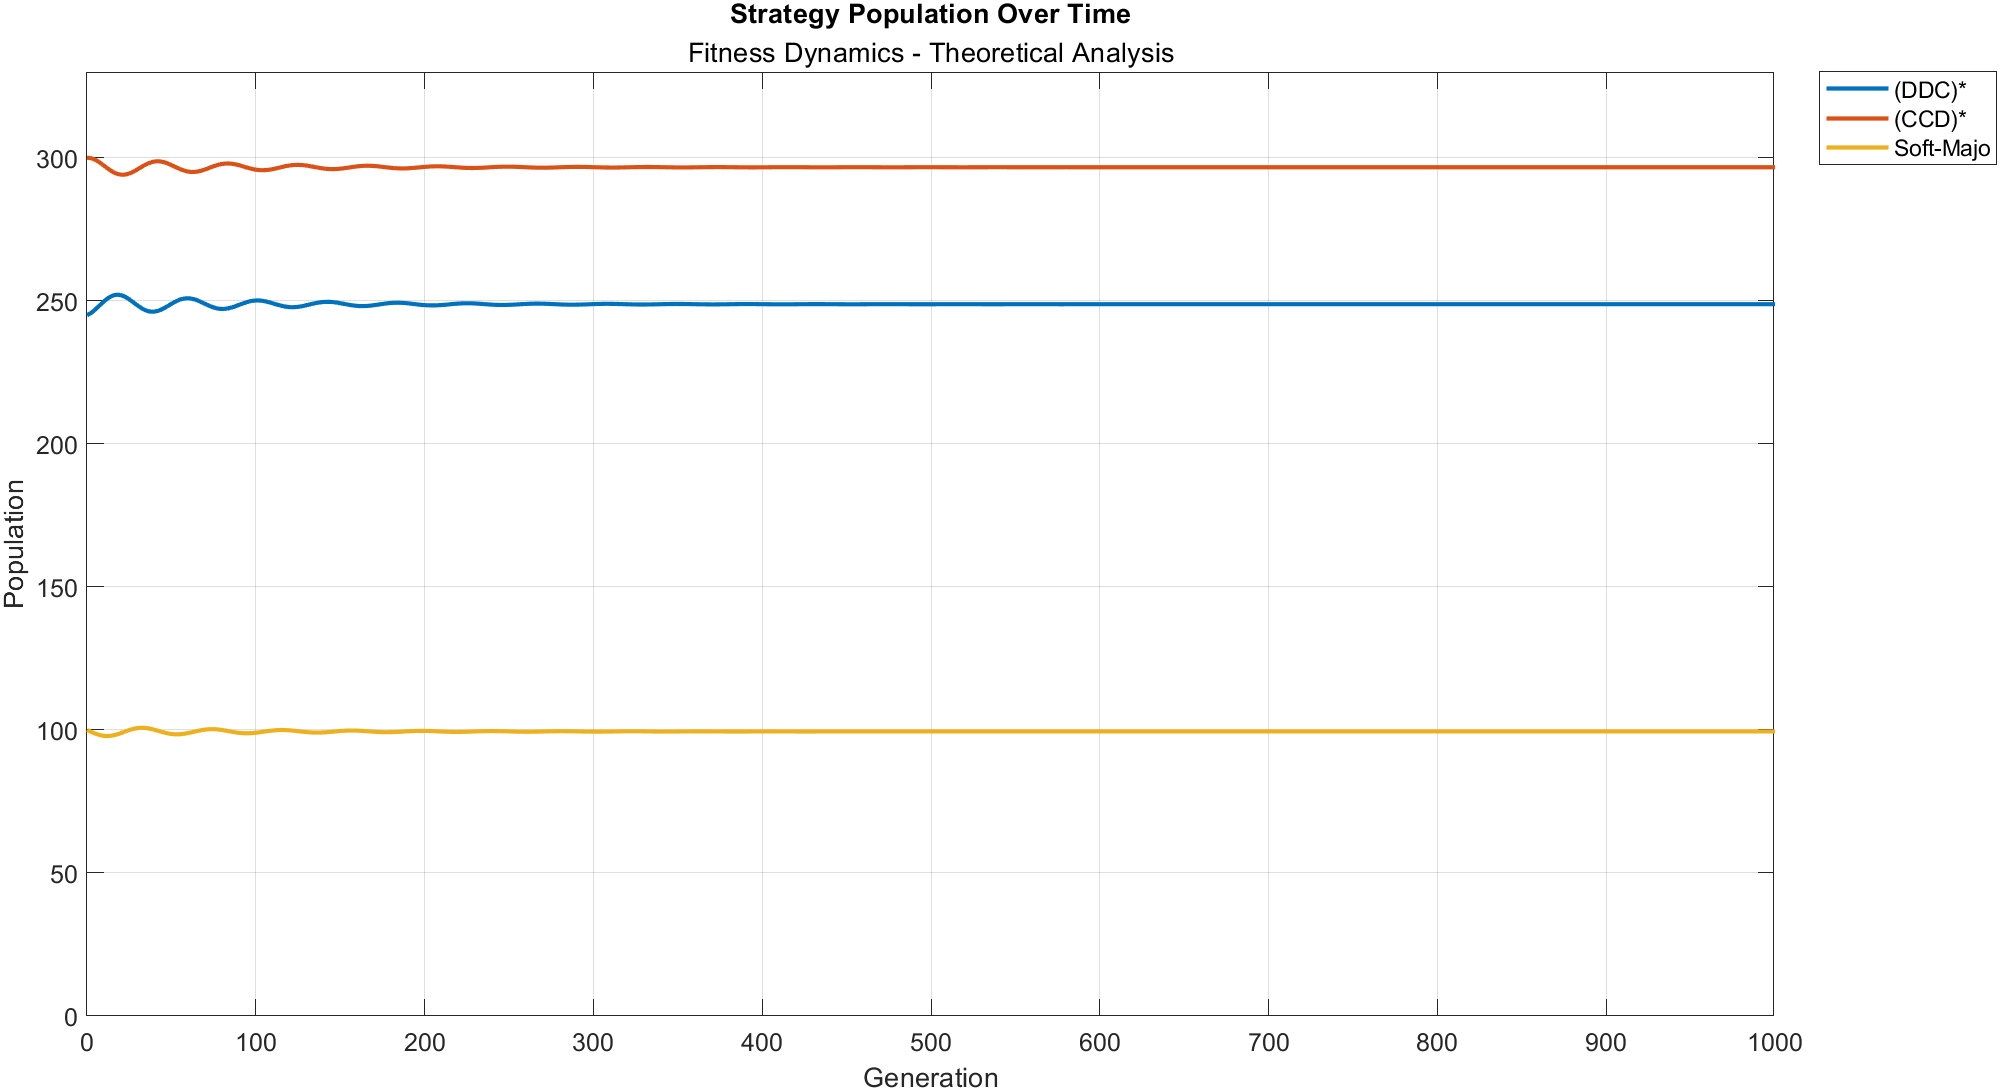
\includegraphics[width=\linewidth]{Figures Fitness Dynamics/example7b.png}
        \caption{Θεωρητικό εξελικτικό πρωτάθλημα}
        \label{fig:fig_fit_7b_b}
    \end{subfigure}
    \hfill
    \begin{subfigure}[b]{0.5\linewidth}
        \centering
        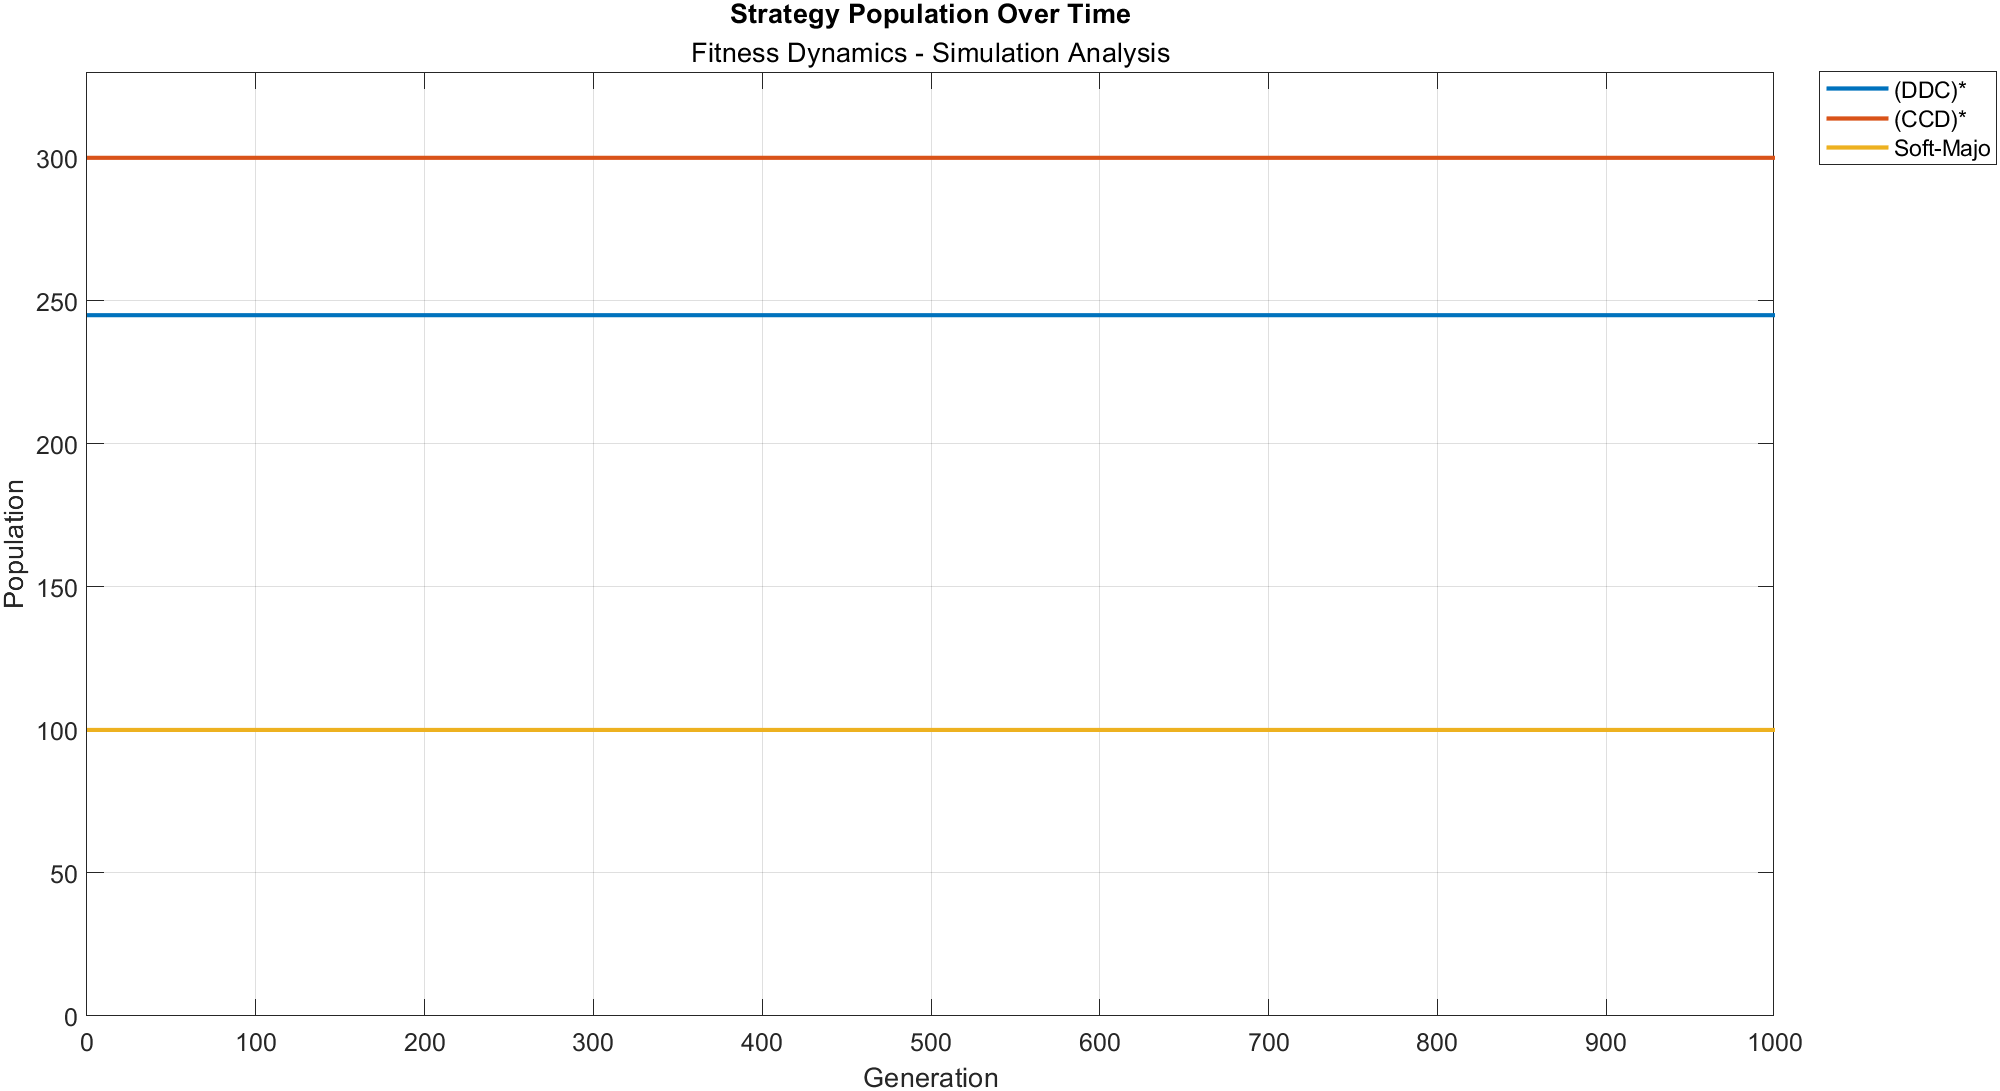
\includegraphics[width=\linewidth]{Figures Fitness Dynamics/example7b-sim.png}
        \caption{Προσομοίωση εξελικτικού πρωταθλήματος}
        \label{fig:fig_fit_7b_c}
        
    \end{subfigure}

    \caption{Αποτελέσματα πειράματος 7β - \foreignlanguage{english}{Script: example7b.m}}
    \label{fig:fig_fit_7b}
\end{figure}

\subsubsection*{Δεύτερο πείραμα}
Στο Σχήμα \ref{fig:fig_fit_8a} παρουσιάζονται τα αποτελέσματα του εξελικτικού πρωταθλήματος για τις στρατηγικές \foreignlanguage{english}{per\_ddc, per\_cd} και \foreignlanguage{english}{soft\_majo}, με αρχικούς πληθυσμούς 100, 100 και 159 αντίστοιχα ενώ στο Σχήμα \ref{fig:fig_fit_8b} ο πληθυσμός της \foreignlanguage{english}{soft\_majo} έχει αρχικοποιηθεί στους 160 παίκτες.

Στο πρώτο πρωτάθλημα που φαίνεται στα γραφήματα \ref{fig:fig_fit_8a}, παρατηρούμε ότι η εξέλιξη της προσομοίωσης του πρωταθλήματος είναι ίδια με την αναμενόμενη, ενώ η θεωρητική ανάλυση διαφέρει μετά τη 60ή γενιά, όπου η \foreignlanguage{english}{soft\_majo} αντί να χάσει όλους τους παίκτες της ανακάμπτει για μια προσωρινή περίοδο. Ωστόσο και στα τρια διαγράμματα η στρατηγική \foreignlanguage{english}{per\_ddc} αναδυκνύεται ως η επικρατέστερη.

Στο δεύτερο πρωταθλήμα \ref{fig:fig_fit_8b} παρατηρούμε ότι η μεταβολή του αρχικού πληθυσμού της \foreignlanguage{english}{soft\_majo} θα έπρεπε να συμβάλει στην ανάδειξη της \foreignlanguage{english}{per\_cd} ως καλύτερη στρατηγική. Παρόλαυτά παρατηρούμε ότι αντί οι στρατηγικές \foreignlanguage{english}{soft\_majo} και \foreignlanguage{english}{per\_ddc} να μηδενίζουν γύρω στην 25η γενιά η \foreignlanguage{english}{per\_ddc} ανακάμπτει και το πρωτάθλημα συνεχίζει να εξελίσσεται.

\begin{figure}[htbp]
    \centering

    \begin{subfigure}[b]{0.5\linewidth}
        \centering
        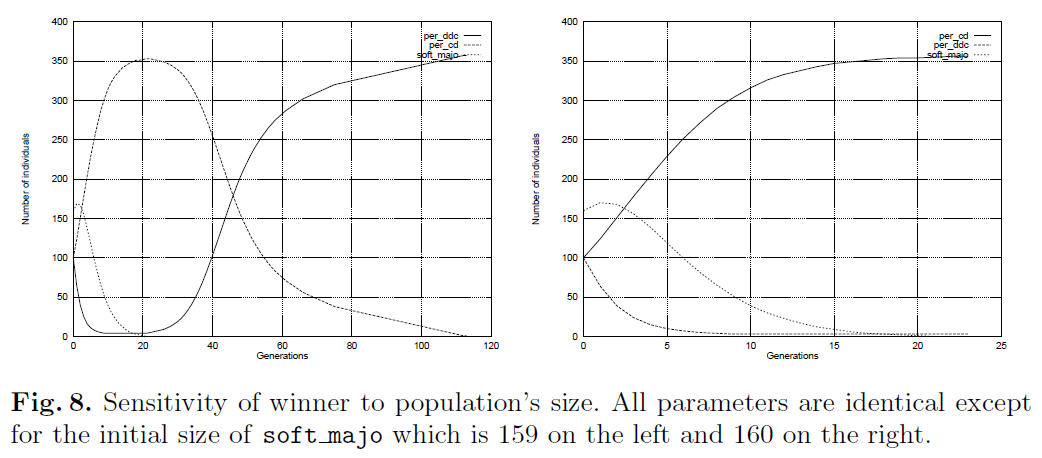
\includegraphics[width=\linewidth]{Figures Fitness Dynamics/8.png}
        \caption{Θεωρητικό αποτέλεσμα από προηγούμενη δημοσίευση. \textit{Πηγή:} \protect\cite{mathieu1999}}
        \label{fig:fig_fit_8_a}
    \end{subfigure}
    \hfill
    \begin{subfigure}[b]{0.5\linewidth}
        \centering
        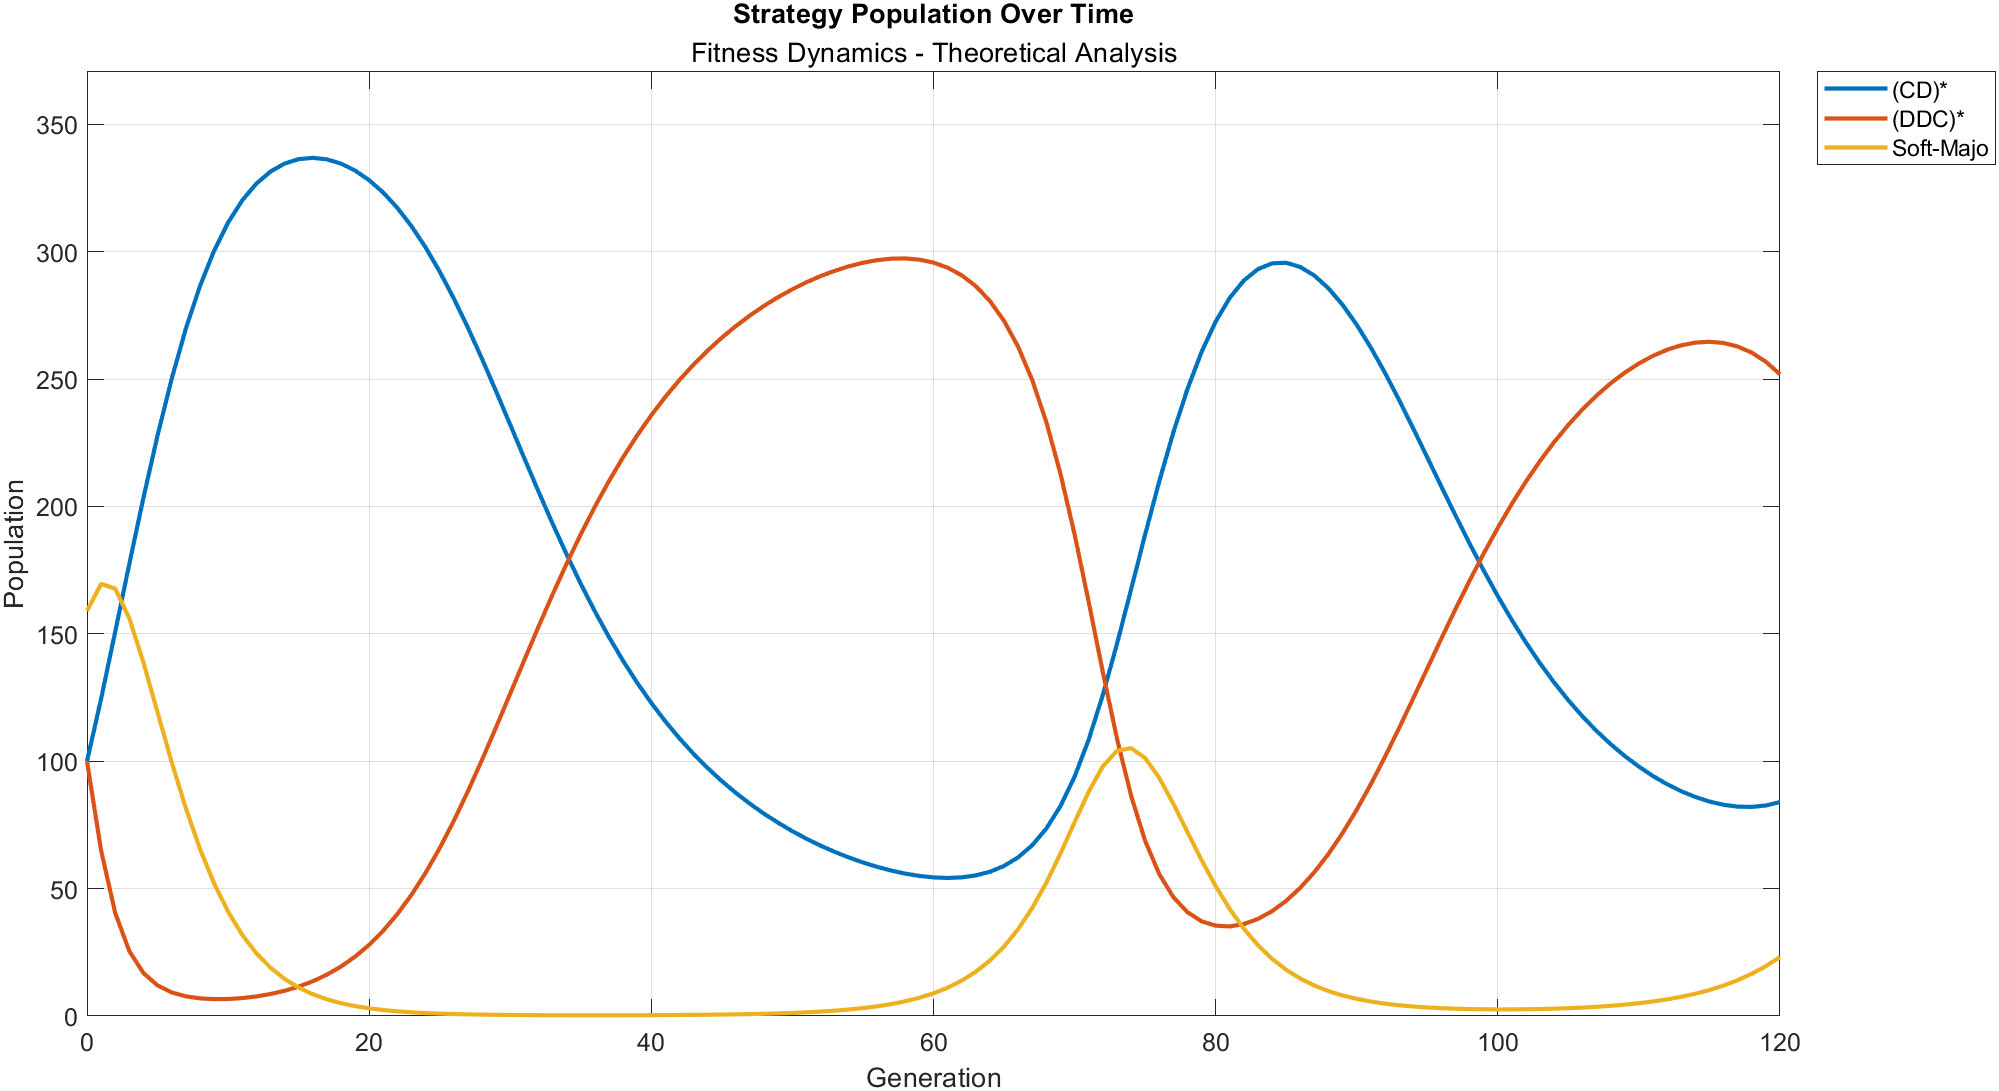
\includegraphics[width=\linewidth]{Figures Fitness Dynamics/example8a.png}
        \caption{Θεωρητικό εξελικτικό πρωτάθλημα}
        \label{fig:fig_fit_8a_b}
    \end{subfigure}
    \hfill
    \begin{subfigure}[b]{0.5\linewidth}
        \centering
        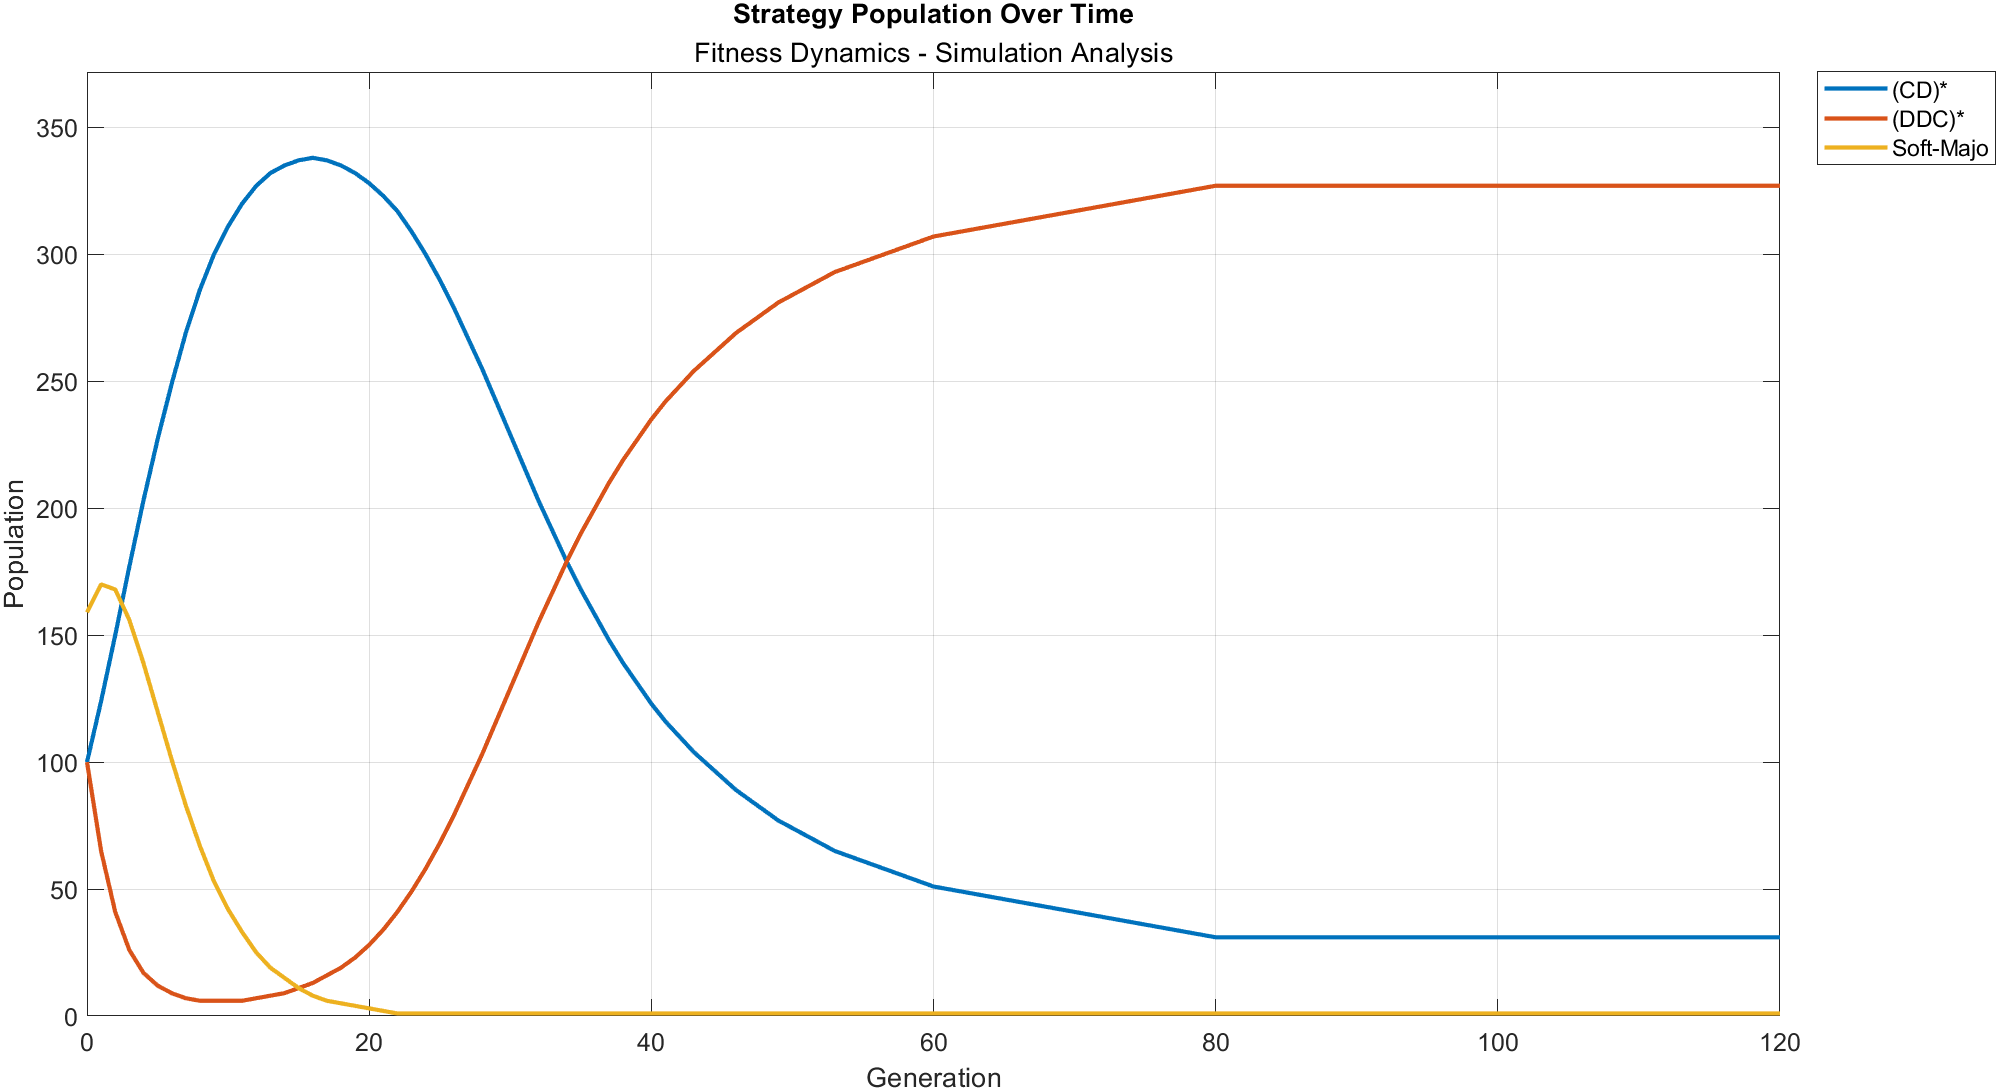
\includegraphics[width=\linewidth]{Figures Fitness Dynamics/example8a-sim.png}
        \caption{Προσομοίωση εξελικτικού πρωταθλήματος}
        \label{fig:fig_fit_8a_c}
        
    \end{subfigure}

    \caption{Αποτελέσματα πειράματος 8α - \foreignlanguage{english}{Script: example8a.m}}
    \label{fig:fig_fit_8a}
\end{figure}

\begin{figure}[htbp]
    \centering

    \begin{subfigure}[b]{0.5\linewidth}
        \centering
        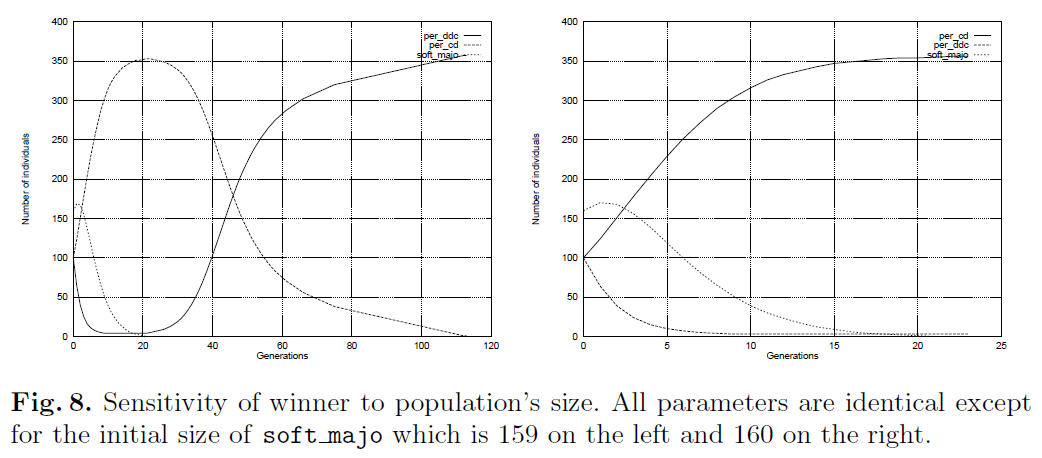
\includegraphics[width=\linewidth]{Figures Fitness Dynamics/8.png}
        \caption{Θεωρητικό αποτέλεσμα από προηγούμενη δημοσίευση. \textit{Πηγή:} \protect\cite{mathieu1999}}
    \end{subfigure}
    \hfill
    \begin{subfigure}[b]{0.5\linewidth}
        \centering
        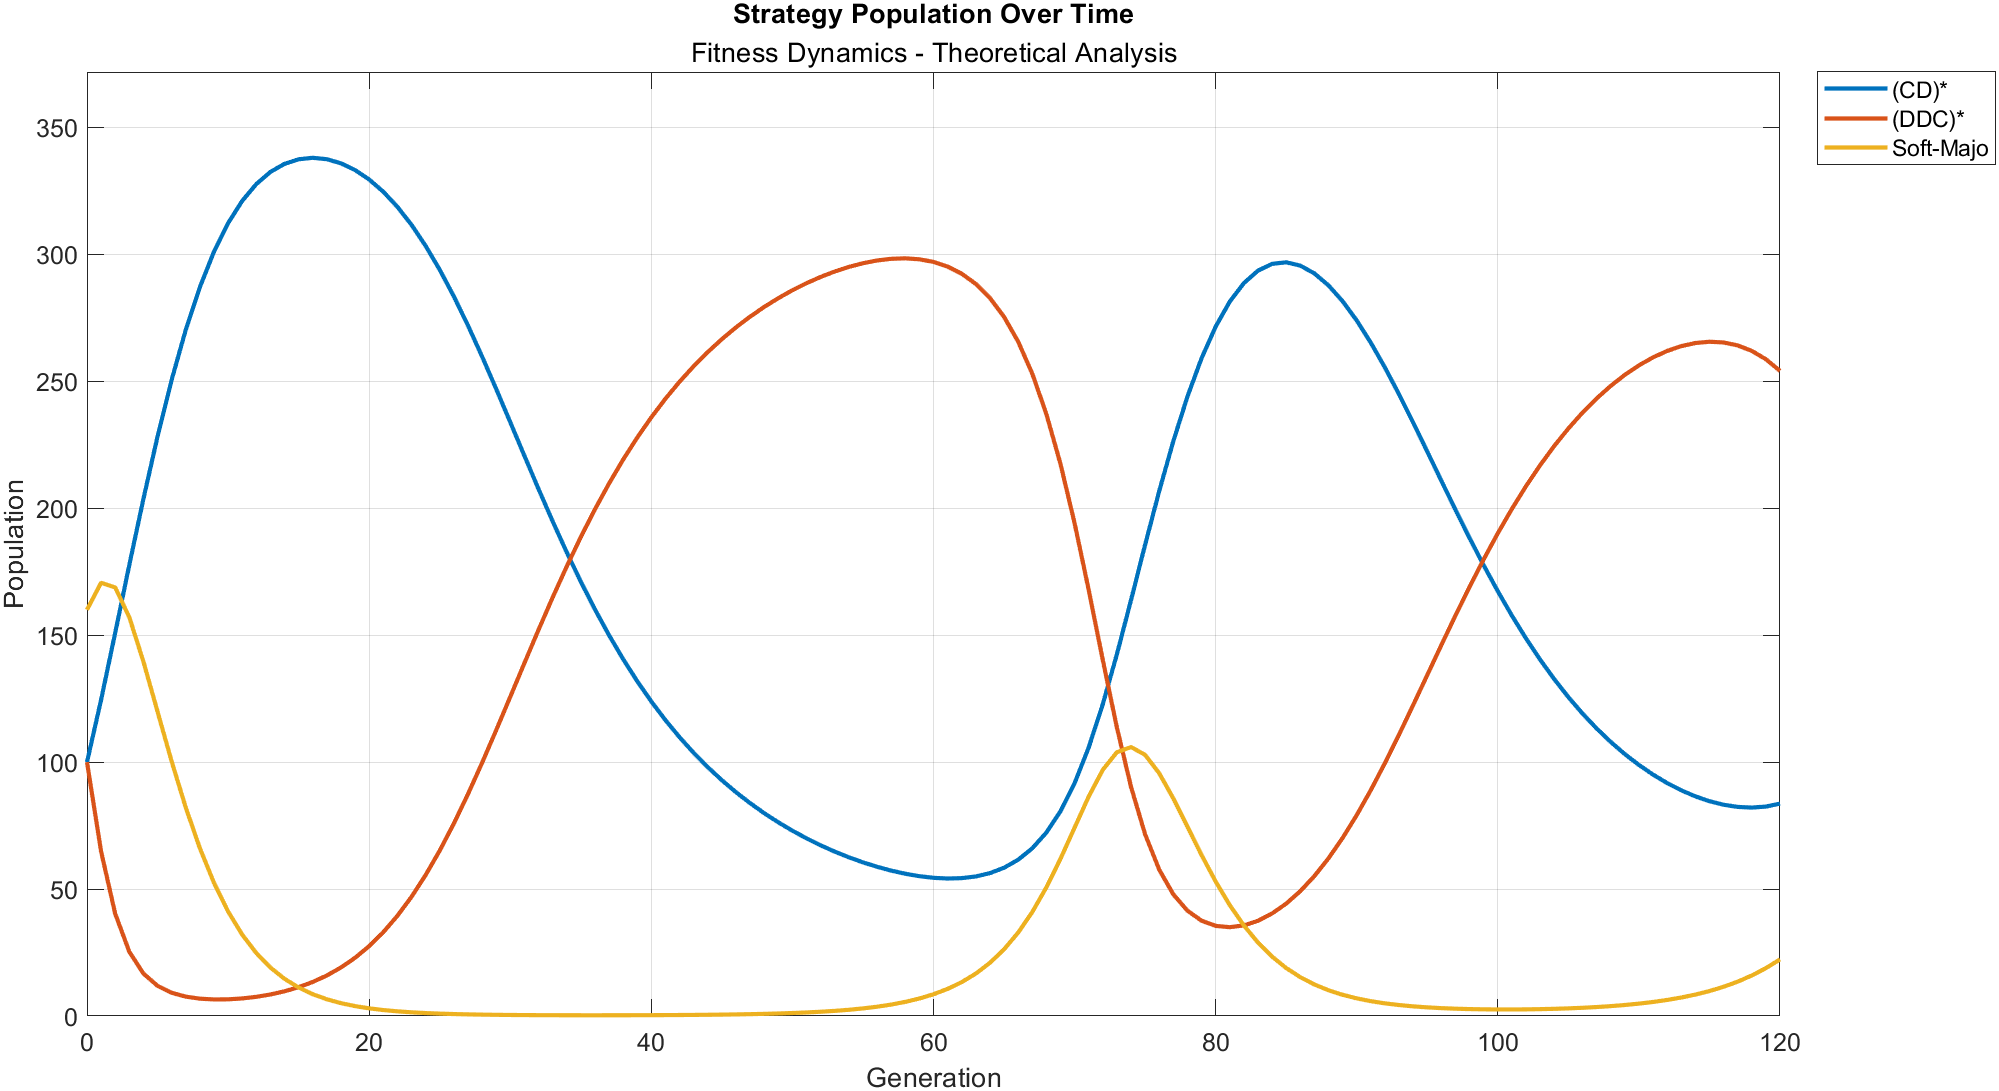
\includegraphics[width=\linewidth]{Figures Fitness Dynamics/example8b.png}
        \caption{Θεωρητικό εξελικτικό πρωτάθλημα}
        \label{fig:fig_fit_8b_b}
    \end{subfigure}
    \hfill
    \begin{subfigure}[b]{0.5\linewidth}
        \centering
        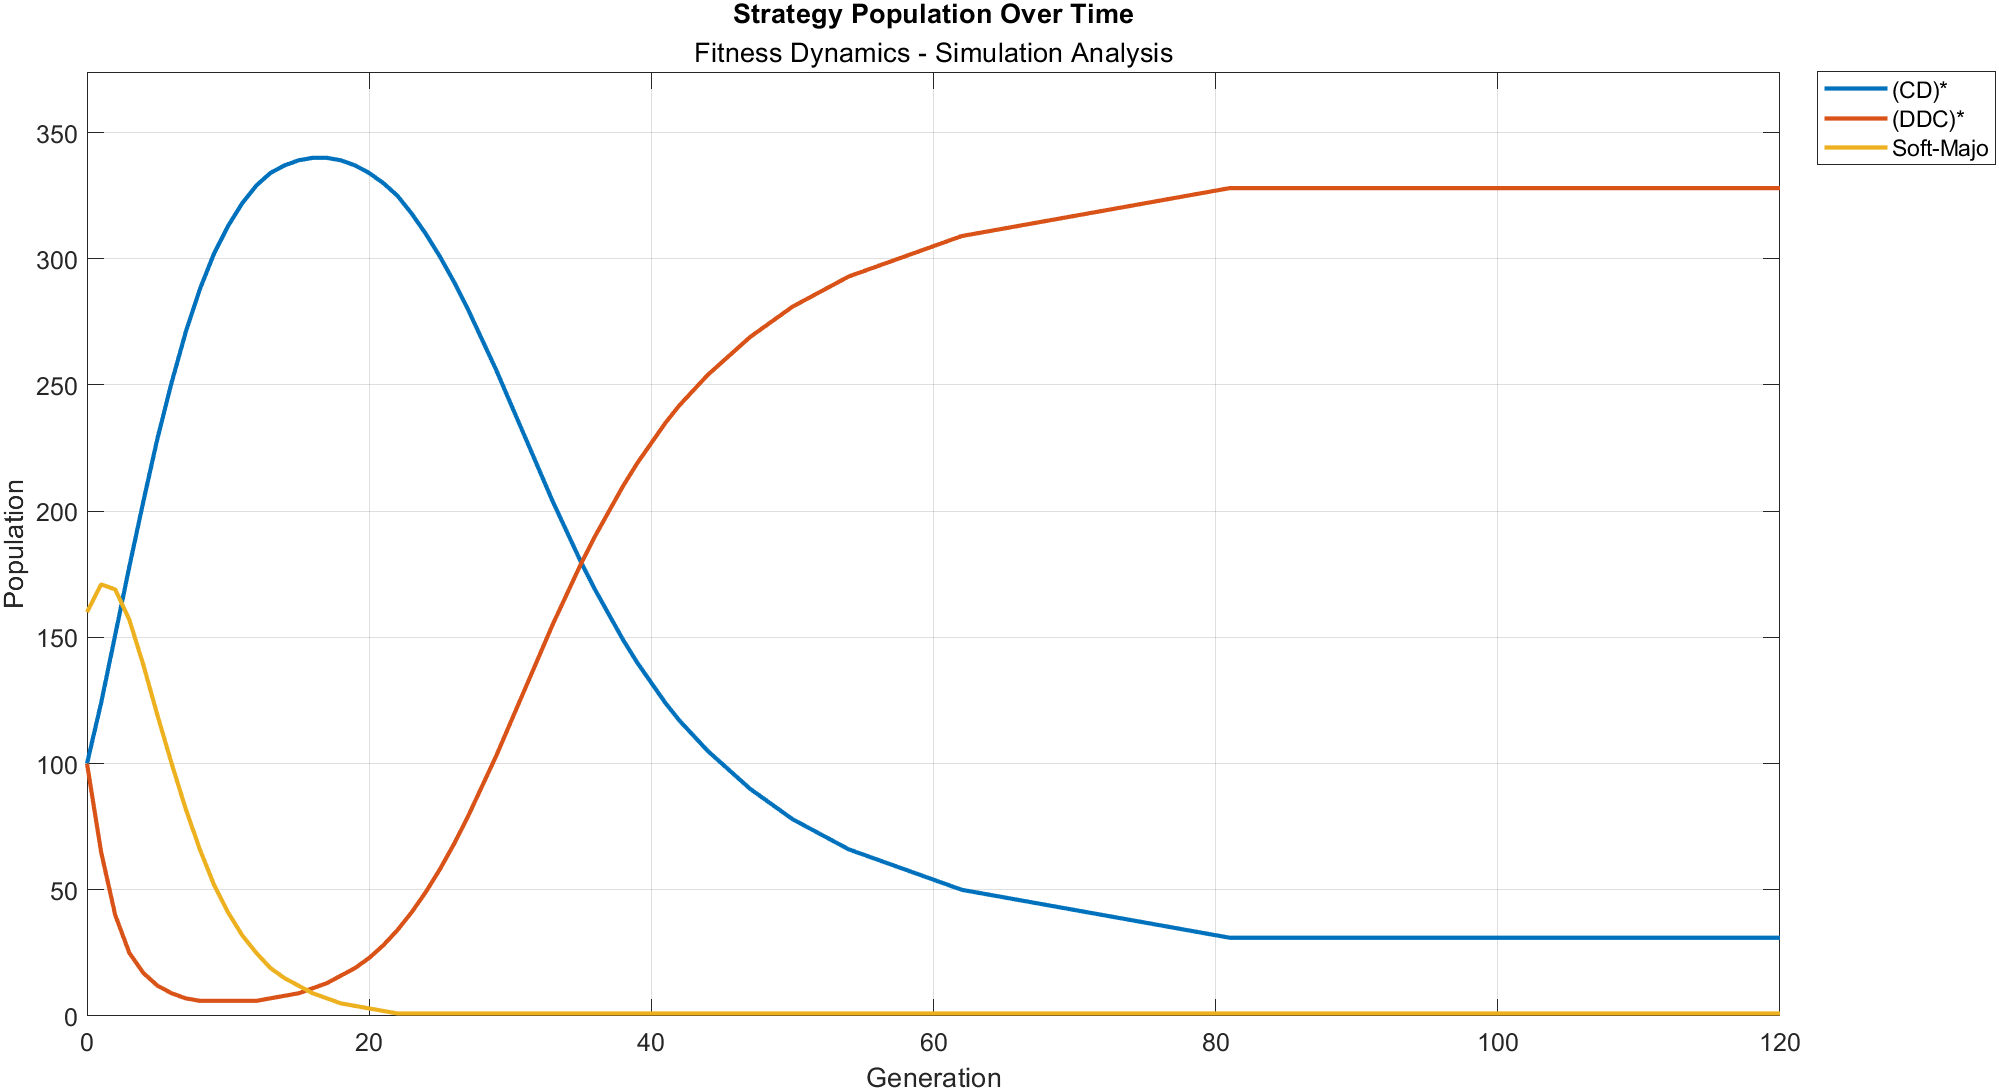
\includegraphics[width=\linewidth]{Figures Fitness Dynamics/example8b-sim.png}
        \caption{Προσομοίωση εξελικτικού πρωταθλήματος}
        \label{fig:fig_fit_8b_c}
        
    \end{subfigure}

    \caption{Αποτελέσματα πειράματος 8β - \foreignlanguage{english}{Script: example8b.m}}
    \label{fig:fig_fit_8b}
\end{figure}

\subsubsection{Ευαισθησία στην διάρκεια του παιχνιδιού}
Για να μελετήσουμε την ευασθησία του πρωταθλήματος στην διάρκεια του παιχνιδιού, πραγματοποιούμε το ίδιο πρωτάθλημα δύο φορές, το πρώτο με 7 κινήσεις συνολικά ενώ το δεύτερο με 6 κινήσεις. Στα Σχήματα \ref{fig:fig_fit_9a} και \ref{fig:fig_fit_9b} παρουσιάζονται τα αποτελέσματα αυτών των πρωταθλημάτων για τις στρατηγικές \foreignlanguage{english}{per\_ccd, per\_ddc} και \foreignlanguage{english}{soft\_majo} με αρχικούς πληθυσμούς 300, 244 και 100 αντίστοιχα.

Παρατηρούμε ότι τα αποτελέσματα των προσομοιώσεων μας και στα δύο πρωταθλήματα είναι παρόμοια με τα αναμενόμενα που παρουσιάζονται στο Σχήμα \ref{fig:fig_fit_9a}. Στα θεωρητικά πρωταθλήματα η ταλάντωση εξασθενεί όσο το πρωτάθλημα εξελίσεται σε αντίθεση με τα πρωταθλήματα των προσομοιώσεων. Συνολικά μπορούμε να διακρίνουμε ότι η διάρκεια 7 κινήσεων συντελεί σε μια περιοδική ταλάντωση ενώ η με 6 κινήσεις η ταλάντωση γίνεται εξασθενημένη.

\begin{figure}[htbp]
    \centering

    \begin{subfigure}[b]{0.5\linewidth}
        \centering
        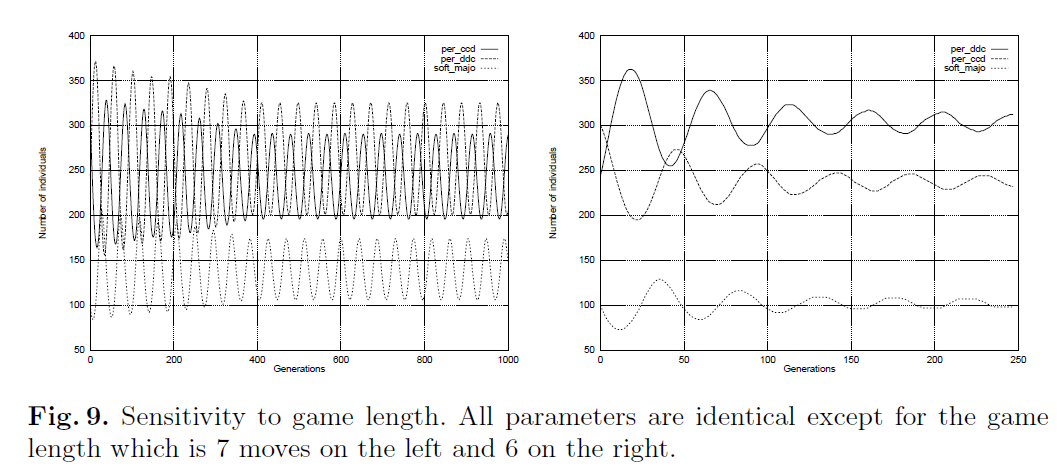
\includegraphics[width=\linewidth]{Figures Fitness Dynamics/9.png}
        \caption{Θεωρητικό αποτέλεσμα από προηγούμενη δημοσίευση. \textit{Πηγή:} \protect\cite{mathieu1999}}
        \label{fig:fig_fit_9_a}
    \end{subfigure}
    \hfill
    \begin{subfigure}[b]{0.5\linewidth}
        \centering
        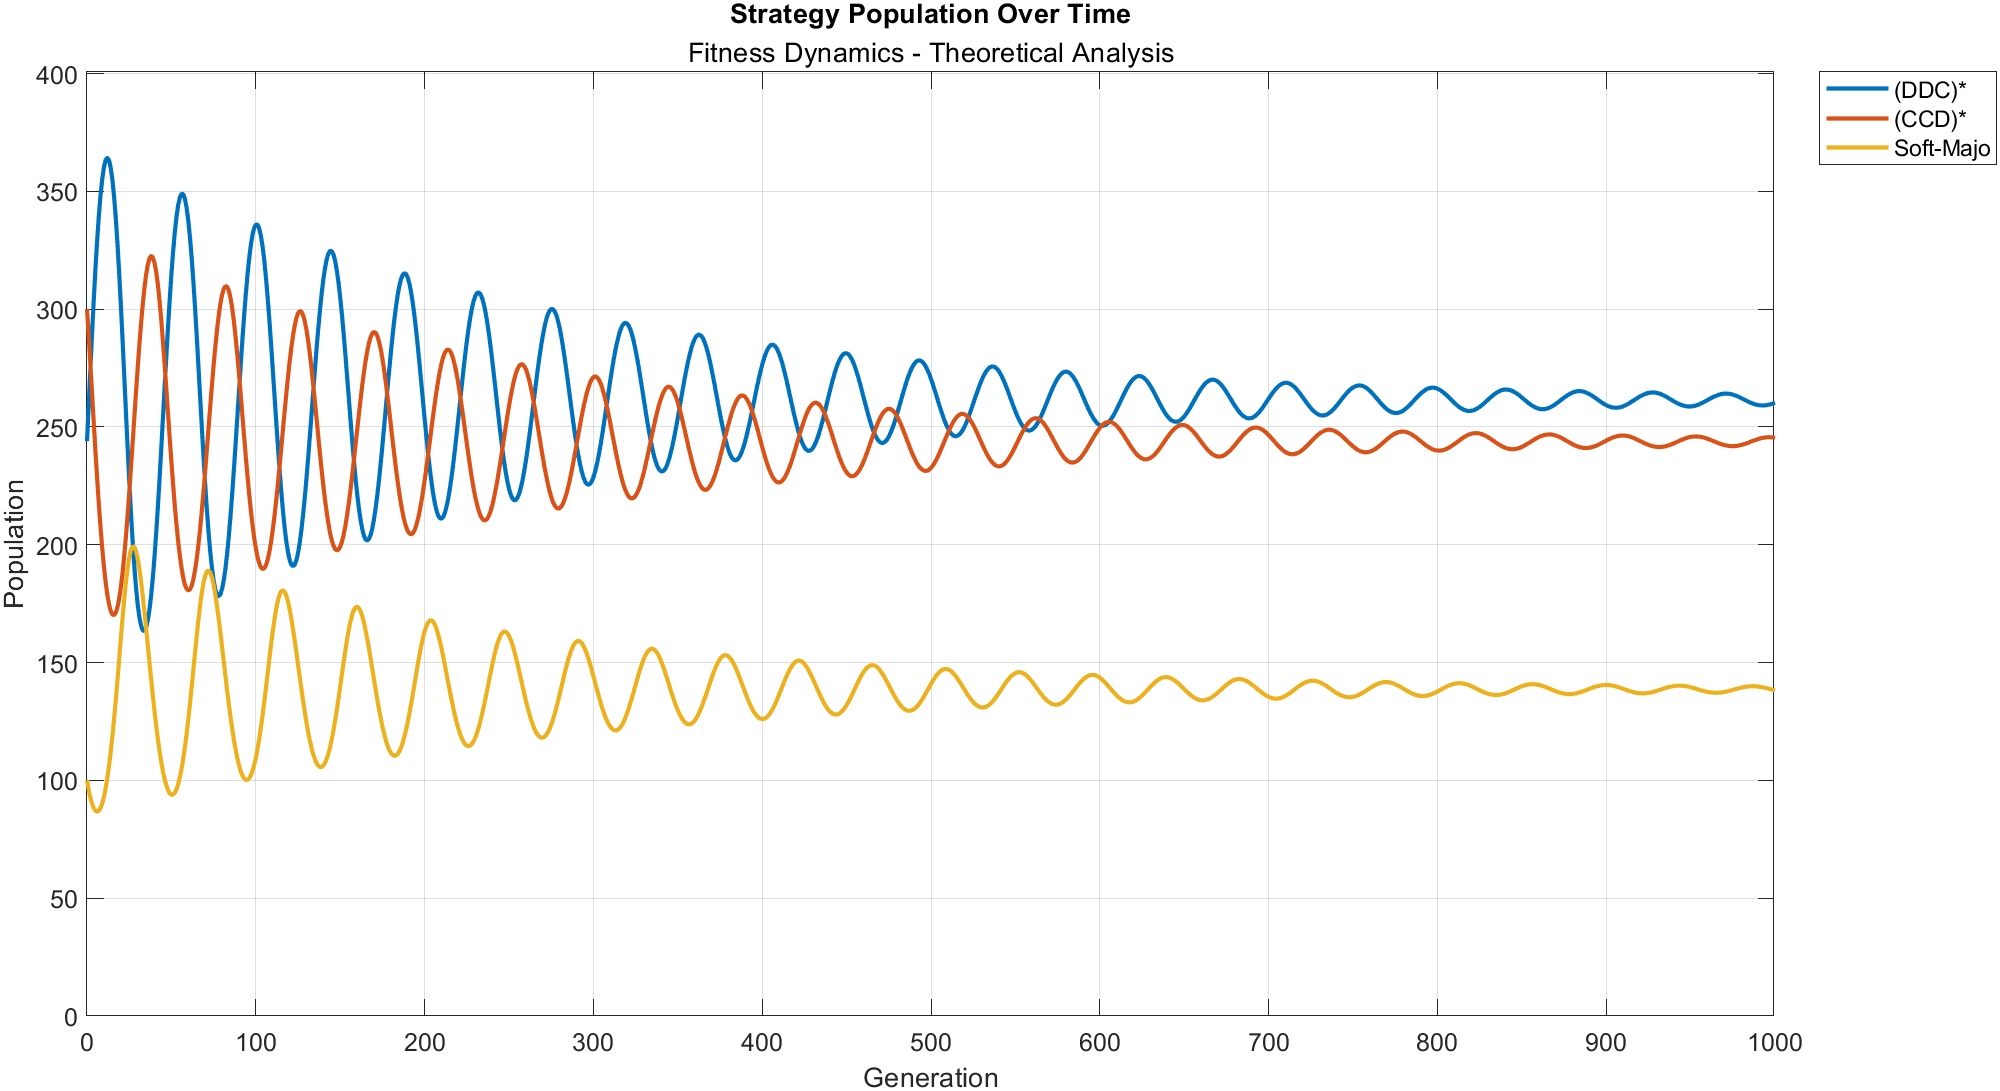
\includegraphics[width=\linewidth]{Figures Fitness Dynamics/example9a.png}
        \caption{Θεωρητικό εξελικτικό πρωτάθλημα}
        \label{fig:fig_fit_9a_b}
    \end{subfigure}
    \hfill
    \begin{subfigure}[b]{0.5\linewidth}
        \centering
        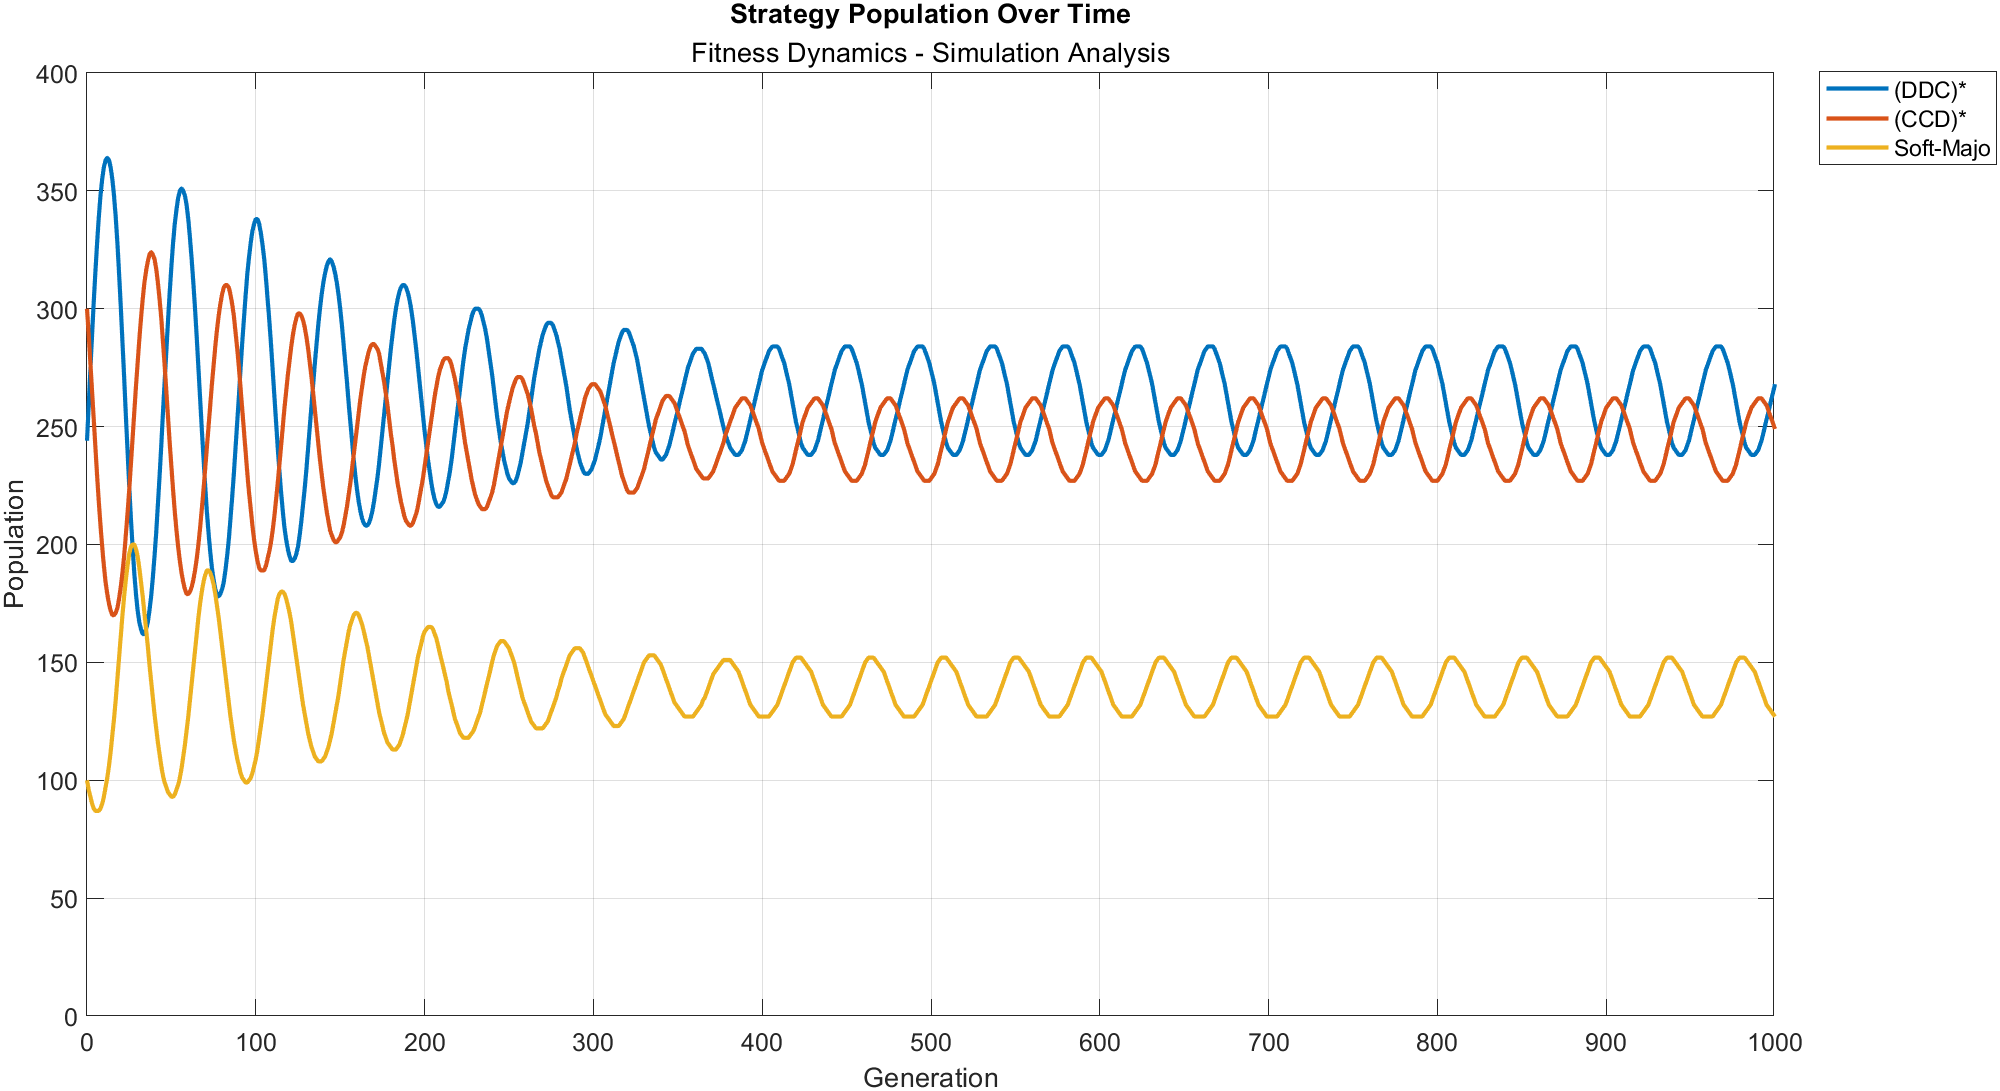
\includegraphics[width=\linewidth]{Figures Fitness Dynamics/example9a-sim.png}
        \caption{Προσομοίωση εξελικτικού πρωταθλήματος}
        \label{fig:fig_fit_9a_c}
        
    \end{subfigure}

    \caption{Αποτελέσματα πειράματος 9α - \foreignlanguage{english}{Script: example9a.m}}
    \label{fig:fig_fit_9a}
\end{figure}

\begin{figure}[htbp]
    \centering

    \begin{subfigure}[b]{0.5\linewidth}
        \centering
        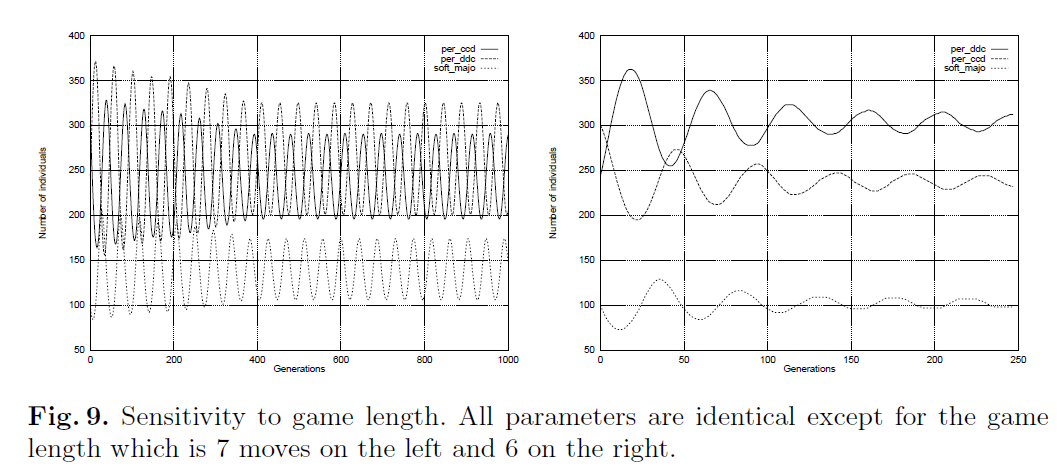
\includegraphics[width=\linewidth]{Figures Fitness Dynamics/9.png}
        \caption{Θεωρητικό αποτέλεσμα από προηγούμενη δημοσίευση. \textit{Πηγή:} \protect\cite{mathieu1999}}
    \end{subfigure}
    \hfill
    \begin{subfigure}[b]{0.5\linewidth}
        \centering
        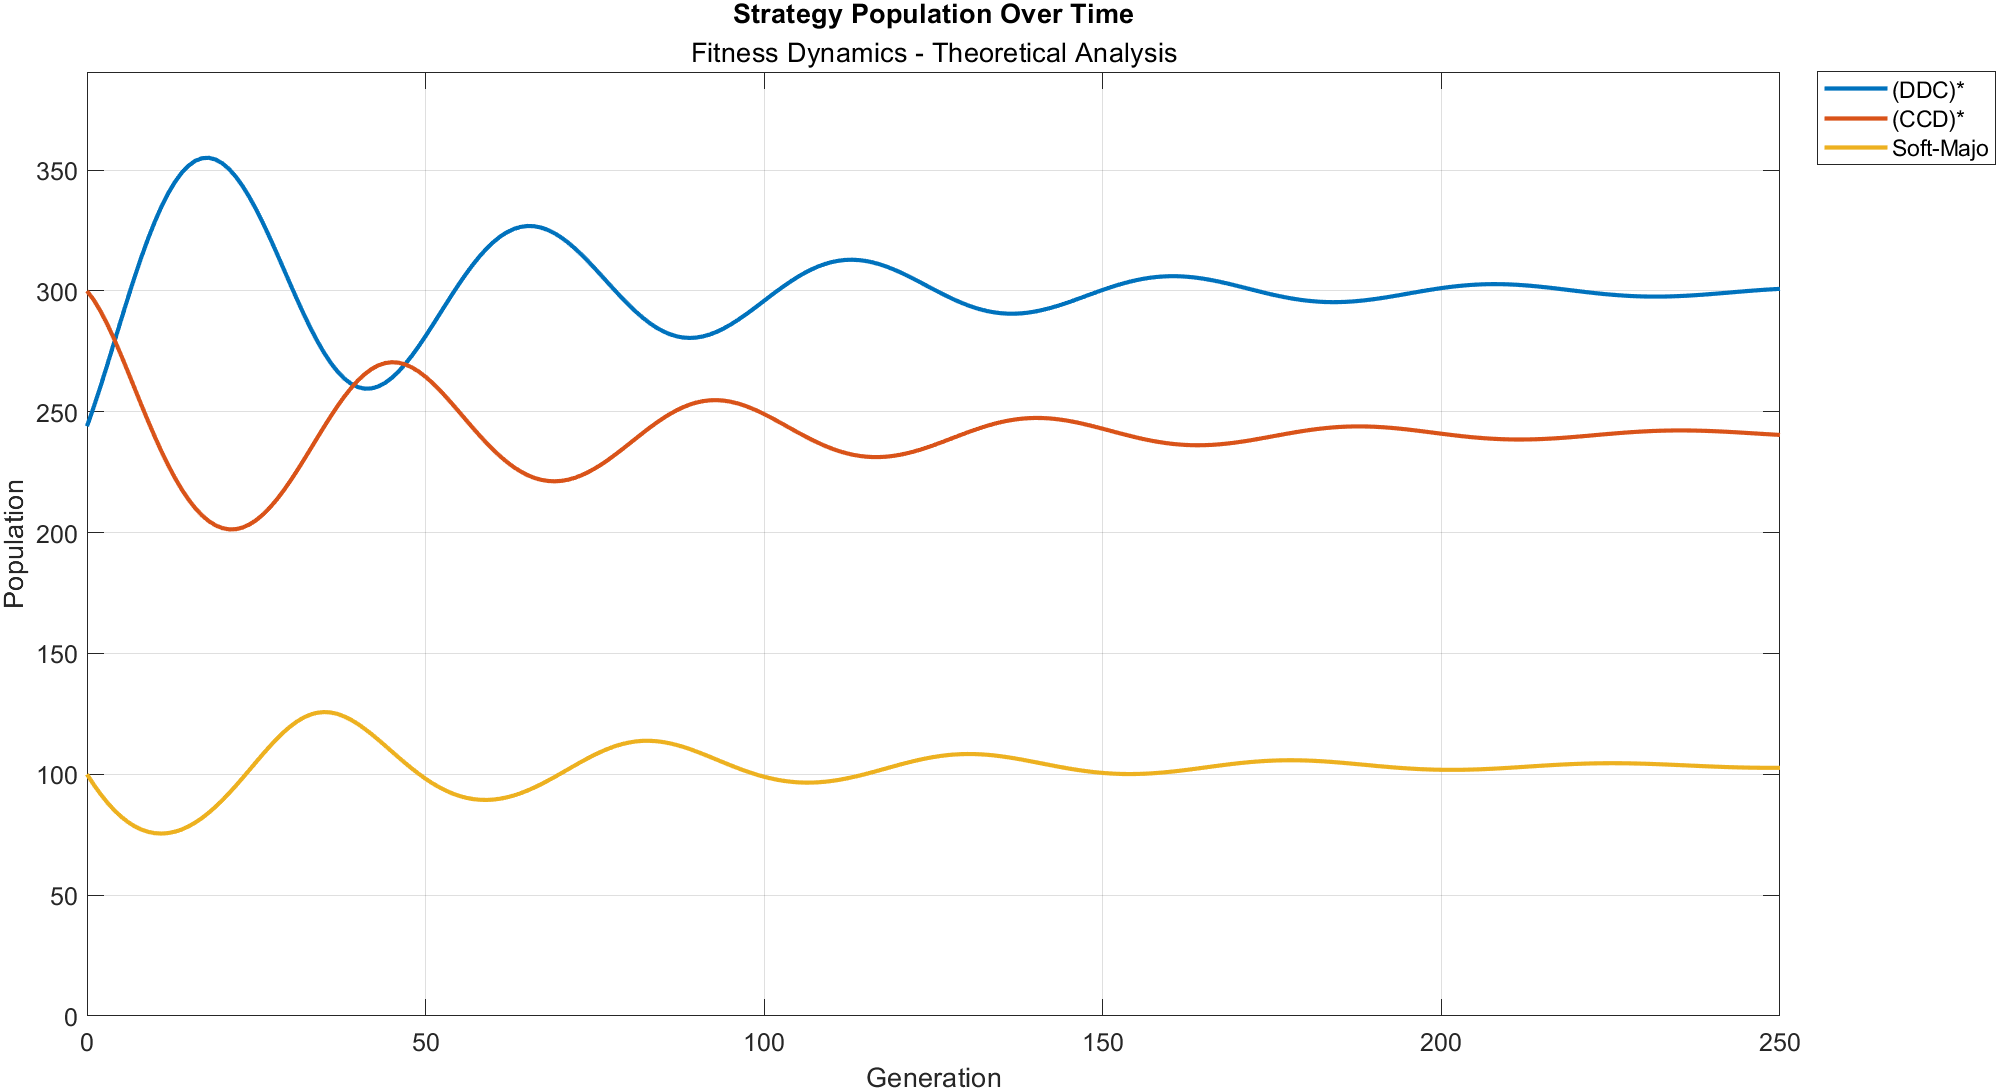
\includegraphics[width=\linewidth]{Figures Fitness Dynamics/example9b.png}
        \caption{Θεωρητικό εξελικτικό πρωτάθλημα}
        \label{fig:fig_fit_9b_b}
    \end{subfigure}
    \hfill
    \begin{subfigure}[b]{0.5\linewidth}
        \centering
        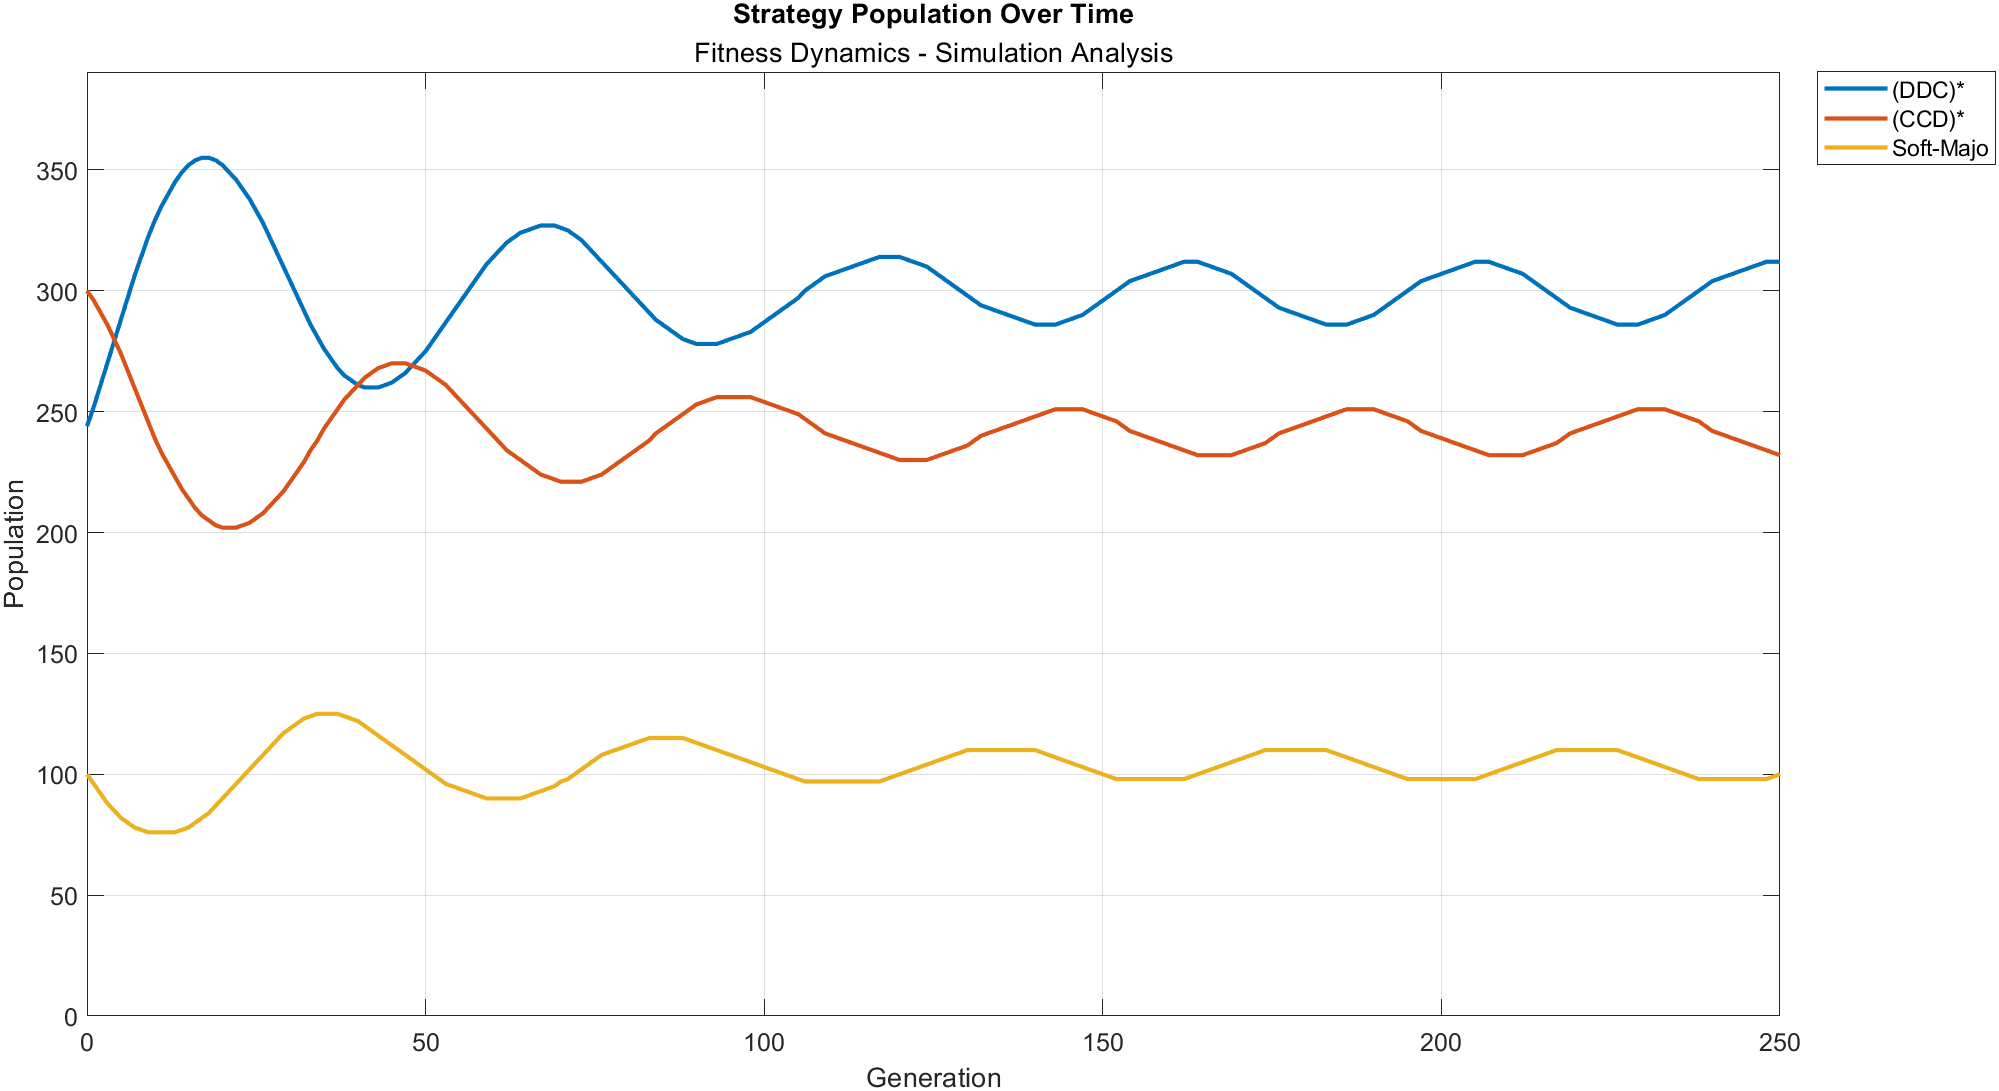
\includegraphics[width=\linewidth]{Figures Fitness Dynamics/example9b-sim.png}
        \caption{Προσομοίωση εξελικτικού πρωταθλήματος}
        \label{fig:fig_fit_9b_c}
        
    \end{subfigure}

    \caption{Αποτελέσματα πειράματος 9β - \foreignlanguage{english}{Script: example9b.m}}
    \label{fig:fig_fit_9b}
\end{figure}

\subsubsection{Ευαισθησία στην απόδοση \foreignlanguage{english}{CIPD} }
Για να μελετήσουμε την επίδραση των παραμέτρων του πίνακα απολαβών στο Δίλημμα του Φυλακισμένου ως προς την εξέλιξη του πρωταθλήματος, διεξάγουμε δύο τουρνουά: το πρώτο με τιμή παραμέτρου $T = 4{,}6$ και το δεύτερο με $T = 4{,}7$. Στα Σχήματα \ref{fig:fig_fit_10a} και \ref{fig:fig_fit_10b} παρουσιάζονται τα αποτελέσματα των προσομοιώσεων για τις στρατηγικές \foreignlanguage{english}{per\_ccd}, \foreignlanguage{english}{per\_ddc} και \foreignlanguage{english}{soft\_majo}, με αρχικούς πληθυσμούς 300, 244 και 100 αντίστοιχα.


Παρατηρούμε ότι τα αποτελέσματα των προσομοιώσεων μας και στις δυο περιπτώσεις συμπίπτουν πλήρως με τα αναμενόμενα. Επομένως στο πρώτο πρωτάθλημα παρατηρείται μια αυξανόμενη ταλάντωση ενώ στο δεύτερο η κίνηση γίνεται περιοδική.

\begin{figure}[htbp]
    \centering

    \begin{subfigure}[b]{0.5\linewidth}
        \centering
        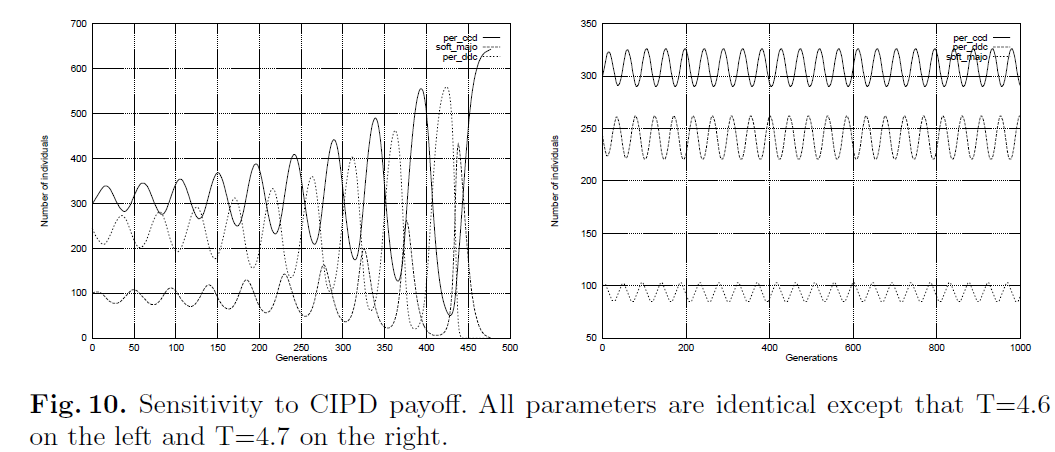
\includegraphics[width=\linewidth]{Figures Fitness Dynamics/10.png}
        \caption{Θεωρητικό αποτέλεσμα από προηγούμενη δημοσίευση. \textit{Πηγή:} \protect\cite{mathieu1999}}
        \label{fig:fig_fit_10_a}
    \end{subfigure}
    \hfill
    \begin{subfigure}[b]{0.5\linewidth}
        \centering
        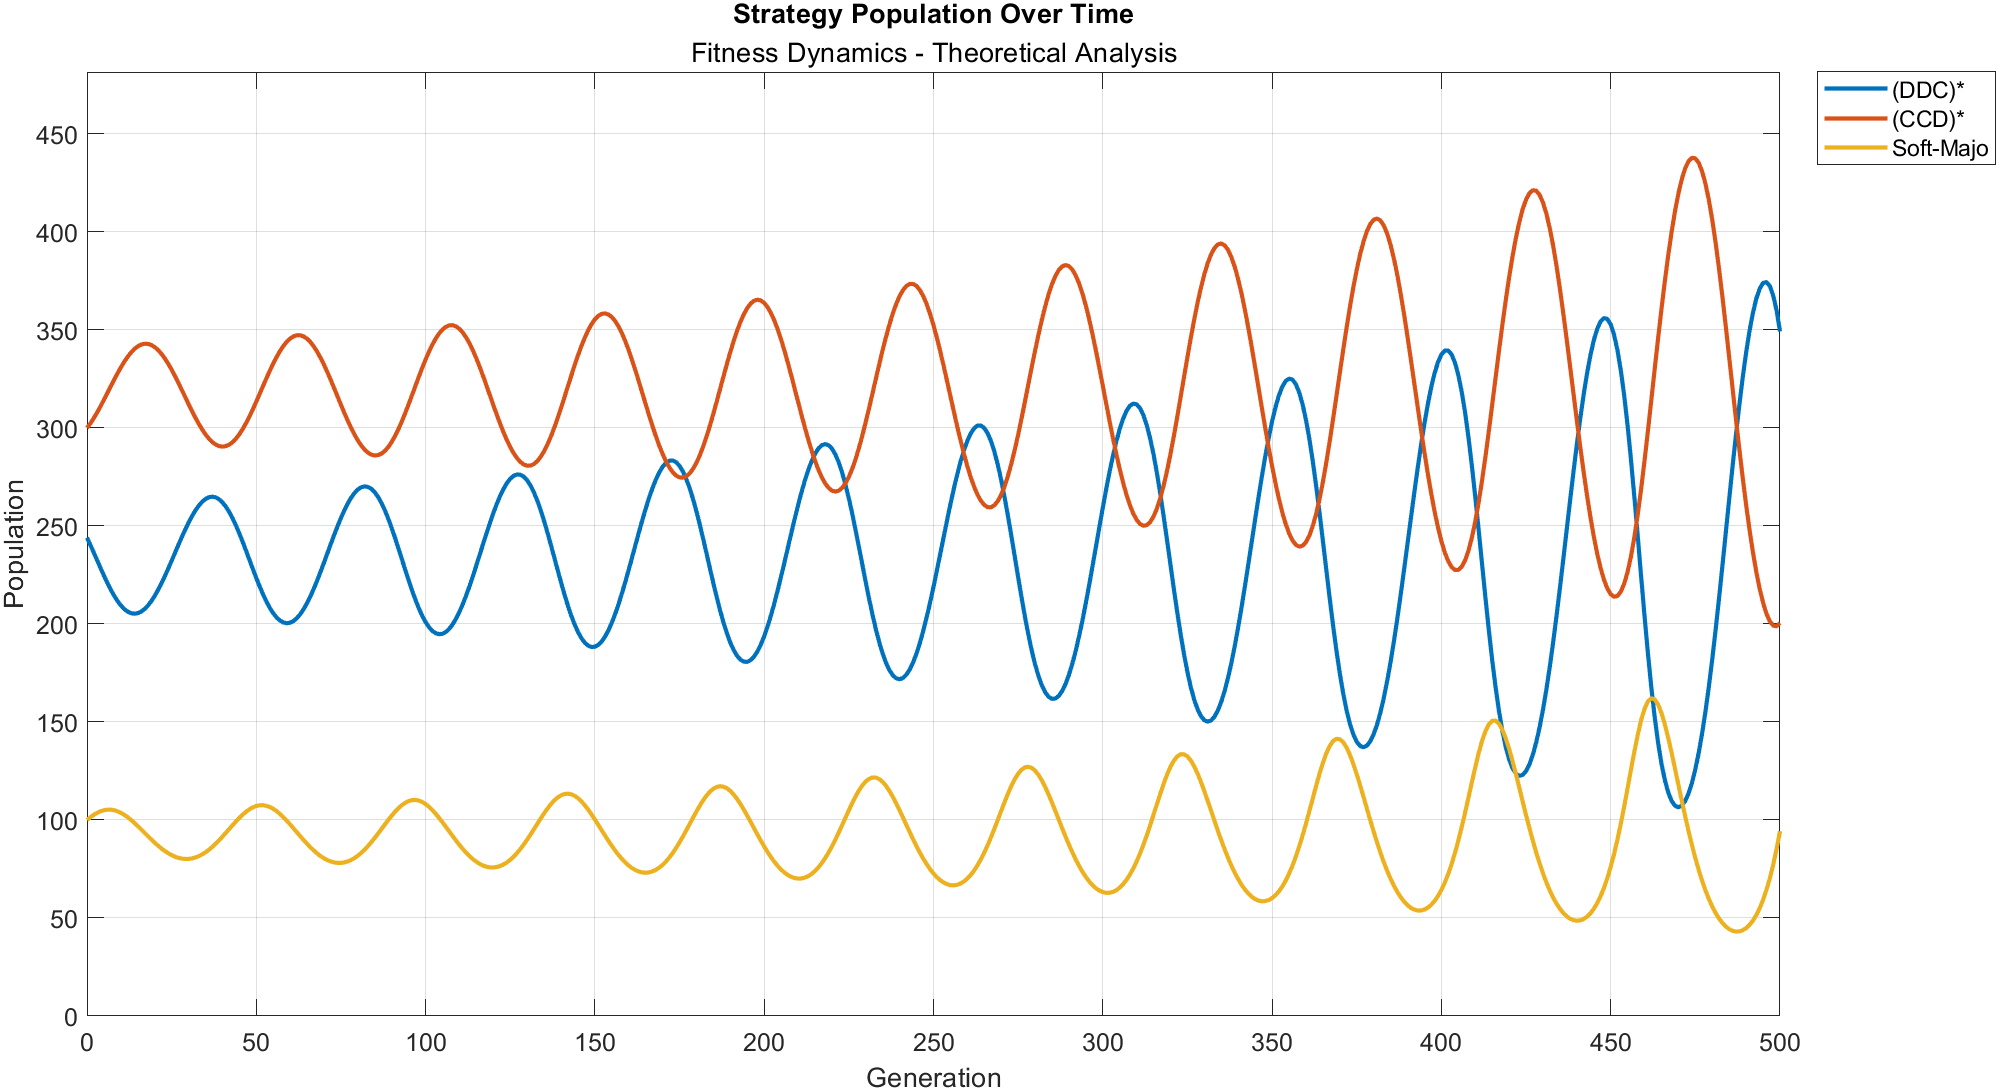
\includegraphics[width=\linewidth]{Figures Fitness Dynamics/example10a.png}
        \caption{Θεωρητικό εξελικτικό πρωτάθλημα}
        \label{fig:fig_fit_10a_b}
    \end{subfigure}
    \hfill
    \begin{subfigure}[b]{0.5\linewidth}
        \centering
        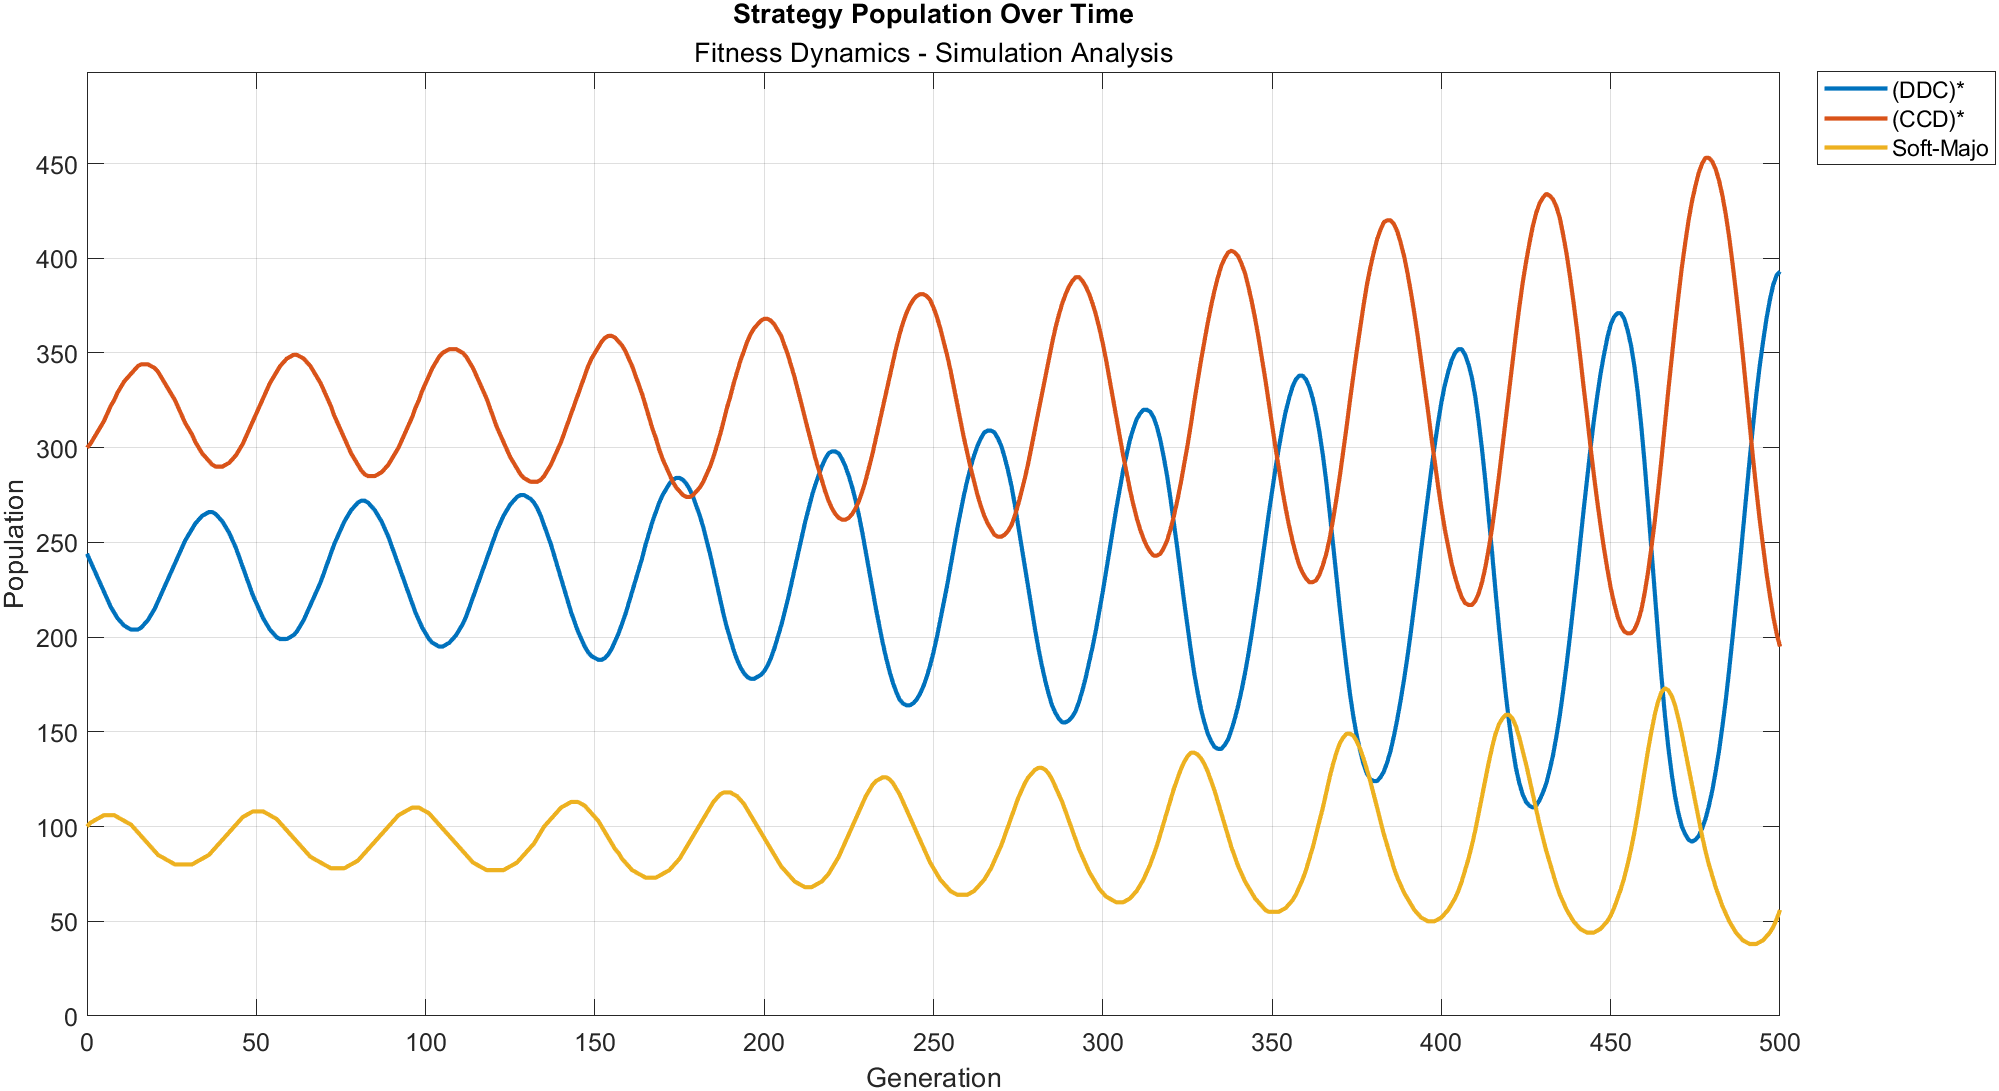
\includegraphics[width=\linewidth]{Figures Fitness Dynamics/example10a-sim.png}
        \caption{Προσομοίωση εξελικτικού πρωταθλήματος}
        \label{fig:fig_fit_10a_c}
        
    \end{subfigure}

    \caption{Αποτελέσματα πειράματος 10α - \foreignlanguage{english}{Script: example10a.m}}
    \label{fig:fig_fit_10a}
\end{figure}

\begin{figure}[htbp]
    \centering

    \begin{subfigure}[b]{0.5\linewidth}
        \centering
        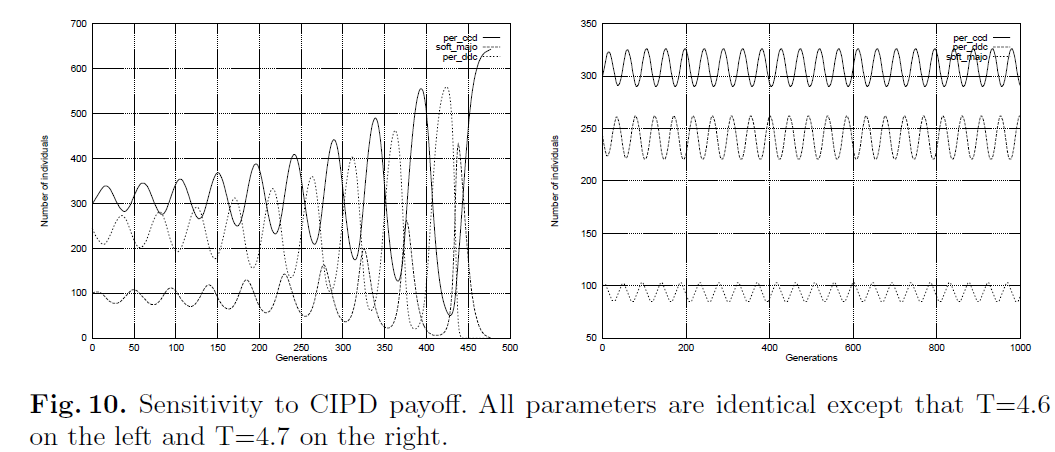
\includegraphics[width=\linewidth]{Figures Fitness Dynamics/10.png}
        \caption{Θεωρητικό αποτέλεσμα από προηγούμενη δημοσίευση. \textit{Πηγή:} \protect\cite{mathieu1999}}
    \end{subfigure}
    \hfill
    \begin{subfigure}[b]{0.5\linewidth}
        \centering
        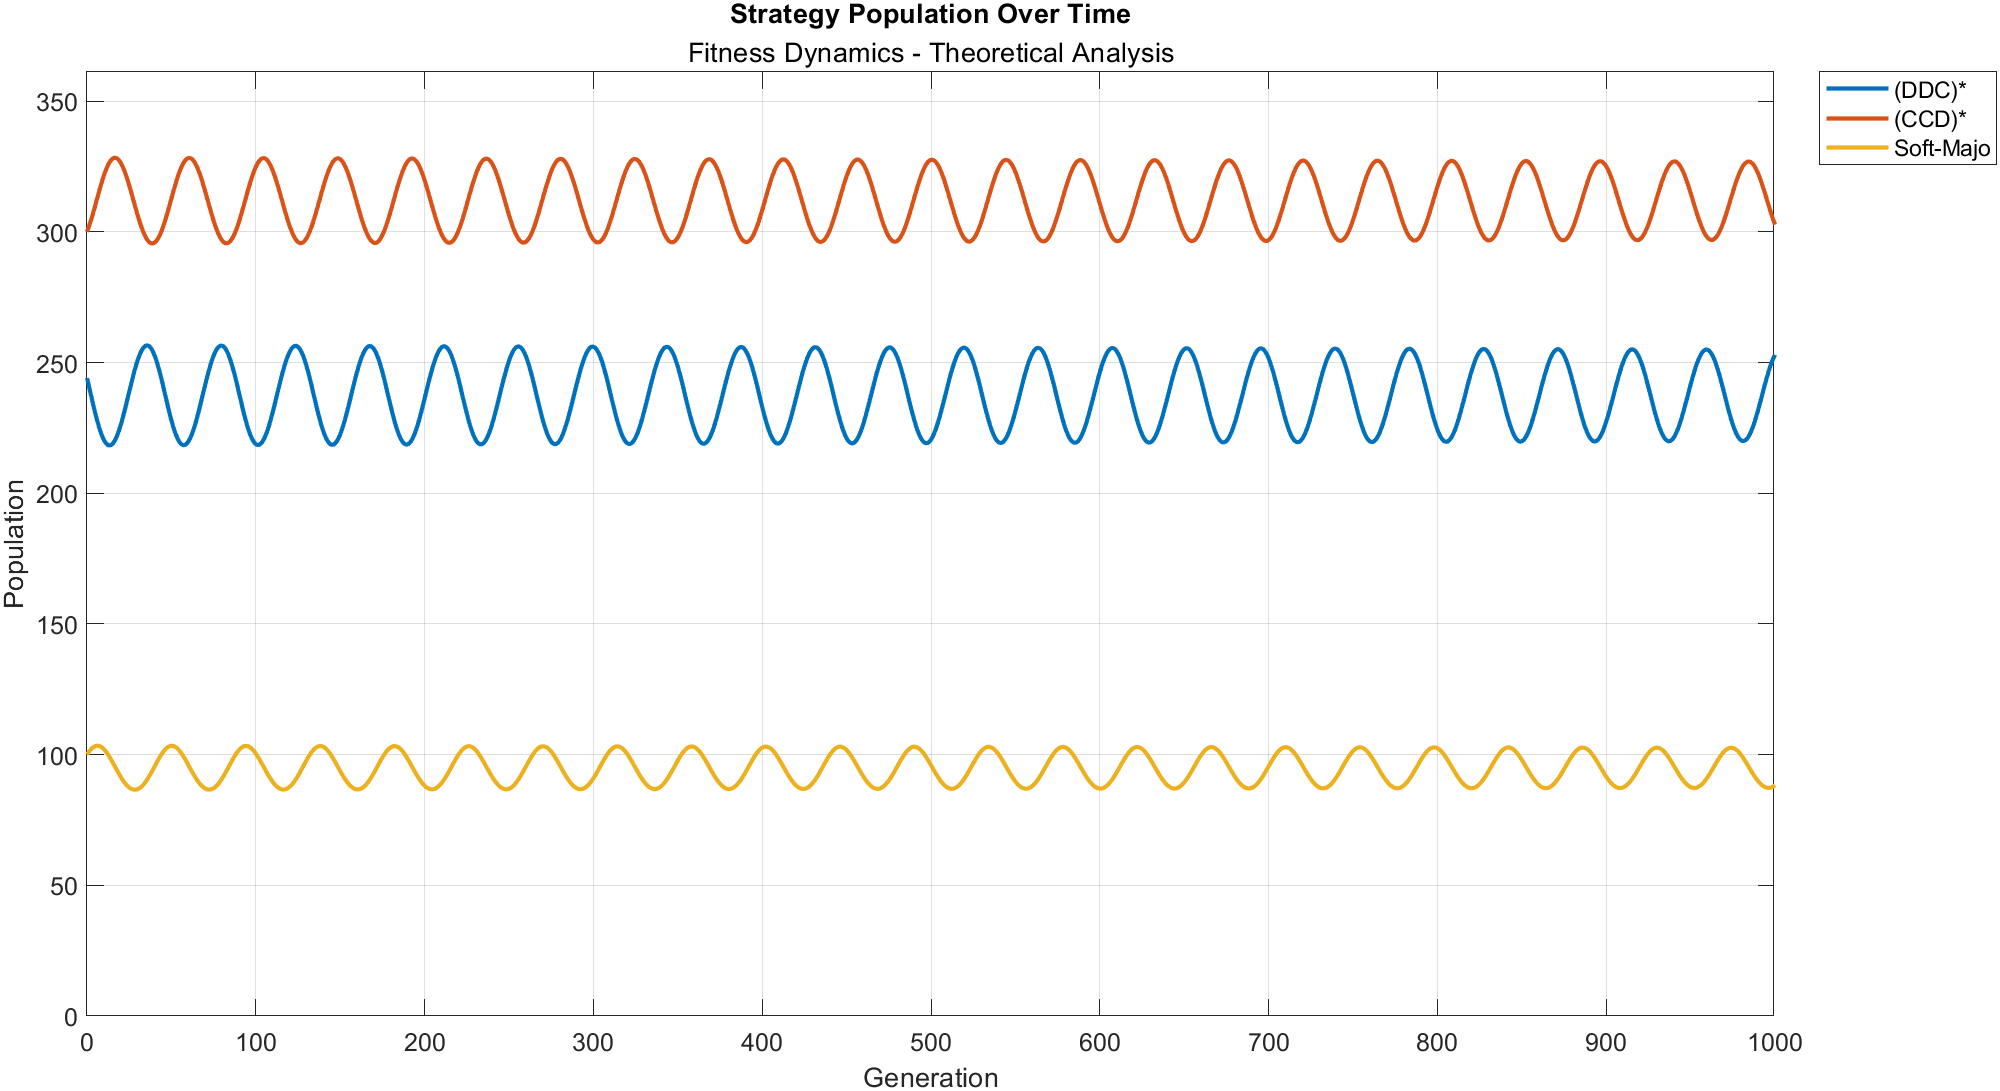
\includegraphics[width=\linewidth]{Figures Fitness Dynamics/example10b.png}
        \caption{Θεωρητικό εξελικτικό πρωτάθλημα}
        \label{fig:fig_fit_10b_b}
    \end{subfigure}
    \hfill
    \begin{subfigure}[b]{0.5\linewidth}
        \centering
        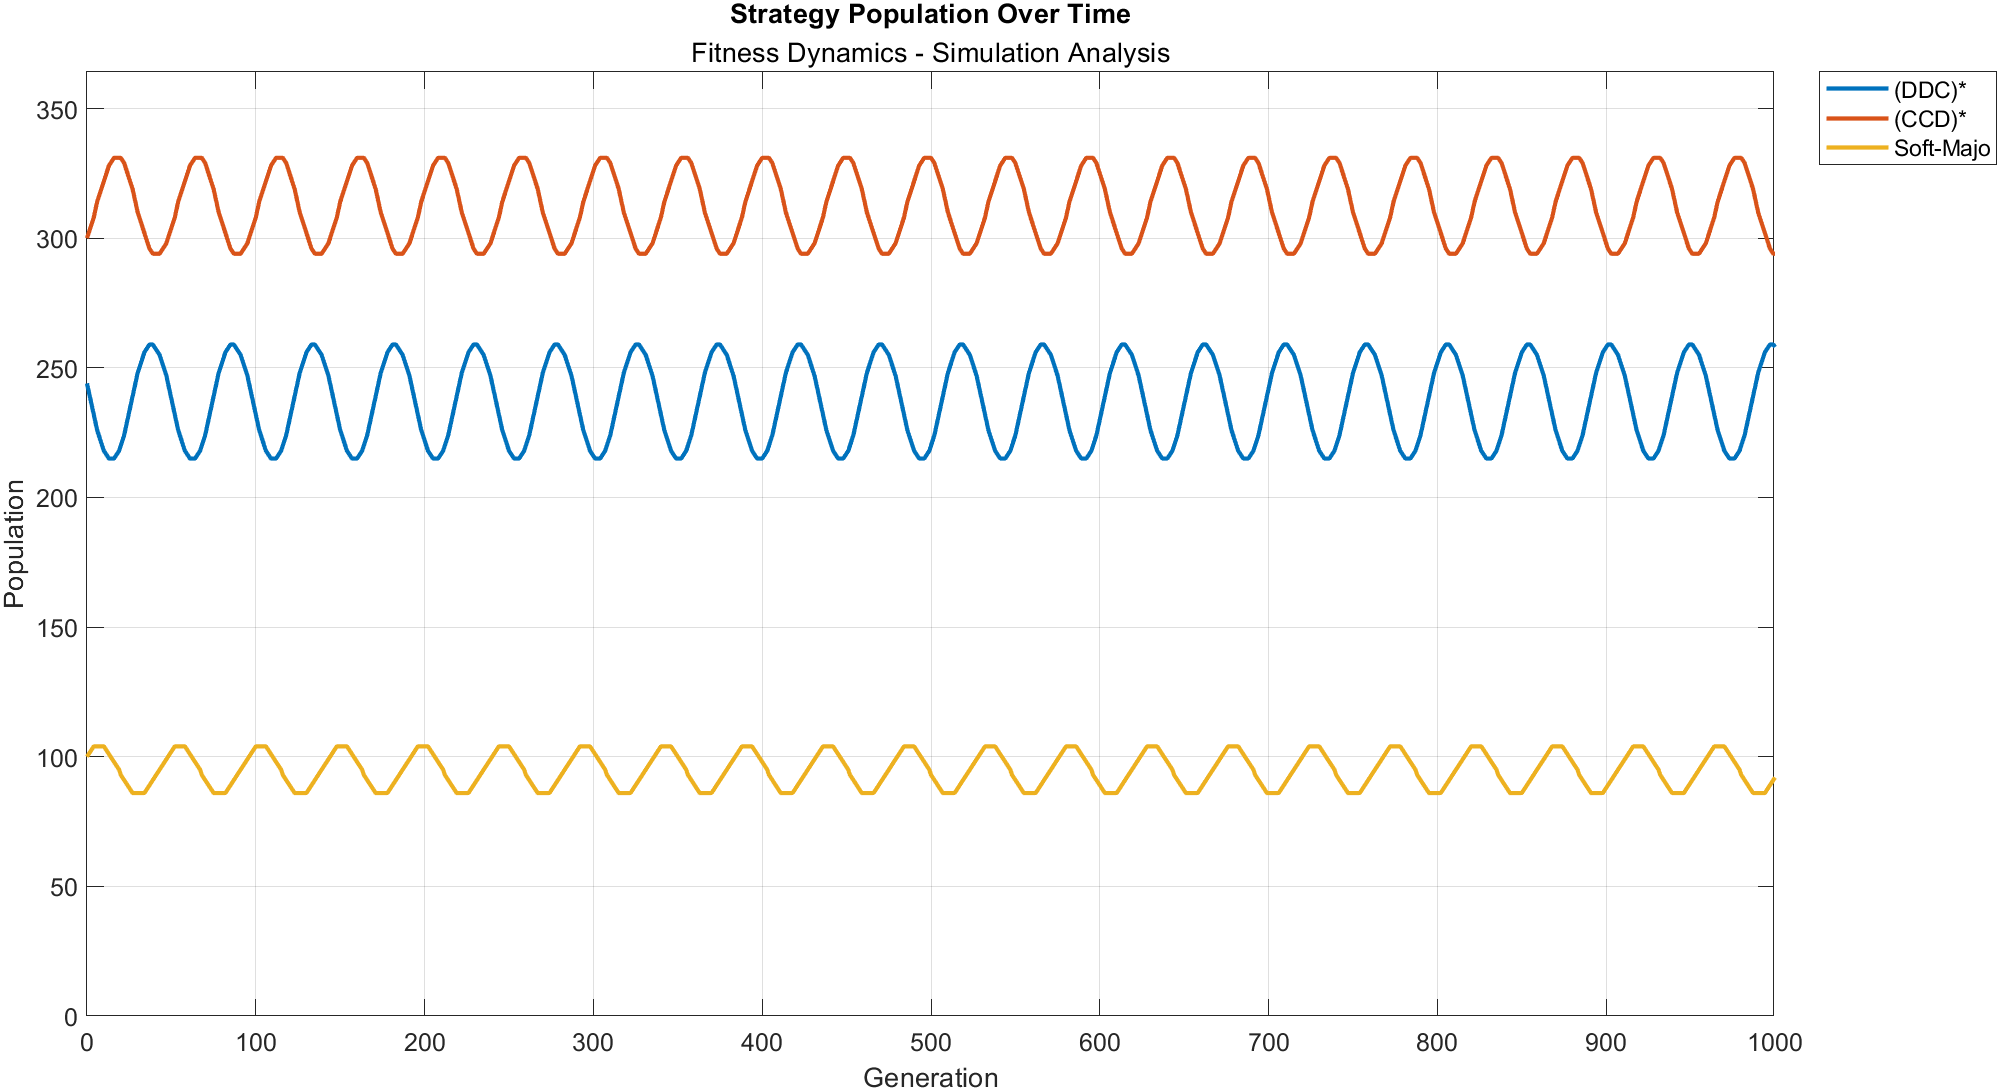
\includegraphics[width=\linewidth]{Figures Fitness Dynamics/example10b-sim.png}
        \caption{Προσομοίωση εξελικτικού πρωταθλήματος}
        \label{fig:fig_fit_10b_c}
        
    \end{subfigure}

    \caption{Αποτελέσματα πειράματος 10β - \foreignlanguage{english}{Script: example10b.m}}
    \label{fig:fig_fit_10b}
\end{figure}

\subsubsection{Ευαισθησία στη μέθοδο ανακατανομής του πληθυσμού}
Για να μελετηθεί η επίδραση της μεθόδου ανακατανομής του πληθυσμού στην εξέλιξη του πρωταθλήματος, διεξάγονται τα εξής δύο πειράματα.

\subsubsection*{Πρώτο πείραμα}
Στο πρώτο πείραμα συγκρίνουμε την μεθόδο της στρογγυλοποίησης με την χρήση δεκαδικών παικτών για την ανακατανομή του πληθυσμού.
Στα Σχήματα \ref{fig:fig_fit_11a} και \ref{fig:fig_fit_11b} παρουσιάζονται τα αποτελέσματα αυτών των πρωταθλημάτων για τις στρατηγικές \foreignlanguage{english}{per\_ccd}, \foreignlanguage{english}{per\_ddc} και \foreignlanguage{english}{soft\_majo}, με αρχικούς πληθυσμούς 300, 200 και 100 αντίστοιχα.

Η θεωρητική ανάλυση προβλέπει ότι η στρογγυλοποίηση οδηγεί σε περιοδική ταλάντωση, ενώ η χρήση δεκαδικών παικτών παράγει φθίνουσα (αποσβεννυμένη) ταλάντωση.
Στο πρώτο πρωτάθλημα όλα τα αποτελέσματα συμφωνούν με τα προβλεπόμενα, καθώς παρατηρείται μια φθίνουσα ταλάντωση.
Στο δεύτερο πρωτάθλημα, και οι δύο προσομοιώσεις εμφανίζουν φθίνουσες ταλαντώσεις, σε αντίθεση με το αναμενόμενο αποτέλεσμα της θεωρητικής ανάλυσης, η οποία προέβλεπε ενίσχυση των διακυμάνσεων.

\begin{figure}[htbp]
    \centering

    \begin{subfigure}[b]{0.5\linewidth}
        \centering
        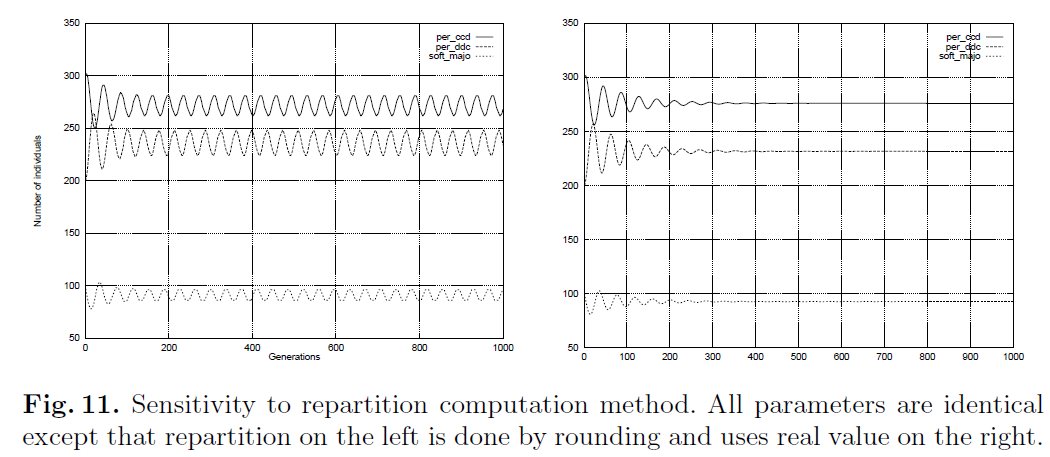
\includegraphics[width=\linewidth]{Figures Fitness Dynamics/11.png}
        \caption{Θεωρητικό αποτέλεσμα από προηγούμενη δημοσίευση. \textit{Πηγή:} \protect\cite{mathieu1999}}
        \label{fig:fig_fit_11_a}
    \end{subfigure}
    \hfill
    \begin{subfigure}[b]{0.5\linewidth}
        \centering
        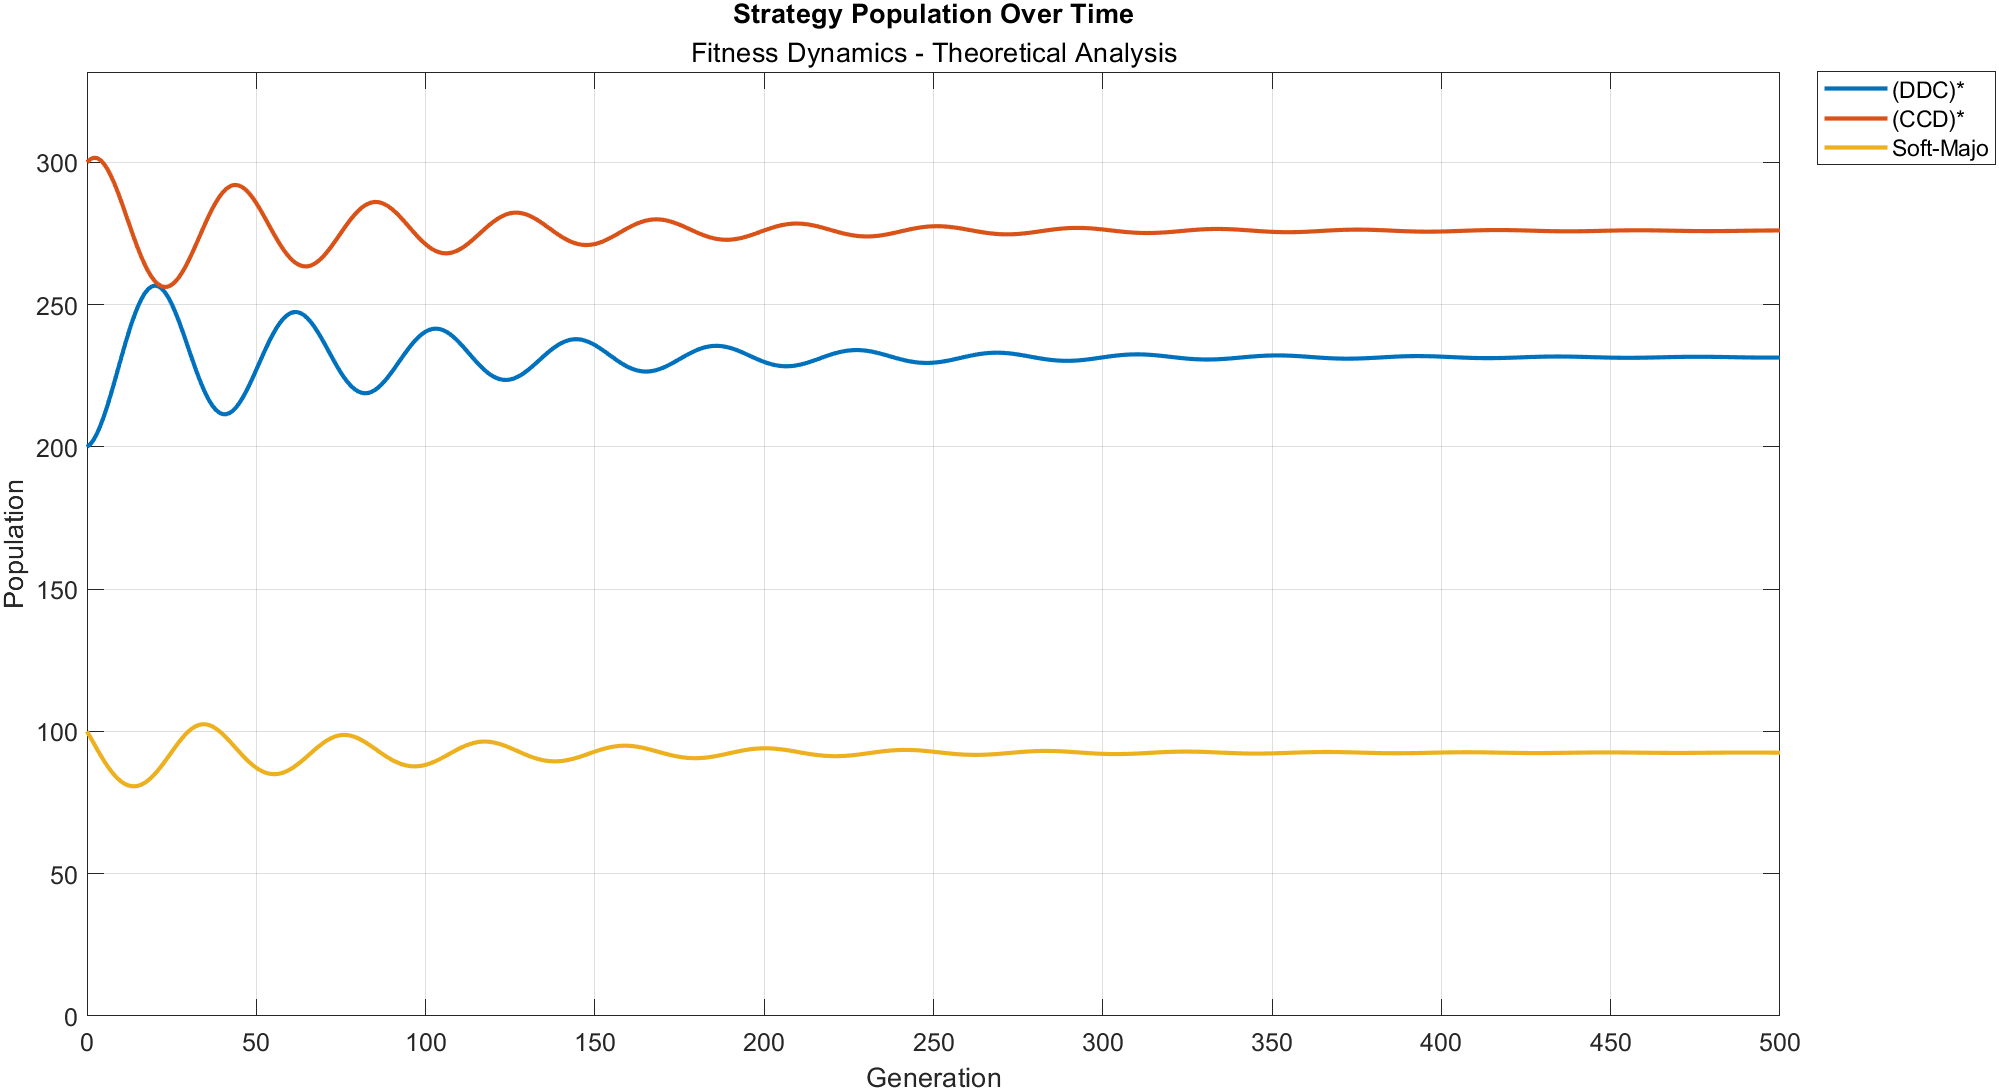
\includegraphics[width=\linewidth]{Figures Fitness Dynamics/example11a.png}
        \caption{Θεωρητικό εξελικτικό πρωτάθλημα}
        \label{fig:fig_fit_11a_b}
    \end{subfigure}
    \hfill
    \begin{subfigure}[b]{0.5\linewidth}
        \centering
        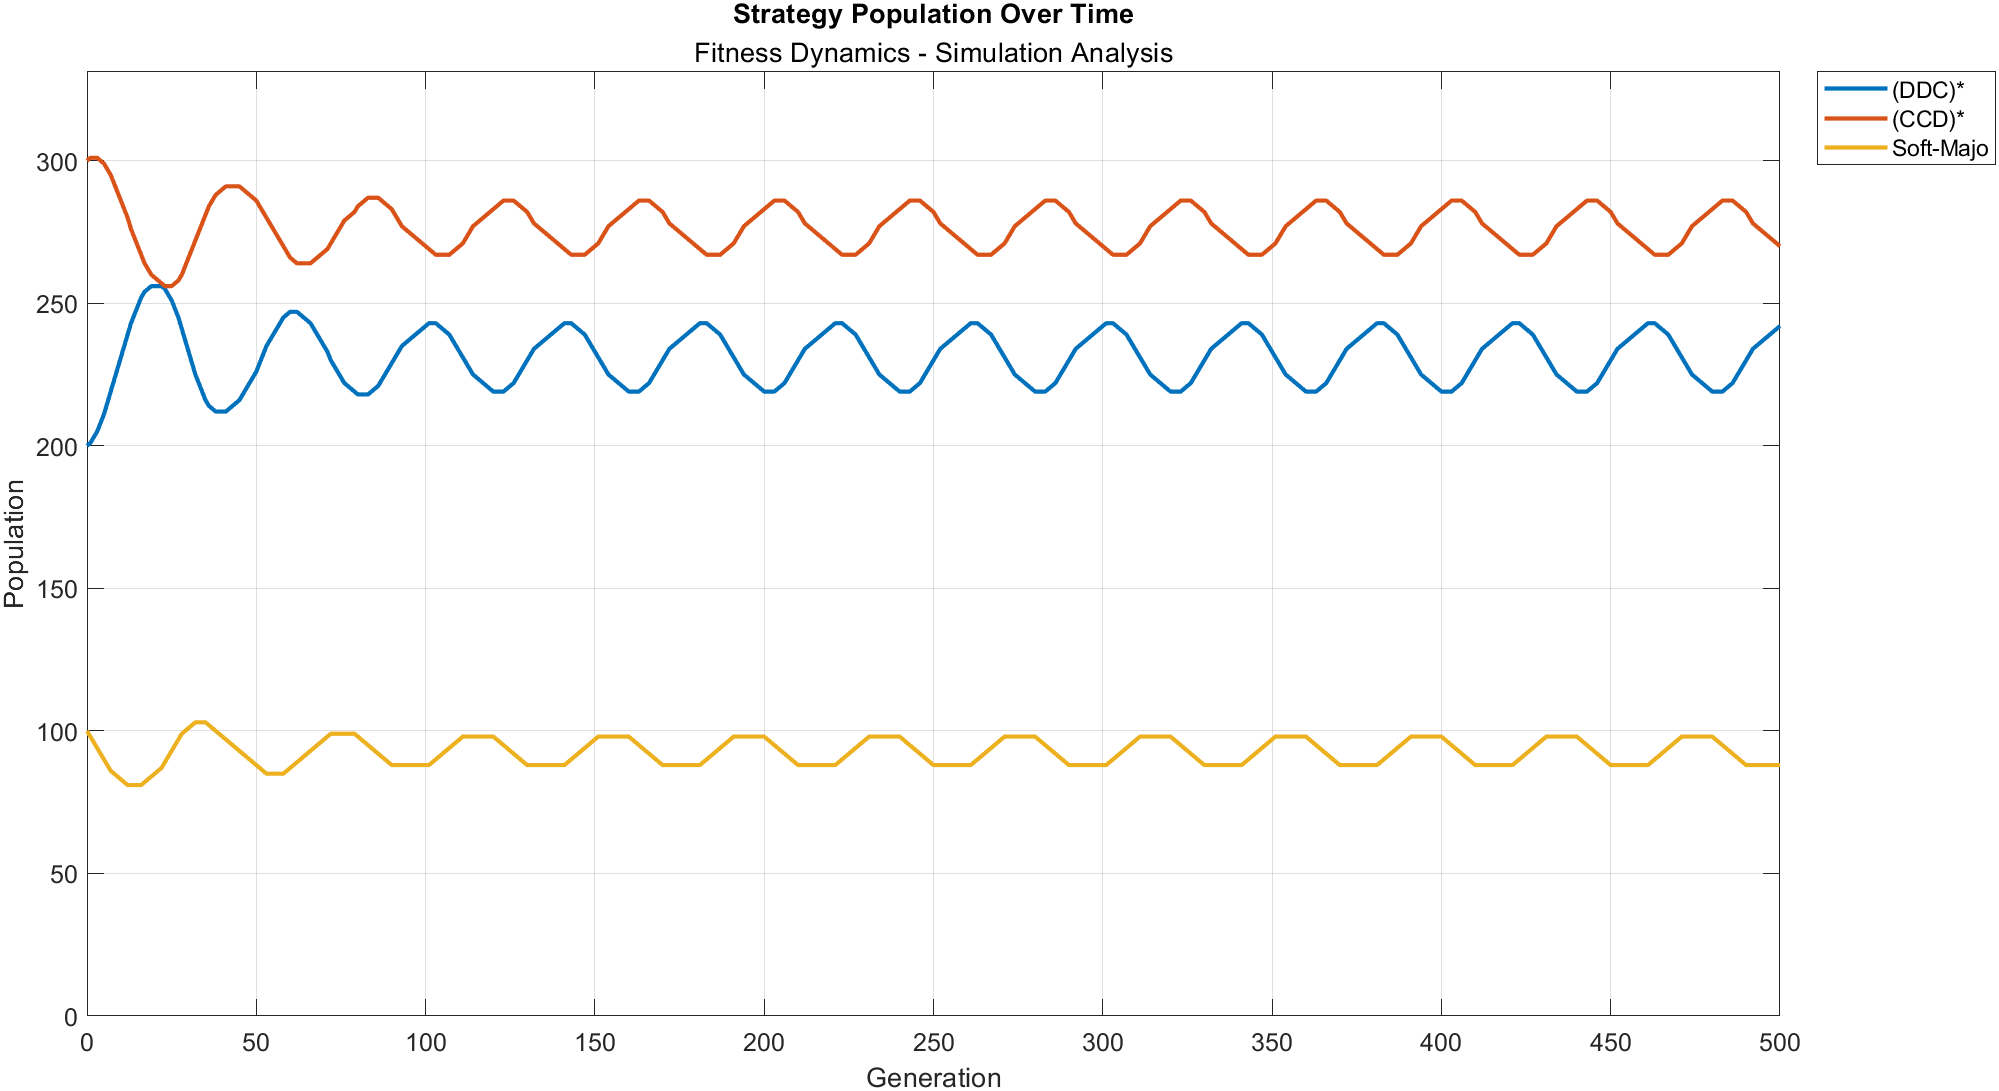
\includegraphics[width=\linewidth]{Figures Fitness Dynamics/example11a-sim.png}
        \caption{Προσομοίωση εξελικτικού πρωταθλήματος}
        \label{fig:fig_fit_11a_c}
        
    \end{subfigure}

    \caption{Αποτελέσματα πειράματος 11α - \foreignlanguage{english}{Script: example11a.m}}
    \label{fig:fig_fit_11a}
\end{figure}

\begin{figure}[htbp]
    \centering

    \begin{subfigure}[b]{0.5\linewidth}
        \centering
        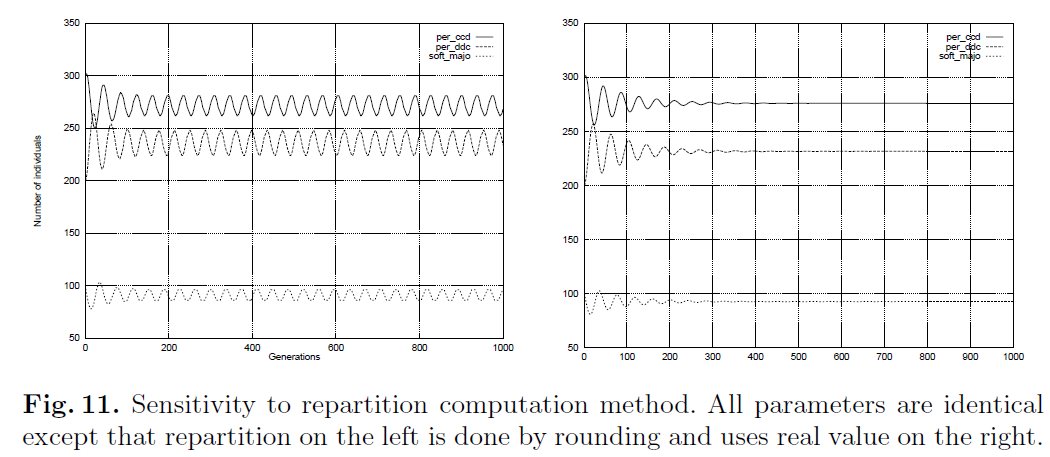
\includegraphics[width=\linewidth]{Figures Fitness Dynamics/11.png}
        \caption{Θεωρητικό αποτέλεσμα από προηγούμενη δημοσίευση. \textit{Πηγή:} \protect\cite{mathieu1999}}
    \end{subfigure}
    \hfill
    \begin{subfigure}[b]{0.5\linewidth}
        \centering
        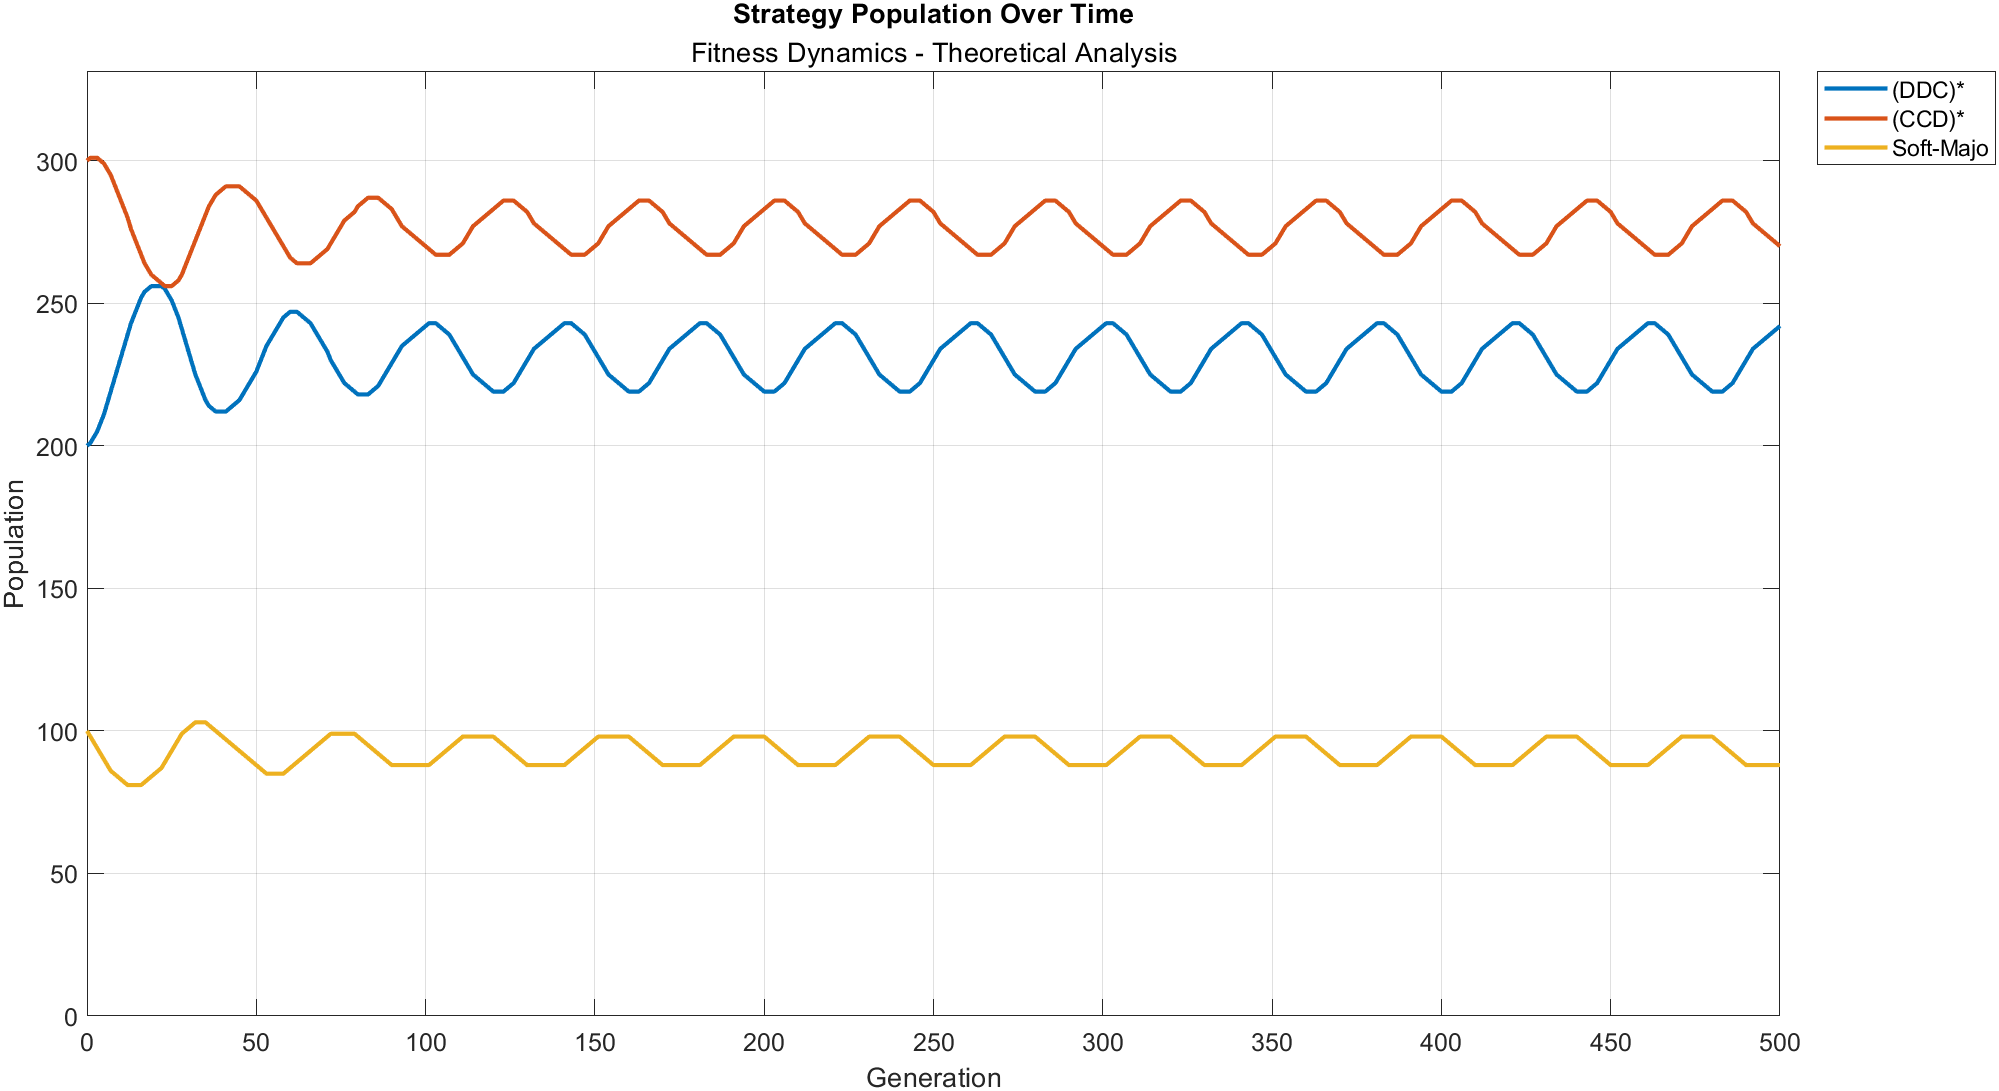
\includegraphics[width=\linewidth]{Figures Fitness Dynamics/example11b.png}
        \caption{Θεωρητικό εξελικτικό πρωτάθλημα}
        \label{fig:fig_fit_11b_b}
    \end{subfigure}
    \hfill
    \begin{subfigure}[b]{0.5\linewidth}
        \centering
        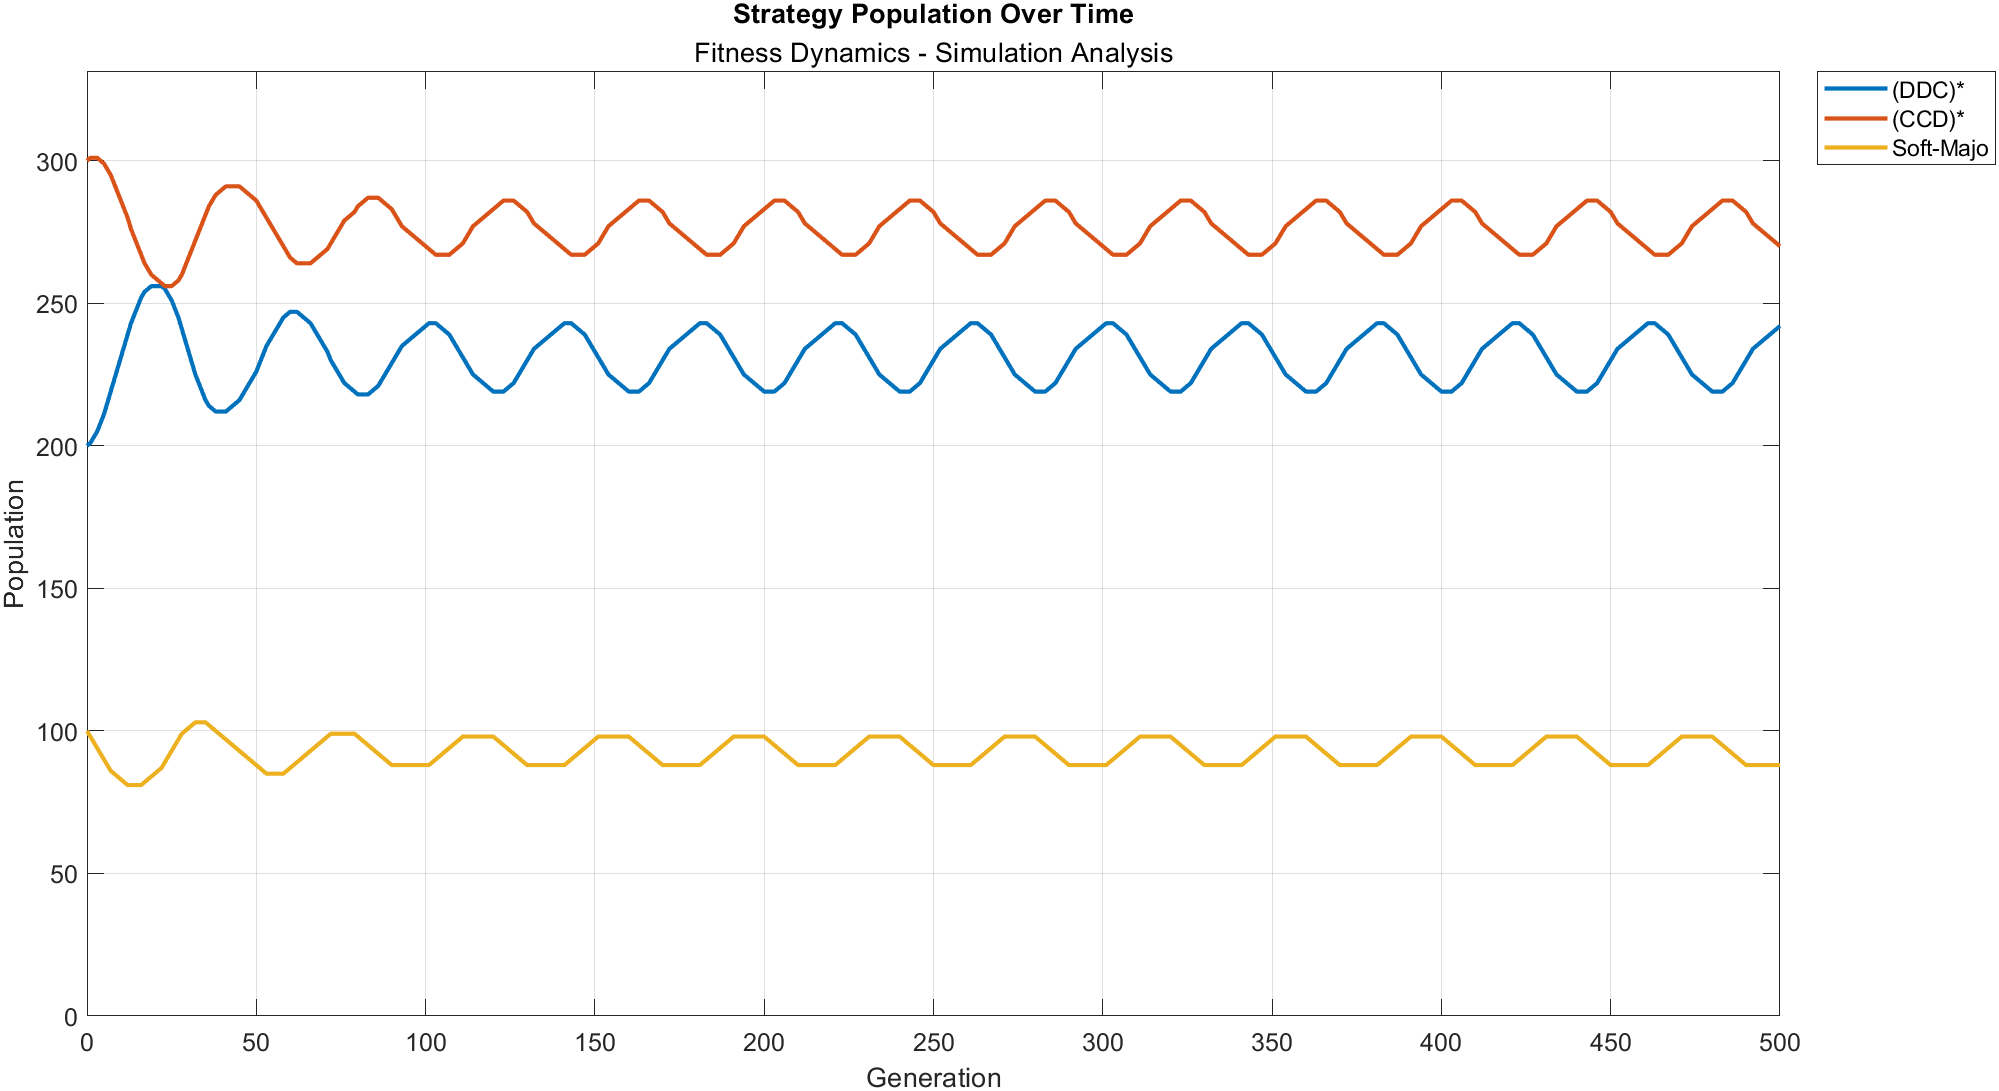
\includegraphics[width=\linewidth]{Figures Fitness Dynamics/example11b-sim.png}
        \caption{Προσομοίωση εξελικτικού πρωταθλήματος}
        \label{fig:fig_fit_11b_c}
        
    \end{subfigure}

    \caption{Αποτελέσματα πειράματος 11β - \foreignlanguage{english}{Script: example11b.m}}
    \label{fig:fig_fit_11b}
\end{figure}

\subsubsection*{Δεύτερο πείραμα}
Στο δεύτερο πείραμα συγκρίνουμε την μεθόδο της στρογγυλοποίησης με τον πολλαπλασιασμό των πληθυσμών κατά μια σταθερά για την ανακατανομή του πληθυσμού. Στα Σχήματα \ref{fig:fig_fit_12a} και \ref{fig:fig_fit_12b} παρουσιάζονται τα αποτελέσματα του εξελικτικού πρωταθλήματος για τις στρατηγικές \foreignlanguage{english}{per\_ccd, per\_ddc} και \foreignlanguage{english}{soft\_majo} με αρχικούς πληθυσμούς 450, 1000 και 100 αντίστοιχα. Στο πρώτο πρωτάθλημα χρησιμοποιούμε την μέθοδο της στραγγυλοποίησης ενώ στο δεύτερο πρωτάθλημα διαιρούμε όλους τους πληθυσμούς με το 10.

Η θεωρητική ανάλυση προβλέπει ότι η στρογγυλοποίηση οδηγεί σε αποσβεννυμένη ταλάντωση, ενώ η διαίρεση των πληθυσμών με το 10 παράγει μια αυξανόμενη ταλάντωση.
Στο πρώτο πρωτάθλημα, η προσομοίωση συμφωνεί με τις θεωρητικές προβλέψεις, ωστόσο το γράφημα της θεωρητικής ανάλυσης παρουσιάζει εξασθενημένη και όχι περιοδική ταλάντωση.
Στο δεύτερο πρωτάθλημα, και οι δύο προσομοιώσεις εμφανίζουν περιοδικές ταλαντώσεις, σε αντίθεση με το αναμενόμενο αποτέλεσμα της θεωρητικής ανάλυσης, η οποία προέβλεπε εξασθένηση των διακυμάνσεων.


\begin{figure}[H]
    \centering

    \begin{subfigure}[b]{0.5\linewidth}
        \centering
        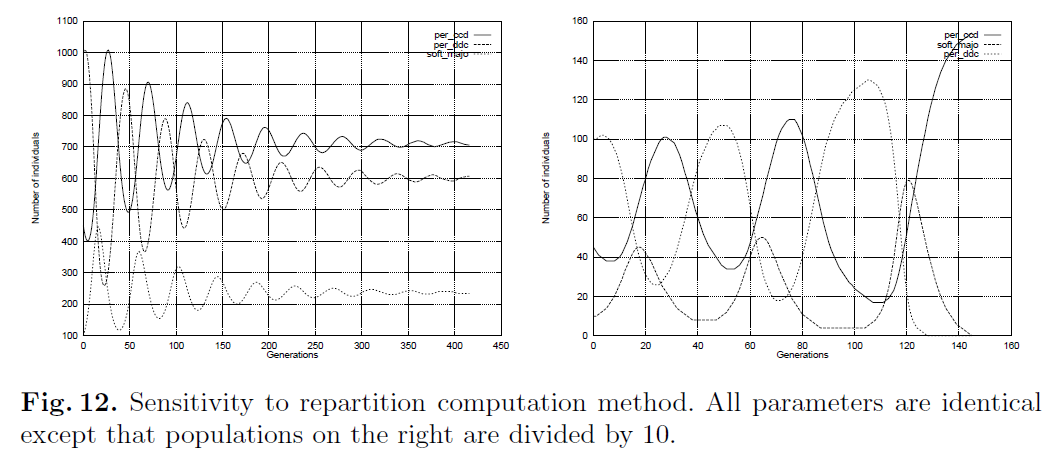
\includegraphics[width=\linewidth]{Figures Fitness Dynamics/12.png}
        \caption{Θεωρητικό αποτέλεσμα από προηγούμενη δημοσίευση. \textit{Πηγή:} \protect\cite{mathieu1999}}
        \label{fig:fig_fit_12_a}
    \end{subfigure}
    \hfill
    \begin{subfigure}[b]{0.5\linewidth}
        \centering
        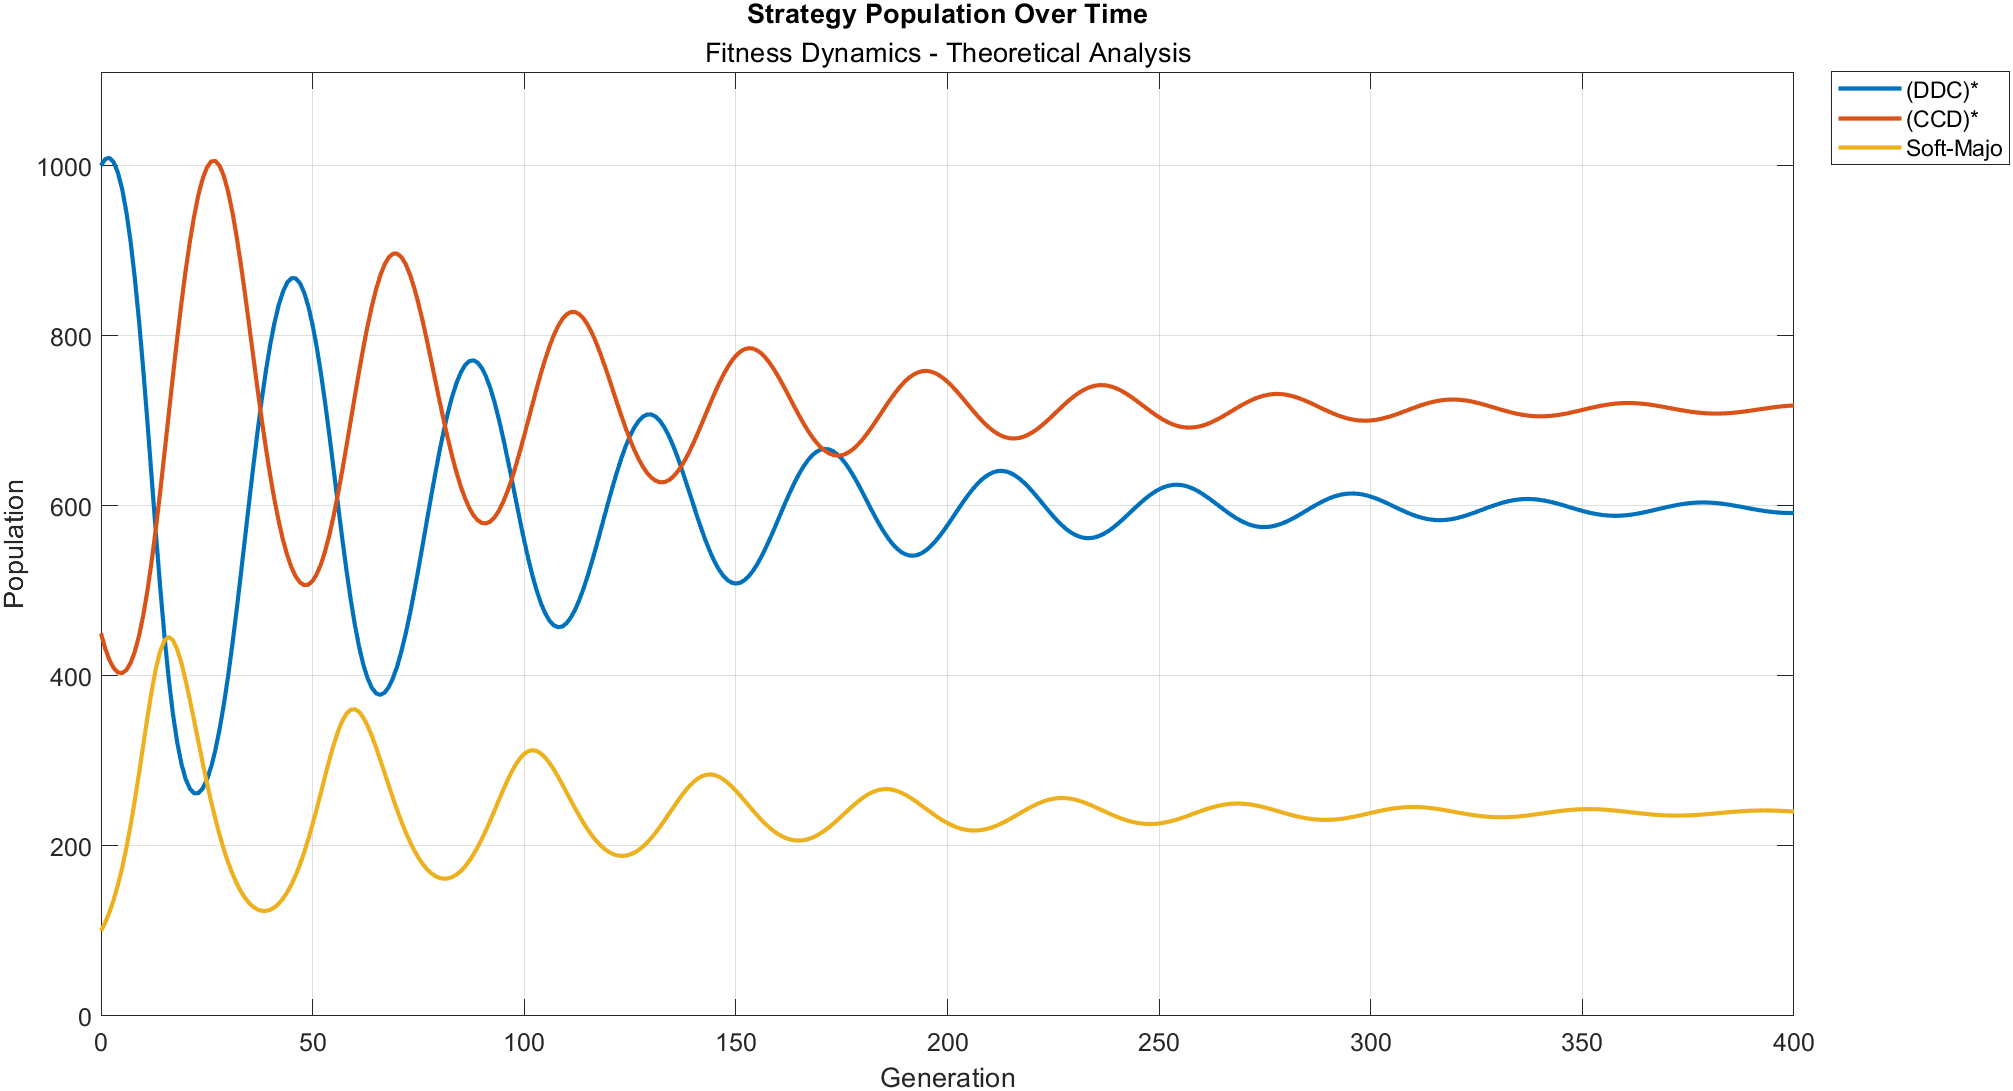
\includegraphics[width=\linewidth]{Figures Fitness Dynamics/example12a.png}
        \caption{Θεωρητικό εξελικτικό πρωτάθλημα}
        \label{fig:fig_fit_12a_b}
    \end{subfigure}
    \hfill
    \begin{subfigure}[b]{0.5\linewidth}
        \centering
        \includegraphics[width=\linewidth]{Figures Fitness Dynamics/example12a-sim.png}
        \caption{Προσομοίωση εξελικτικού πρωταθλήματος}
        \label{fig:fig_fit_12a_c}
        
    \end{subfigure}

    \caption{Αποτελέσματα πειράματος 12α - \foreignlanguage{english}{Script: example12a.m}}
    \label{fig:fig_fit_12a}
\end{figure}

\begin{figure}[H]
    \centering

    \begin{subfigure}[b]{0.5\linewidth}
    \centering
    \includegraphics[width=\linewidth]{Figures Fitness Dynamics/12.png}
    \caption{Θεωρητικό αποτέλεσμα από προηγούμενη δημοσίευση. \textit{Πηγή:} \protect\cite{mathieu1999}}
    \end{subfigure}
    \hfill
    \begin{subfigure}[b]{0.5\linewidth}
        \centering
        \includegraphics[width=\linewidth]{Figures Fitness Dynamics/example12b.png}
        \caption{Θεωρητικό εξελικτικό πρωτάθλημα}
        \label{fig:fig_fit_12b_b}
    \end{subfigure}
    \hfill
    \begin{subfigure}[b]{0.5\linewidth}
        \centering
        \includegraphics[width=\linewidth]{Figures Fitness Dynamics/example12b-sim.png}
        \caption{Προσομοίωση εξελικτικού πρωταθλήματος}
        \label{fig:fig_fit_12b_c}
        
    \end{subfigure}

    \caption{Αποτελέσματα πειράματος 12β - \foreignlanguage{english}{Script: example12b.m}}
    \label{fig:fig_fit_12b}
\end{figure}
\newpage
\subsection{Συμπεράσματα}
Με βάση τα παραπάνω πειράματα, συμπεραίνουμε ότι η εξέλιξη ενός εξελικτικού πρωταθλήματος με \foreignlanguage{english}{Fitness Dynamics} ποικίλλει ανάλογα με τις στρατηγικές που χρησιμοποιούνται. Παράγοντες όπως το μέγεθος του πληθυσμού, η διάρκεια του παιχνιδιού, οι σταθερές στον πίνακα απολαβών, καθώς και η μέθοδος ανακατανομής του πληθυσμού, μπορούν να επηρεάσουν σημαντικά την πορεία και τη δυναμική του πρωταθλήματος.

Όσον αφορά τα αποτελέσματα που προέκυψαν από τις προσομοιώσεις μας, παρατηρείται ότι, στις περισσότερες περιπτώσεις, ευθυγραμμίζονται με εκείνα της δημοσίευσης \cite{mathieu1999}. Αντίθετα, τα αποτελέσματα της θεωρητικής ανάλυσης συχνά αποκλίνουν, παρουσιάζοντας συνήθως μια εξασθενημένη ταλάντωση. Αυτή η απόκλιση στα αποτελέσματα οφείλεται στην διαφορά της ανακατανομής των πληθυσμών στο τέλος κάθε γενιάς. Στην δική μας θεωρητική ανάλυση επιτρέπουμε τους πληθυσμούς να πάρουν μη ακέραιες τιμές κάτι που δεν συμβαίνει στην δημοσίευση \cite{mathieu1999}. Αντίθετα στην προσομοίωση που χρησιμοποιούμε την συνάρτηση $pop\_redistribute$ για να λάβουμε ακέραιους πληθυσμούς τα αποτελέσματα είναι παρόμοια.

\newpage
\section{\foreignlanguage{english}{Imitation Dynamics}}
\subsection{Διαδικασία Εξέλιξης}
Στην περίπτωση που χρησιμοποιούμε \foreignlanguage{english}{Imitation Dynamics}, στο τέλος κάθε γενιάς επιλέγεται από τον πληθυσμό ένας προκαθορισμένος αριθμός παικτών (στους οποίους από εδώ και στο εξής θα αναφερόμαστε ως \foreignlanguage{english}{"Imitators"}) οι οποίοι αλλάζουν την στρατηγική τους και από μια μη βέλτιστη, πλέον υιοθετούν μια βέλτιστη (ως προς την συνολική απόδοση αυτής στην περασμένη γενιά).

Θυμίζουμε πως η συνολική απόδοση κάθε στρατηγικής στο τέλος μιας γενιάς ορίζεται ως το άθροισμα των συγκομιδών κάθε παίκτη αυτής της στρατηγικής, από τις συναντήσεις που είχε με όλους τους άλλους παίκτες στην γενιά. Αυτές οι συνολικές αποδόσεις μας βοηθούν να επιμερίσουμε το σύνολο των στρατηγικών σε βέλτιστες και μη ως εξής:
Έστω $S$ το σύνολο των στρατηγικών, $S_{best}$ το σύνολο των βέλτιστων στρατηγικών, $S - S_{best}$ το σύνολο των μη βέλτιστων στρατηγικών και $A_i^j$ η συνολική απόδοση της στρατηγικής $i \in S$ στο τέλος της γενιάς $j$ (δηλαδή $A_i^j = \sum_{n \in i} g(n)$). Τότε
\begin{equation}
    \label{beststrats}
    S_{best}=\{s \in S \mid A_s^j \geq A_i^j \hspace{0.2 cm} \forall i \in S\}
\end{equation}
Έπειτα θέλουμε να επιλέξουμε έναν προκαθορισμένο αριθμό παικτών που στην περασμένη γενιά έπαιξαν με κάποια στρατηγική $i \in S-S_{best}$. Καθένας από αυτούς θα επιλέξει τυχαία (κι ομοιόμορφα) μία από τις ισοδύναμα βέλτιστες στρατηγικές $s \in S_{best}$ για να την υιοθετήσει στην ερχόμενη γενιά. Πρέπει να σημειωθεί πως σε περίπτωση που οι παίκτες μη βέλτιστων στρατηγικών είναι λιγότεροι σε πλήθος από τον ζητούμενο αριθμό \foreignlanguage{english}{Imitators}, τότε θα επαναπροσδιορίζεται ο αριθμός των \foreignlanguage{english}{Imitators} ως το πλήθος των παικτών μη βέλτιστων στρατηγικών. Με απλά λόγια, θα φτάσουμε κάποια στιγμή στο σημείο όπου όλοι οι εναπομείναντες παίκτες μη βέλτιστων στρατηγικών θα υιοθετήσουν την βέλτιστη και τότε δεν θα υπάρχει μεταβολή στον πληθυσμό αφού όλοι οι παίκτες θα έχουν υιοθετήσει μια μοναδική στρατηγική, ή περισσότερες που είναι όμως ισοδύναμα βέλτιστες. Επαναλαμβάνουμε τα παραπάνω βήματα για προκαθορισμένο αριθμό γενεών.
\begin{algorithm}[H]
\caption{Εξέλιξη με \foreignlanguage{english}{Imitation Dynamics}}
\label{alg:ImitationDyns}
\begin{algorithmic}[1]
\REQUIRE Αριθμός παικτών $N$, πίνακας απολαβών παιγνίου $B$, αριθμός γύρων ανά συνάντηση $T$, σύνολο στρατηγικών $S$, αριθμός γενεών $J$, αρχική κατανομή πληθυσμού $POP_0$, αριθμός \foreignlanguage{english}{Imitators} σε κάθε γενιά $K$
\STATE Ανάθεση στρατηγικής σε κάθε παίκτη σύμφωνα με το $POP_0$
\FOR{κάθε γενιά $j = 1$ έως $J$}
    \FOR{κάθε ζεύγος παικτών $(i, k) \in \{1,2,\dots,N\}\times\{1,2,\dots,N\}$ με $i \ne k$}
        \STATE Οι παίκτες $i$ και $k$ παίζουν ένα επαναληπτικό ΔΦ με $T$ γύρους
        \STATE Καταγραφή της συνολικής απόδοσης κάθε παίκτη από όλα τα παιχνίδια
    \ENDFOR
    \FOR{κάθε παίκτη $n$}
        \STATE $g(n) \gets$ το άθροισμα αποδόσεων του παίκτη $n$ από όλα τα παιχνίδια της γενιάς
    \ENDFOR
    \FOR{κάθε στρατηγική $s$}
        \STATE $A_s^j \gets \sum_{n \in s} g(n)$
    \ENDFOR
    \STATE $S_{best}=\{s \in S \mid A_s^j \geq A_i^j \hspace{0.2 cm} \forall i \in S\}$
    \STATE Αντίγραψε τον πληθυσμό της περασμένης γενιάς στον πληθυσμό της επόμενης
    \STATE $K_{actual} = min(K,$ συνολικό πλήθος παικτών μη βέλτιστων στρατηγικών$)$
    \STATE Επίλεξε από τον πληθυσμό της επόμενης γενιάς $K_{actual}$ παίκτες που ακολουθούν κάποια στρατηγική $i \in S-S_{best}$
    \STATE Για αυτούς τους παίκτες όρισε την στρατηγική τους σε μια τυχαία $s \in S_{best}$
\ENDFOR
    \end{algorithmic}
\end{algorithm}
\subsection{Μαρκοβιανή Ανάλυση}
Έστω ότι ορίζουμε ως κατάσταση την κατανομή των παικτών σε κάθε στρατηγική για μια συγκεκριμένη γενιά. Τότε η κατάσταση στην επόμενη γενιά μετά τις $K$ μιμήσεις έχει την μαρκοβιανή ιδιότητα αφού εξαρτάται μόνο από την τρέχουσα κατάσταση και όχι τις προηγούμενες. Θέλουμε να βρούμε λοιπόν τις πιθανότητες μετάβασης από μια τρέχουσα κατάσταση σε μια επόμενη, ώστε να μπορούμε να περιγράψουμε πλήρως την μαρκοβιανή αλυσίδα.
\begin{algorithm}[H]
\caption{Υπολογισμός Πιθανοτήτων Μεταβάσεων Μαρκοβιανής Αλυσίδας}
\label{alg:StateTransProbs}
\begin{algorithmic}[1]
\REQUIRE Πίνακας απολαβών παιγνίου $B$, αριθμός γύρων ανά συνάντηση $T$, σύνολο στρατηγικών $Strategies$, αριθμός γενεών $J$, αρχική κατανομή πληθυσμού $POP_0$, αριθμός \foreignlanguage{english}{Imitators} σε κάθε γενιά $K$

\STATE Υπολόγισε όλες τις πιθανές καταστάσεις $S$, δηλαδή τις πιθανές κατανομές του πλήθους παικτών στις στρατηγικές.
\FOR{κατάσταση $s = 1:S$}
\STATE Βρες την συνολική απόδοση κάθε στρατηγικής στην κατάσταση $s$
\STATE Βρες τα σύνολα των βέλτιστων και μη βέλτιστων στρατηγικών, όπως τα περιγράψαμε στην \ref{beststrats}
\IF{$K<sum_n($ παίκτης $n$ με στρατηγική $Pn \in S - S_{best})$}
\STATE $K=sum_n($ παίκτης $n$ με στρατηγική $Pn \in S - S_{best})$
\ENDIF
\FOR{κάθε υποψήφια επόμενη κατάσταση $t = 1:S$}
\STATE Υπολόγισε το διάνυσμα διαφορών μεταξύ των δύο καταστάσεων αφαιρώντας $t-s$
\STATE Από αυτό βρες πόσοι παίκτες μιμήθηκαν μια βέλτιστη στρατηγική $(G)$ και πόσοι εγκατέλειψαν μια μη βέλτιστη ($L$)
\STATE Έλεγξε αν η μετάβαση $s\xrightarrow{} t$ είναι έγκυρη. Πρέπει $G=L=K$ με $G, L \geq 0$
\IF{η μετάβαση $s \xrightarrow{}t$ δεν είναι έγκυρη}
\STATE $Pr(s\xrightarrow[]{}t)=0$, συνέχισε για επόμενο $t$
\ELSE
\STATE Υπολόγισε την πιθανότητα $p\_select$ να επιλέξουμε $K$ συγκεκριμένους παίκτες από αυτούς με κάποια μη βέλτιστη στρατηγική. Η πιθανότητα ακολουθεί υπεργεωμετρική κατανομή.
\STATE Υπολόγισε την πιθανότητα $p\_assign$ να αναθέσουμε αυτούς τους $K$ παίκτες σε κάποια από τις βέλτιστες στρατηγικές. Η πιθανότητα ακολουθεί πολυωνυμική κατανομή πολλών μεταβλητών.
\STATE Η πιθανότητα της μετάβασης $Pr(s\xrightarrow[]{}t)=p\_select \times p\_assign$
\ENDIF
\ENDFOR
\ENDFOR
\ENSURE Πίνακας με την πιθανότητα κάθε μετάβασης από μια σύνθεση πληθυσμού σε άλλη
    \end{algorithmic}
\end{algorithm}

\subsection{Πειράματα}
Δοκιμάσαμε να τρέξουμε μερικά πειράματα (τα \foreignlanguage{english}{Matlab Scripts} των οποίων μπορούν να βρεθούν στον φάκελο \foreignlanguage{english}{"examples/Scripts Imitation Dynamics"}) τα οποία για κάποιες παραμέτρους που ρυθμίζουμε εμείς (στρατηγικές και αρχικοί πληθυσμοί αυτών, σύνολο παικτών, πίνακας απολαβών παιγνίου) υπολογίζουν:
\begin{itemize}
    \item Τον πίνακα πιθανοτήτων μετάβασης μεταξύ δύο καταστάσεων, τον οποίον απεικονίζουμε με έναν κατευθυνόμενο γράφο, όπου οι κόμβοι είναι οι καταστάσεις και οι ακμές συμβολίζουν μια μετάβαση με μη μηδενική πιθανότητα (η πραγματική πιθανότητα δεν καταγράφεται αλλά υπάρχει στον πίνακα $P$). Παράλληλα δημιουργούμε κι ένα υπόμνημα που αντιστοιχίζει τον αριθμό μιας κατάστασης στην κατανομή πληθυσμού που αυτή αντιπροσωπεύει (\foreignlanguage{english}{State Map: State ID $\xrightarrow{}$ State Vector})
    \item Την εξέλιξη του πληθυσμού κάθε στρατηγικής ως προς τις γενιές της προσομοίωσης.
\end{itemize}
Σε όλα τα πειράματα χρησιμοποιήσαμε 3 στρατηγικές και έτσι εφόσον ο συνολικός πληθυσμός παραμένει σταθερός μπορούμε να χρησιμοποιήσουμε τους 2 άξονες για να δεικτοδοτήσουμε τους πληθυσμούς 2 από των 3 στρατηγικών σε κάθε κατάσταση, συγκεκριμένα της 2ης και της 3ης κάθε φορά, αφού ο πληθυσμός της 1ης μπορεί να βρεθεί από τον συνολικό πληθυσμό αφαιρώντας το άθροισμα των άλλων 2. Επίσης εφόσον έχουμε 3 στρατηγικές χρησιμοποιούμε χρωματική κωδικοποίηση στους κόμβους του γράφου μεταβάσεων, με τα 'καθαρά' χρώματα Κόκκινο, Πράσινο και Μπλε να αντιχτοιχούν σε καταστάσεις καταβόθρες (μια στρατηγική έχει όλους τους παίκτες οπότε δεν μπορούμε ποτέ να ξεφύγουμε από αυτήν την κατάσταση), ενώ άλλες καταστάσεις με μεικτούς πληθυσμούς προκύπτουν από αντίστοιχους συνδυασμούς χρωμάτων ανάλογα με την σύνθεσή τους. Τέλος έχουμε αφαιρέσει τις ακμές ανακύκλωσης από μια κατάσταση στον εαυτό της για να είναι πιο καθαρό το γράφημα σε περίπτωση μεγαλύτερου πλήθους παικτών.
Σε όλα τα πειράματα, εκτός αν αναφέρεται διαφορετικά, χρησιμοποιήσαμε $T=1000$ γύρους ανά συνάντηση δύο παικτών, $J=10$ γενιές εξέλιξης, $K=1$ \foreignlanguage{english}{imitator} και πίνακα απολαβών [S=0, P=1, R=3, T=5]. Σε κάποια πειράματα τροποποιήσαμε τον πίνακα απολαβών διατηρώντας ωστόσο την διάταξη $S<P<R<T$


Στο πείραμα 13 χρησιμοποιούμε τις στρατηγικές \foreignlanguage{english}{TFT, (CD)*, (DDC)*} με 1 παίκτη σε κάθε μια αρχικά. Παρατηρούμε στο σχήμα \ref{fig:fig13-sim} πως η $(DDC)^*$ επικρατεί εύκολα των άλλων 2, ενώ παρατηρούμε πως στον γράφο μεταβάσεων \ref{fig:fig13} ότι 3 από τις 7 μεικτές καταστάσεις καταλήγουν στην 'καθαρή' κατάσταση με παίκτες μόνο της $(DDC)^*$, ενώ οι άλλες 4 μεικτές μοιράζονται στις άλλες 2 'καθαρές' καταστάσεις.
\begin{figure}[H]
    \centering

    \begin{subfigure}[b]{0.45\textwidth}
        \includegraphics[width=\linewidth]{Figures Imitation Dynamics/example13.png}
        \caption{Κατευθυνόμενος γράφος μεταβάσεων}
        \label{fig:fig13}
    \end{subfigure}
    \hfill
    \begin{subfigure}[b]{0.45\textwidth}
        \includegraphics[width=\linewidth]{Figures Imitation Dynamics/example13-sim.png}
        \caption{Εξέλιξη πληθυσμού ανά γενιά}
        \label{fig:fig13-sim}
    \end{subfigure}

    \caption{Πείραμα 13 - \foreignlanguage{english}{Script: example13.m}}
    \label{fig:example13}
\end{figure}

Για το πείραμα 14 θέλουμε να βρούμε κάποια άλλη στρατηγική που να μπορεί να ξεπεράσει την $(DDC)^*$. Για αυτό στην θέση της $TFT$ που στο πείραμα 13 ήταν η χειρότερη βάζουμε την $Gradual$ με επίσης 1 παίκτη. Φαίνεται από το \ref{fig:fig14-sim} πως η $Gradual$ όντως καταφέρνει να επιβληθεί της $(DDC)^*$. Μάλιστα στον γράφο μεταβάσεων \ref{fig:fig14} στην συνεκτική συνιστώσα της 'καθαρής' $Gradual$ ανήκουν 4 από τις 7 μεικτές καταστάσεις.
\begin{figure}[H]
    \centering

    \begin{subfigure}[b]{0.45\textwidth}
        \includegraphics[width=\linewidth]{Figures Imitation Dynamics/example14.png}
        \caption{Κατευθυνόμενος γράφος μεταβάσεων}
        \label{fig:fig14}
    \end{subfigure}
    \hfill
    \begin{subfigure}[b]{0.45\textwidth}
        \includegraphics[width=\linewidth]{Figures Imitation Dynamics/example14-sim.png}
        \caption{Εξέλιξη πληθυσμού ανά γενιά}
        \label{fig:fig14-sim}
    \end{subfigure}

    \caption{Πείραμα 14 - \foreignlanguage{english}{Script: example14.m}}
    \label{fig:example14}
\end{figure}

Για το πείραμα 15 χρησιμοποιούμε τις ίδιες παραμέτρους και στρατηγικές με το πείραμα 13 με μόνη διαφορά ότι χρησιμοποιούμε διαφορετικό πίνακα απολαβών παιγνίου $[S=1, P=2, R=3.5, T=4]$. Ουσιαστικά μειώνουμε το εύρος των απολαβών από το 0-5 στο 1-4. Παρόλα αυτά στο \ref{fig:example15} δεν φαίνεται να υπάρχει καμία διαφορά σε σχέση με το \ref{fig:example13}.
\begin{figure}[H]
    \centering

    \begin{subfigure}[b]{0.45\textwidth}
        \includegraphics[width=\linewidth]{Figures Imitation Dynamics/example15.png}
        \caption{Κατευθυνόμενος γράφος μεταβάσεων}
        \label{fig:fig15}
    \end{subfigure}
    \hfill
    \begin{subfigure}[b]{0.45\textwidth}
        \includegraphics[width=\linewidth]{Figures Imitation Dynamics/example15-sim.png}
        \caption{Εξέλιξη πληθυσμού ανά γενιά}
        \label{fig:fig15-sim}
    \end{subfigure}

    \caption{Πείραμα 15 - \foreignlanguage{english}{Script: example15.m}}
    \label{fig:example15}
\end{figure}

Στο πείραμα 16 χρησιμοποιούμε τις ίδιες βασικές στρατηγικές (\foreignlanguage{english}{TFT, (CD)*, (DDC)*}) αλλά τώρα αυξάνουμε τον συνολικό αριθμό παικτών από 3 σε 5. Επειδή έχουμε 3 στρατηγικές αναγκαστικά μια θα πρέπει να έχει 1 παίκτη αρχικά, ενώ οι άλλες 2. Επιλέγουμε η $(DDC)^*$ να έχει 1 παίκτη αφού στο πείραμα 13 ήταν η καλύτερη και θέλουμε να δούμε εάν πάλι θα καταφέρει να υπερισχύσει με έναν παίκτη λιγότερο στην αρχή. Στο \ref{fig:fig16-sim} αυτό δεν φαίνεται να ισχύει και η $TFT$ κυριαρχεί μετά από 3 γενιές.
\begin{figure}[H]
    \centering

    \begin{subfigure}[b]{0.45\textwidth}
        \includegraphics[width=\linewidth]{Figures Imitation Dynamics/example16.png}
        \caption{Κατευθυνόμενος γράφος μεταβάσεων}
        \label{fig:fig16}
    \end{subfigure}
    \hfill
    \begin{subfigure}[b]{0.45\textwidth}
        \includegraphics[width=\linewidth]{Figures Imitation Dynamics/example16-sim.png}
        \caption{Εξέλιξη πληθυσμού ανά γενιά}
        \label{fig:fig16-sim}
    \end{subfigure}

    \caption{Πείραμα 16 - \foreignlanguage{english}{Script: example16.m}}
    \label{fig:example16}
\end{figure}

Στο πείραμα 17 για $N=5$ παίκτες δοκιμάζουμε ένα εντελώς διαφορετικό σύνολο στρατηγικών, \foreignlanguage{english}{AllD, TFT, Prober} με την $TFT$ να ξεκινάει με παίκτη λιγότερο. Στο \ref{fig:fig17-sim} η $Prober$ φαίνεται να κυριαρχεί μετά από 5 γενιές.
\begin{figure}[H]
    \centering

    \begin{subfigure}[b]{0.45\textwidth}
        \includegraphics[width=\linewidth]{Figures Imitation Dynamics/example17.png}
        \caption{Κατευθυνόμενος γράφος μεταβάσεων}
        \label{fig:fig17}
    \end{subfigure}
    \hfill
    \begin{subfigure}[b]{0.45\textwidth}
        \includegraphics[width=\linewidth]{Figures Imitation Dynamics/example17-sim.png}
        \caption{Εξέλιξη πληθυσμού ανά γενιά}
        \label{fig:fig17-sim}
    \end{subfigure}

    \caption{Πείραμα 17 - \foreignlanguage{english}{Script: example17.m}}
    \label{fig:example17}
\end{figure}

Στο πείραμα 18 χρησιμοποιούμε ξανά το σύνολο στρατηγικών \foreignlanguage{english}{TFT, (CD)*, (DDC)*} με $N=5$ παίκτες και την $(DDC)^*$ με παίκτη λιγότερο, ενώ ορίζουμε διαφορετικό πίνακα απολαβών $[S=0, P=1, R=2, T=10]$. Θέλουμε να δούμε εάν το πολύ υψηλό $T=10$ σε σχέση με τις άλλες απολαβές μπορεί να βοηθήσει την $(DDC)^*$ να υπερισχύσει έστω και με αριθμητικό μειονέκτημα. Κάτι τέτοιο δεν φαίνεται να συμβαίνει στο \ref{fig:fig18-sim} αφού η $TFT$ κυριαρχεί μετά από 4 γενιές.
\begin{figure}[H]
    \centering

    \begin{subfigure}[b]{0.45\textwidth}
        \includegraphics[width=\linewidth]{Figures Imitation Dynamics/example18.png}
        \caption{Κατευθυνόμενος γράφος μεταβάσεων}
        \label{fig:fig18}
    \end{subfigure}
    \hfill
    \begin{subfigure}[b]{0.45\textwidth}
        \includegraphics[width=\linewidth]{Figures Imitation Dynamics/example18-sim.png}
        \caption{Εξέλιξη πληθυσμού ανά γενιά}
        \label{fig:fig18-sim}
    \end{subfigure}

    \caption{Πείραμα 18 - \foreignlanguage{english}{Script: example18.m}}
    \label{fig:example18}
\end{figure}

Στο πείραμα 19 θεωρούμε ξανά το σύνολο στρατηγικών \foreignlanguage{english}{TFT, (CD)*, (DDC)*} με $N=6$ αυτή τη φορά και ίσα μοιρασμένους παίκτες στις 3 στρατηγικές. Βλέπουμε στο \ref{fig:fig19-sim} πως η $TFT$ κυριαρχεί μετά από 8 γενιές με την $(CD)^*$ να είναι 2η καλύτερη. Αυτό μπορεί να συγκριθεί με το πείραμα 13 όπου για τις ίδιες στρατηγικές είχαμε πάλι ίσο διαμερισμό παικτών στις στρατηγικές, αλλά τότε η διάταξη των στρατηγικών προέκυψε αντίθετα (βλ. \ref{fig:fig13-sim}. Βλέπουμε λοιπόν πως ο διπλασιασμός του συνολικού πλήθους παικτών αντέστρεψε την επίδοση των στρατηγικών.
\begin{figure}[H]
    \centering

    \begin{subfigure}[b]{0.45\textwidth}
        \includegraphics[width=\linewidth]{Figures Imitation Dynamics/example19.png}
        \caption{Κατευθυνόμενος γράφος μεταβάσεων}
        \label{fig:fig19}
    \end{subfigure}
    \hfill
    \begin{subfigure}[b]{0.45\textwidth}
        \includegraphics[width=\linewidth]{Figures Imitation Dynamics/example19-sim.png}
        \caption{Εξέλιξη πληθυσμού ανά γενιά}
        \label{fig:fig19-sim}
    \end{subfigure}

    \caption{Πείραμα 19 - \foreignlanguage{english}{Script: example19.m}}
    \label{fig:example19}
\end{figure}

Για το πείραμα 20 προσθέτουμε στις ίδιες στρατηγικές \foreignlanguage{english}{TFT, (CD)*, (DDC)*} έναν ακόμη παίκτη, στην $(DDC)^*$ που αναδείχθηκε η χειρότερη στο πείραμα 19, οπότε τώρα έχουμε $N=7$ παίκτες. Όπως φαίνεται στο \ref{fig:fig20-sim} αυτός ο επιπλέον παίκτης βοηθάει την $(DDC)^*$ να κυριαρχήσει μόλις σε 5 γενιές.
\begin{figure}[H]
    \centering

    \begin{subfigure}[b]{0.45\textwidth}
        \includegraphics[width=\linewidth]{Figures Imitation Dynamics/example20.png}
        \caption{Κατευθυνόμενος γράφος μεταβάσεων}
        \label{fig:fig20}
    \end{subfigure}
    \hfill
    \begin{subfigure}[b]{0.45\textwidth}
        \includegraphics[width=\linewidth]{Figures Imitation Dynamics/example20-sim.png}
        \caption{Εξέλιξη πληθυσμού ανά γενιά}
        \label{fig:fig20-sim}
    \end{subfigure}

    \caption{Πείραμα 20 - \foreignlanguage{english}{Script: example20.m}}
    \label{fig:example20}
\end{figure}

Για το πείραμα 21, εφόσον βλέπουμε οι στρατηγικές $TFT$ και $(DDC)^*$ εναλλάσσονται ως οι νικήτριες των προσομοιώσεων στα προηγούμενα πειράματα διατηρούμε το $N=7$ αλλά αφαιρούμε έναν παίκτη από την $(CD)^*$ και τον αναθέτουμε αρχικά στην $TFT$. Βλέπουμε στο \ref{fig:fig21-sim} πως με ίσους πληθυσμούς η $TFT$ επικρατεί σε 7 γενιές. 
\begin{figure}[H]
    \centering

    \begin{subfigure}[b]{0.45\textwidth}
        \includegraphics[width=\linewidth]{Figures Imitation Dynamics/example21.png}
        \caption{Κατευθυνόμενος γράφος μεταβάσεων}
        \label{fig:fig21}
    \end{subfigure}
    \hfill
    \begin{subfigure}[b]{0.45\textwidth}
        \includegraphics[width=\linewidth]{Figures Imitation Dynamics/example21-sim.png}
        \caption{Εξέλιξη πληθυσμού ανά γενιά}
        \label{fig:fig21-sim}
    \end{subfigure}

    \caption{Πείραμα 21 - \foreignlanguage{english}{Script: example21.m}}
    \label{fig:example21}
\end{figure}

Στο πείραμα 22, πάλι για το σύνολο στρατηγικών \foreignlanguage{english}{TFT, (CD)*, (DDC)*} θεωρούμε $N=9$ παίκτες ίσα μοιρασμένους. Στο \ref{fig:fig22-sim} παρατηρούμε πως η $TFT$ πάλι επικρατεί.
\begin{figure}[H]
    \centering

    \begin{subfigure}[b]{0.45\textwidth}
        \includegraphics[width=\linewidth]{Figures Imitation Dynamics/example22.png}
        \caption{Κατευθυνόμενος γράφος μεταβάσεων}
        \label{fig:fig22}
    \end{subfigure}
    \hfill
    \begin{subfigure}[b]{0.45\textwidth}
        \includegraphics[width=\linewidth]{Figures Imitation Dynamics/example22-sim.png}
        \caption{Εξέλιξη πληθυσμού ανά γενιά}
        \label{fig:fig22-sim}
    \end{subfigure}

    \caption{Πείραμα 22 - \foreignlanguage{english}{Script: example22.m}}
    \label{fig:example22}
\end{figure}

Στο πείραμα 23 διατηρούμε $N=9$, αφαιρούμε έναν παίκτη αρχικά από την $(CD)^*$ και τον μεταφέρουμε στην $(DDC)^*$. Στο \ref{fig:fig23-sim} φαίνεται πως η $(DDC)^*$ επικρατεί σε μόλις 5 γενιές χάρη στο αρχικό αριθμητικό πλεονέκτημα.
\begin{figure}[H]
    \centering

    \begin{subfigure}[b]{0.45\textwidth}
        \includegraphics[width=\linewidth]{Figures Imitation Dynamics/example23.png}
        \caption{Κατευθυνόμενος γράφος μεταβάσεων}
        \label{fig:fig23}
    \end{subfigure}
    \hfill
    \begin{subfigure}[b]{0.45\textwidth}
        \includegraphics[width=\linewidth]{Figures Imitation Dynamics/example23-sim.png}
        \caption{Εξέλιξη πληθυσμού ανά γενιά}
        \label{fig:fig23-sim}
    \end{subfigure}

    \caption{Πείραμα 23 - \foreignlanguage{english}{Script: example23.m}}
    \label{fig:example23}
\end{figure}

Τέλος στο πείραμα 24, αντικαθιστούμε την $TFT\xrightarrow{}AllC$ και μοιράζουμε ίσα τους $N=9$ παίκτες στις 3 στρατηγικές. Επίσης αλλάζουμε τον πίνακα απολαβών του παιγνίου σε $[S=1,P=2,R=3.8,T=4]$ ώστε να ενθαρρύνουμε την από κοινού συνεργασία, αφού το $R \approx T$. Αυτό φαίνεται από το \ref{fig:fig24-sim} πως βοηθάει την $AllC$ να επιβιώσει για 6 γενιές, παρόλα αυτά η $(DDC)^*$ επικρατεί τελικά. 
\begin{figure}[H]
    \centering

    \begin{subfigure}[b]{0.45\textwidth}
        \includegraphics[width=\linewidth]{Figures Imitation Dynamics/example24.png}
        \caption{Κατευθυνόμενος γράφος μεταβάσεων}
        \label{fig:fig24}
    \end{subfigure}
    \hfill
    \begin{subfigure}[b]{0.45\textwidth}
        \includegraphics[width=\linewidth]{Figures Imitation Dynamics/example24-sim.png}
        \caption{Εξέλιξη πληθυσμού ανά γενιά}
        \label{fig:fig24-sim}
    \end{subfigure}

    \caption{Πείραμα 24 - \foreignlanguage{english}{Script: example24.m}}
    \label{fig:example24}
\end{figure}




\subsection{Συμπεράσματα}
Φαίνεται από τα παραπάνω πειράματα πως η αρχική σύνθεση πληθυσμών παίζει σημαντικό ρόλο στην τελική έκβαση της προσομοίωσης μετά από κάποιον αριθμό γενεών. Ακόμη και αριθμητικό πλεονέκτημα 1 παίκτη στην αρχική κατάσταση μπορεί να είναι καθοριστικό για τον νικητή του εξελικτικού πρωταθλήματος κι αυτό είναι λόγω της εξέλιξης μέσω \foreignlanguage{english}{Imitation Dynamics} όπου οι βέλτιστες στρατηγικές πάντα ενισχύονται ενώ οι μη βέλτιστες πάντα εξασθενούν στην πάροδο των γενεών. Οπότε αρκεί για μια στρατηγική να νικήσει στην 1η γενιά (έχοντας για παράδειγμα έστω έναν παραπάνω παίκτη) για να νικήσει σε όλο το εξελικτικό τουρνουά.
Επίσης σημαντικό ρόλο παίζει και το συνολικό πλήθος παικτών, ενώ αλλαγές στον πίνακα απολαβών εφόσον διατηρείται η βασική σχέση $S<P<R<T$ δεν φαίνεται να είναι ικανές να επηρεάσουν το αποτέλεσμα του εξελικτικού πρωταθλήματος.


\section{Γενικότερα συμπεράσματα - Συγκρίσεις}
Παρατηρούμε ότι υπάρχουν σημαντικές διαφορές μεταξύ των δύο τεχνικών αναδιανομής του πληθυσμού μεταξύ γενεών. Η αναδιανομή μέσω \foreignlanguage{english}{Fitness Dynamics} μπορεί παρουσιάσει ταλαντώσεις ή και χάος στην σύνθεση πληθυσμών των στρατηγικών, ενώ μπορεί να απαιτηθεί μεγάλος αριθμός γενεών έως ότου αναδειχθούν σταθερές τάσεις ή μέχρι να φτάσουμε σε σύγκλιση.

Αντιθέτως, η αναδιανομή μέσω \foreignlanguage{english}{Imitation Dynamics} φαίνεται πως οδηγεί σε μονότονες και γραμμικές μεταβολές πληθυσμού, καθώς εκ φύσεως ενισχύει τις ισχυρές στρατηγικές και εξασθενεί τις αδύναμες, πάντα κατά τον σταθερό παράγοντα Κ.

Ουσιαστικά η διαφορά των δύο δυναμικών έγκειται στο γεγονός πως στην \foreignlanguage{english}{Fitness Dynamics} το κέρδος μιας βέλτιστης στρατηγικής σε σχέση με μια μη βέλτιστη είναι ανάλογο της διαφοράς της ισχύος τους (είναι σχετικό). Δηλαδή όσο πιο ισχυρή είναι μια στρατηγική σε σχέση με τις υπόλοιπες τόσο περισσότερο θα ενισχυθεί.
Αυτή η παρατήρηση εξηγεί και τις συχνά απρόβλεπτες συμπεριφορές στην σύνθεση των πληθυσμών.
Αντίθετα στην \foreignlanguage{english}{Imitation Dynamics} δεν έχει σημασία η σχετική, αλλά η απόλυτη διαφορά ισχύος, μεταξύ βέλτιστων και μη-βέλτιστων στρατηγικών. Μια βέλτιστη στρατηγική θα ενισχυθεί το ίδιο (κατά Κ) ανεξάρτητα του πόσο καλύτερη είναι από τις μη-βέλτιστες.
Αυτή η παρατήρηση εξηγεί και την μονοτονική μεταβολή των πληθυσμών.

\chapter{Παραρτήματα}


\section{\foreignlanguage{english}{Documentation}
\label{documentation}}
\selectlanguage{english}


\subsection*{TourTheFit}

\textbf{\foreignlanguage{greek}{Σύνταξη}:}
\begin{verbatim}
[POP, BST, FIT] = TourTheFit(B, Strategies, POP0, T, J)
\end{verbatim}

\textbf{\foreignlanguage{greek}{Περιγραφή:}} \\
\foreignlanguage{greek}{
Πραγματοποιεί την θεωρητική ανάλυση του πρωταθλήματος \foreignlanguage{english}{Axelrod} υπολογίζοντας τους πληθυσμούς κάθε στρατηγικής, τις τιμές \foreignlanguage{english}{Fitness} αυτών και τις καλύτερες σε κάθε γενιά. Χρησιμοποιεί τον αλγόριθμο εξέλιξης \foreignlanguage{english}{Fitness} που περιγράφεται στην δημοσίευση \cite{mathieu1999}.}

\textbf{\foreignlanguage{greek}{Ορίσματα:}}
\begin{itemize}
    \item \texttt{B} – Payoff matrix (2x2)
    \item \texttt{Strategies} – Cell array of strategy names
    \item \texttt{POP0} – Initial population vector
    \item \texttt{T} – Number of rounds per match
    \item \texttt{J} – Number of generations
\end{itemize}

\textbf{\foreignlanguage{greek}{Επιστρέφει}:}
\begin{itemize}
    \item \texttt{POP} – Population matrix (\#strategies × generations)
    \item \texttt{BST} – Best strategy/strategies per generation (names)
    \item \texttt{FIT} – Fitness values per strategy and generation
\end{itemize}

\subsection*{TourSimFit}

\textbf{\foreignlanguage{greek}{Σύνταξη}:}
\begin{verbatim}
[POP, BST, FIT] = TourSimFit(B, Strategies, POP0, T, J)
\end{verbatim}

\textbf{\foreignlanguage{greek}{Περιγραφή:}} \\
\foreignlanguage{greek}{
Πραγματοποιεί την μερική προσομοίωση (προϋπολογίσμένες οι απολαβές κάθε παίκτη για μια συνάντηση, όχι πλήρης προσομοίωση κάθε γύρου) του πρωταθλήματος \foreignlanguage{english}{Axelrod} υπολογίζοντας τους πληθυσμούς κάθε στρατηγικής, τις τιμές \foreignlanguage{english}{Fitness} αυτών και τις καλύτερες σε κάθε γενιά. Χρησιμοποιεί τον αλγόριθμο εξέλιξης \foreignlanguage{english}{Fitness} που περιγράφεται στην δημοσίευση \cite{mathieu1999}.}

\textbf{\foreignlanguage{greek}{Ορίσματα:}}
\begin{itemize}
    \item \texttt{B} – Payoff matrix (2x2)
    \item \texttt{Strategies} – Cell array of strategy names
    \item \texttt{POP0} – Initial population vector
    \item \texttt{T} – Number of rounds per match
    \item \texttt{J} – Number of generations
\end{itemize}

\textbf{\foreignlanguage{greek}{Επιστρέφει}:}
\begin{itemize}
    \item \texttt{POP} – Population matrix (\#strategies × generations)
    \item \texttt{BST} – Best strategy/strategies per generation (names)
    \item \texttt{FIT} – Fitness values per strategy and generation
\end{itemize}

\subsection*{TourTheFit\_Integer\_Populations}

\textbf{\foreignlanguage{greek}{Σύνταξη}:}
\begin{verbatim}
[POP, BST, FIT] = TourTheFit_Integer_Populations(B, Strategies, POP0, T, J)
\end{verbatim}

\textbf{\foreignlanguage{greek}{Περιγραφή:}} \\
\foreignlanguage{greek}{
Όλες οι παράμετροι είναι ίδιες με την \foreignlanguage{english}{TourTheFit} με μόνη διαφορά ότι οι πληθυσμοί στρατηγικών σε κάθε γενιά είναι ακέραιοι αριθμοί που υπολογίζονται με τον αλγόριθμο \ref{alg:PopRedist}.}

\subsection*{TourSimImi}

\textbf{\foreignlanguage{greek}{Σύνταξη}:}
\begin{verbatim}
[POP, BST] = TourSimImi(B, Strategies, POP0, K, T, J)
\end{verbatim}

\textbf{\foreignlanguage{greek}{Περιγραφή:}} \\
\foreignlanguage{greek}{
Πραγματοποιεί την μερική προσομοίωση (προϋπολογίσμένες οι απολαβές κάθε παίκτη για μια συνάντηση, όχι πλήρης προσομοίωση κάθε γύρου) του πρωταθλήματος \foreignlanguage{english}{Axelrod} υπολογίζοντας τους πληθυσμούς κάθε στρατηγικής και τις καλύτερες σε κάθε γενιά. Χρησιμοποιεί τον αλγόριθμο εξέλιξης \foreignlanguage{english}{Imitation} που περιγράφεται στον αλγόριθμο \ref{alg:ImitationDyns}.}

\textbf{\foreignlanguage{greek}{Ορίσματα:}}
\begin{itemize}
    \item \texttt{B} – Payoff matrix (2x2)
    \item \texttt{Strategies} – Cell array of strategy names
    \item \texttt{POP0} – Initial population vector
    \item \texttt{K} – Number of Imitators per generation
    \item \texttt{T} – Number of rounds per match
    \item \texttt{J} – Number of generations
\end{itemize}

\textbf{\foreignlanguage{greek}{Επιστρέφει}:}
\begin{itemize}
    \item \texttt{POP} – Population matrix (\#strategies × generations)
    \item \texttt{BST} – Best strategy/strategies per generation (names)
\end{itemize}

\subsection*{TourTheImi}

\textbf{\foreignlanguage{greek}{Σύνταξη}:}
\begin{verbatim}
P = TourTheImi(B, Strategies, POP0, K, T, J)
\end{verbatim}

\textbf{\foreignlanguage{greek}{Περιγραφή:}} \\
\foreignlanguage{greek}{
Υπολογίζει τον πίνακα πιθανοτήτων μεταβάσεων από μια κατάσταση του πληθυσμού σε μια επόμενη, χρησιμοποιώντας τον αλγόριθμο \ref{alg:StateTransProbs}.}

\textbf{\foreignlanguage{greek}{Ορίσματα:}}
\begin{itemize}
    \item \texttt{B} – Payoff matrix (2x2)
    \item \texttt{Strategies} – Cell array of strategy names
    \item \texttt{POP0} – Initial population vector
    \item \texttt{K} – Number of Imitators per generation
    \item \texttt{T} – Number of rounds per match
    \item \texttt{J} – Number of generations
\end{itemize}

\textbf{\foreignlanguage{greek}{Επιστρέφει}:}
\begin{itemize}
    \item \texttt{P} – Transition Probability Matrix
\end{itemize}

\subsection*{axel}

\textbf{\foreignlanguage{greek}{Σύνταξη}:}
\begin{verbatim}
scores = axel(B, Strategies, Pop, T)
\end{verbatim}

\textbf{\foreignlanguage{greek}{Περιγραφή:}} \\
\foreignlanguage{greek}{
Επιστρέφει την συνολική συγκομιδή όλων των παικτών μετά το τέλος ενός τουρνουά \foreignlanguage{english}{Axelrod} όπου όλοι οι παίκτες συναντιούνται από μια φορά με όλους τους υπόλοιπους.}

\textbf{\foreignlanguage{greek}{Ορίσματα:}}
\begin{itemize}
    \item \texttt{B} – Payoff matrix (2x2)
    \item \texttt{Strategies} – Cell array of strategy names
    \item \texttt{Pop} – Strategy population vector
    \item \texttt{T} – Number of rounds per match
\end{itemize}

\textbf{\foreignlanguage{greek}{Επιστρέφει}:}
\begin{itemize}
    \item \texttt{scores} – Vector of total scores for each player after every possible match
\end{itemize}

\subsection*{axel\_partial}

\textbf{\foreignlanguage{greek}{Σύνταξη}:}
\begin{verbatim}
scores = axel_partial(B, Strategies, Pop, T)
\end{verbatim}

\textbf{\foreignlanguage{greek}{Περιγραφή:}} \\
\foreignlanguage{greek}{
Οι ίδιες παράμετροι με την \foreignlanguage{english}{axel}, με μόνη διαφορά ότι για κάθε πιθανή συνάντηση είναι προϋπολογισμένη η συγκομιδή κάθε παίκτη. Χρησιμοποιείται σε μερικές προσομοιώσεις.}

\subsection*{compositions}

\textbf{\foreignlanguage{greek}{Σύνταξη}:}
\begin{verbatim}
comps = compositions(n, k)
\end{verbatim}

\textbf{\foreignlanguage{greek}{Περιγραφή:}} \\
\foreignlanguage{greek}{
Επιστρέφει όλες τις δυνατές καταστάσεις του πληθυσμού για \foreignlanguage{english}{n} παίκτες και \foreignlanguage{english}{k} στρατηγικές. Χρησιμοποιείται σε \foreignlanguage{english}{Imitation Dynamics}.}

\textbf{\foreignlanguage{greek}{Ορίσματα:}}
\begin{itemize}
    \item \texttt{n} – Total players
    \item \texttt{k} – Number of strategies
\end{itemize}

\textbf{\foreignlanguage{greek}{Επιστρέφει}:}
\begin{itemize}
    \item \texttt{comps} – Matrix of all possible population states
\end{itemize}

\subsection*{ComputePayoffMatrix}

\textbf{\foreignlanguage{greek}{Σύνταξη}:}
\begin{verbatim}
V = ComputePayoffMatrix(Strategies, B, T)
\end{verbatim}

\textbf{\foreignlanguage{greek}{Περιγραφή:}} \\
\foreignlanguage{greek}{
Προϋπολογίζει τον πίνακα συγκομιδών για κάθε δυνατή συνάντηση δύο παικτών}

\textbf{\foreignlanguage{greek}{Ορίσματα:}}
\begin{itemize}
    \item \texttt{B} – Payoff matrix (2x2)
    \item \texttt{Strategies} – Cell array of strategy names
    \item \texttt{T} – Number of rounds per match
\end{itemize}

\textbf{\foreignlanguage{greek}{Επιστρέφει}:}
\begin{itemize}
    \item \texttt{V} – Matrix of total payoffs for every possible match
\end{itemize}

\subsection*{get\_strategy\_move}

\textbf{\foreignlanguage{greek}{Σύνταξη}:}
\begin{verbatim}
move = get_strategy_move(player_strategy, history, player_id)
\end{verbatim}

\textbf{\foreignlanguage{greek}{Περιγραφή:}} \\
\foreignlanguage{greek}{
Επιστρέφει την κίνηση που θα παίξει κάποιος παίκτης δεδομένης της στρατηγικής του και του ιστορικού κινήσεων στο τρέχον παιχνίδι.}

\textbf{\foreignlanguage{greek}{Ορίσματα:}}
\begin{itemize}
    \item \texttt{player\_strategy} – Strategy of the player to move
    \item \texttt{history} – Move history of current match
    \item \texttt{player\_id} – The column of the moves history to examine
\end{itemize}

\textbf{\foreignlanguage{greek}{Επιστρέφει}:}
\begin{itemize}
    \item \texttt{move} – The next move 'C' or 'D'
\end{itemize}

\subsection*{play\_match}

\textbf{\foreignlanguage{greek}{Σύνταξη}:}
\begin{verbatim}
[score1, score2] = play_match(player1, player2, B, T)
\end{verbatim}

\textbf{\foreignlanguage{greek}{Περιγραφή:}} \\
\foreignlanguage{greek}{
Προσομοιώνει την συνάντηση δύο παικτών και επιστρέφει την συγκομιδή του καθενός στο τέλος.}

\textbf{\foreignlanguage{greek}{Ορίσματα:}}
\begin{itemize}
    \item \texttt{player1} – Strategy of the first player
    \item \texttt{player2} – Strategy of the second player
    \item \texttt{B} – Payoff matrix (2x2)
    \item \texttt{T} – Number of rounds per match
\end{itemize}

\textbf{\foreignlanguage{greek}{Επιστρέφει}:}
\begin{itemize}
    \item \texttt{score1} – Match score of first player
    \item \texttt{score1} – Match score of second player
\end{itemize}


\subsection*{pop\_redistribut}

\textbf{\foreignlanguage{greek}{Σύνταξη}:}
\begin{verbatim}
int_pop = pop_redistribute(proportions, total)
\end{verbatim}

\textbf{\foreignlanguage{greek}{Περιγραφή:}} \\
\foreignlanguage{greek}{Υπολογίζει την κατανομή παικτών στις στρατηγικές ώστε να προσεγγίζεται όσο το δυνατόν περισσότερο το ποσοστό αντιπροσώπευσης κάθε στρατηγικής, με την προϋπόθεση πως όλοι οι πληθυσμοί θα είναι ακέραιοι αριθμοί. Ακολουθεί τον αλγόριθμο \ref{alg:PopRedist}}

\textbf{\foreignlanguage{greek}{Ορίσματα:}}
\begin{itemize}
    \item \texttt{proportions} – Percentage of total population for each strategy
    \item \texttt{total} – Amount of total players
\end{itemize}

\textbf{\foreignlanguage{greek}{Επιστρέφει}:}
\begin{itemize}
    \item \texttt{int\_pop} – Integer populations
\end{itemize}


\subsection*{hypergeometric\_pmf}

\textbf{\foreignlanguage{greek}{Σύνταξη}:}
\begin{verbatim}
p = hypergeometric_pmf(counts, population)
\end{verbatim}

\textbf{\foreignlanguage{greek}{Περιγραφή:}} \\
\foreignlanguage{greek}{Συνάρτηση μάζας πιθανότητας της υπεργεωμετρικής κατανομής πολλών μεταβλητών. Υπολογίζει την πιθανότητα να επιλέξουμε συγκεκριμένο παικτών από κάθε στρατηγική, δεδομένου του συνολικού διαθέσιμου πλήθους παικτών κάθε στρατηγικής. Χρησιμοποιείται στον αλγόριθμο \ref{alg:StateTransProbs}.}

\textbf{\foreignlanguage{greek}{Ορίσματα:}}
\begin{itemize}
    \item \texttt{counts} – Players selected from each strategy
    \item \texttt{population} – Available players to be selected for each strategy
\end{itemize}

\textbf{\foreignlanguage{greek}{Επιστρέφει}:}
\begin{itemize}
    \item \texttt{p} – Probability of given selection
\end{itemize}

\subsection*{multinomial\_pmf}

\textbf{\foreignlanguage{greek}{Σύνταξη}:}
\begin{verbatim}
p = multinomial_pmf(counts, probabilities)
\end{verbatim}

\textbf{\foreignlanguage{greek}{Περιγραφή:}} \\
\foreignlanguage{greek}{Συνάρτηση μάζας πιθανότητας της πολυωνυμικής κατανομής πολλών μεταβλητών. Υπολογίζει την πιθανότητα να επιλέξουμε συγκεκριμένο παικτών από κάθε στρατηγική έχοντας Κ προσπάθειες, δεδομένης της πιθανότητας επιλογής από μια στρατηγική για κάθε προσπάθεια. Το άθροισμα του πλήθους επιλογών από κάθε στρατηγική ισούται με το Κ. Χρησιμοποιείται στον αλγόριθμο \ref{alg:StateTransProbs}.}

\textbf{\foreignlanguage{greek}{Ορίσματα:}}
\begin{itemize}
    \item \texttt{counts} – Players selected from each strategy
    \item \texttt{probabilities} – Probability to select a player from each strategy in each try
\end{itemize}
\textbf{\foreignlanguage{greek}{Επιστρέφει}:}
\begin{itemize}
    \item \texttt{p} – Probability of given selection
\end{itemize}


\subsection*{\foreignlanguage{greek}{Στρατηγικές}}
\foreignlanguage{greek}{
Κάθε στρατηγική που έχουμε υλοποιήσει επιστρέφει \foreignlanguage{english}{'C'} ή \foreignlanguage{english}{'D'} ως εξής:}
\begin{itemize}
\item All-C: Always returns 'C'
\item All-D: Always returns 'D'
\item (CD)*: Switches between 'C' and 'D' each round
\item (CCCCD)*: Plays a 'D' after 4 'C's
\item (CCD)*: Plays a 'D' after 2 'C's
\item (DDC)*: Plays a 'C' after 2 'D's
\item TitForTat: Plays a 'C' in the first round. Then plays opponent's last move.
\item Soft-Majo: Plays a 'C' in the first round. Then plays opponent's majority move.
\item Prober: Plays 'D'-'C'-'C' in the first three rounds. Then always plays 'D' if opponent played 'C' on both round 2 and 3. Else plays opponent's last move.
\item Gradual: Plays 'C' in the first round. After opponent's n-th 'D' play 'D' n times and then 'C' two times. Play 'C' when not in revengence mode.
\end{itemize}
\selectlanguage{greek}

\section{\foreignlanguage{english}{GitHub Repository}}
Ο φάκελος της εν λόγω εργασίας μπορεί να βρεθεί στο \foreignlanguage{english}{Github} στον παρακάτω σύνδεσμο: \newline
\foreignlanguage{english}{
\href{https://github.com/geogkioul/EvolutionaryGamesToolbox.git}{EvolutionaryGamesToolbox Repository}.
}

Επίσης παραθέτουμε το \foreignlanguage{english}{Github Repository} ολόκληρης της εργασίας (μαζί με τα προηγούμενα μέρη της) που περιέχει το ιστορικό των \foreignlanguage{english}{Commits}: \newline
\foreignlanguage{english}{
\href{https://github.com/geogkioul/Game-Theory-Course-Assignment.git}{Whole assignment's repository}.
}

\begin{thebibliography}{9}
\selectlanguage{english}
\bibitem{mathieu1999}
Mathieu, Philippe, Bruno Beaufils, and Jean-Paul Delahaye. 
\textit{Studies on Dynamics in the Classical Iterated Prisoner’s Dilemma with Few Strategies}. 
European Conference on Artificial Evolution. Springer: Berlin Heidelberg, 1999.
\bibitem{alexander2023}
Alexander, J. McKenzie.
\textit{Evolutionary Game Theory}. Cambridge University Press, 2023.

\bibitem{axelrod1981}
Axelrod, Robert, and William D. Hamilton.
\textit{The evolution of cooperation.}
\textit{Science}, Vol. 211, No. 4489, pp. 1390--1396, 1981.

\bibitem{axelrod1988}
Axelrod, Robert, and Douglas Dion.
\textit{The further evolution of cooperation.}
\textit{Science}, Vol. 242, No. 4884, pp. 1385--1390, 1988.
\end{thebibliography}



\end{document}
